%%%%%%%%%%%%%%%%%%%%%%%%%%%%%%%%%%%
% Latex Beamer Slide Presentation %
%%%%%%%%%%%%%%%%%%%%%%%%%%%%%%%%%%%
% (1) Beamer installation
% Download the following 3 packages from 
%       http://sourceforge.net/project/showfiles.php?group_id=92412
% and save them in texmf tree of your home directory like this
% (a) latex-beamer goes in      ~/texmf/tex/latex/beamer 
% (b) pgf goes in               ~/texmf/tex/latex/pgf 
% (c) xcolor goes in            ~/texmf/tex/latex/xcolor

% (2) Beamer usage
% Manual for Beamer and Prosper: http://latex.perseguers.ch/contrib/presentations/guidelines.pdf
% Great quick start: http://www.math.umbc.edu/~rouben/beamer/quickstart.html 
% Examples: http://latex-beamer.sourceforge.net/ 
% Example: http://www-verimag.imag.fr/~lmorel/html/beamer.html
% Manual: /home/tgirke/texmf/tex/latex/beamer/latex-beamer-3.06/doc/beameruserguide.pdf
% Print handouts: cp myslides.pdf zzz.pdf; pdftops -expand zzz.pdf; psnup -4 -b6mm -f zzz.ps > zzzhandouts.ps; ps2pdf zzzhandouts.ps
% generate PDF slide show with command:
% pdflatex Rgraphics.tex; bibtex Rgraphics; pdflatex Rgraphics.tex
% echo 'Sweave("Rgraphics.Rnw")' | R --slave; echo 'Stangle("Rgraphics.Rnw")' | R --slave; pdflatex Rgraphics.tex;  bibtex Rgraphics; pdflatex Rgraphics.tex

\documentclass{beamer}
% Load a theme (graphics, colors,...) for the presentation
%\usepackage{beamerthemelined}
%\usepackage{beamerthemetree}
%\usetheme{default}
\usetheme{umbc2}
%\usepackage{beamerthemeclassic}

% BibTex Settings
\usepackage{natbib}
\renewcommand\refname{References and Books} % Defines title of bibliography

% For images:
\usepackage{graphicx}
% For color in text
\usepackage{color}

% For wrapping long URLs properly (may not be necessary)
\usepackage{url}

% Define comment command, which allows to comment out text with this syntax: \comment{my comment}
\newcommand{\comment}[1]{}

% Use UMBC theme collection. Download theme from: http://www.math.umbc.edu/~rouben/beamer/beamer-umbc.tar.gz
\useoutertheme{umbcfootline} 
% Define footnote line, see details: http://www.math.umbc.edu/~rouben/beamer/quickstart-Z-H-9.html#node_sec_9
\setfootline{\inserttitle \hfill \textit{\insertsection} \hfill \textit{\insertsubsection} \hfill Slide \insertframenumber/\inserttotalframenumber}

% BibTex Settings
\usepackage{natbib}
\renewcommand\refname{Bibliography} % Defines title of bibliography   

\newcommand{\Rfunction}[1]{{\texttt{#1}}}
\newcommand{\Robject}[1]{{\texttt{#1}}}
\newcommand{\Rpackage}[1]{{\textit{#1}}}
\newcommand{\Rmethod}[1]{{\texttt{#1}}}
\newcommand{\Rfunarg}[1]{{\texttt{#1}}}
\newcommand{\Rclass}[1]{{\textit{#1}}}

% Increase print area on slides
\newenvironment{changemargin}[2]{%
  \begin{list}{}{%
    \setlength{\topsep}{0pt}%
    \setlength{\leftmargin}{#1}%
    \setlength{\rightmargin}{#2}%
    \setlength{\listparindent}{\parindent}%
    \setlength{\itemindent}{\parindent}%
    \setlength{\parsep}{\parskip}%
  }%
  \item[]}{\end{list}}

% Sweave settings

\usepackage{listings}

\hypersetup{pdfpagemode=FullScreen}
%%%%%%%%%%%%%%%%%%%%%%%%%%%%%%%%% SLIDE %%%%%%%%%%%%%%%%%%%%%%%%%%%%%%%%%
\title{Graphics and Data Visualization in R}
\subtitle{Data Analysis in Genome Biology \\GEN242}
\author{Thomas Girke}
\date{May 21, 2015}

\usepackage{Sweave}
\begin{document}


\setkeys{Gin}{width=0.5\textwidth}


\frame{\titlepage}
%%%%%%%%%%%%%%%%%%%%%%%%%%%%%%%%% SLIDE %%%%%%%%%%%%%%%%%%%%%%%%%%%%%%%%%
% Creates Separate Outline Slide at Beginning
%\section{Outline}
\frame{\scriptsize \tableofcontents}
%%%%%%%%%%%%%%%%%%%%%%%%%%%%%%%%% SLIDE %%%%%%%%%%%%%%%%%%%%%%%%%%%%%%%%%
% Define to generate outline slide automatically at start of every new section
\AtBeginSection[]
{
   \begin{frame}
       \frametitle{Outline}
	\scriptsize
       \tableofcontents[currentsection]
   \end{frame}
}
% Same effect at subsection level
\AtBeginSubsection[]
{
   \begin{frame}
       \frametitle{Outline}
       \tableofcontents[currentsection,currentsubsection]
   \end{frame}
}
%%%%%%%%%%%%%%%%%%%%%%%%%%%%%%%%% slide %%%%%%%%%%%%%%%%%%%%%%%%%%%%%%%%%
\section{Overview}
%%%%%%%%%%%%%%%%%%%%%%%%%%%%%%%%% SLIDE %%%%%%%%%%%%%%%%%%%%%%%%%%%%%%%%%
\begin{frame}[containsverbatim]  
	\frametitle{Graphics in R}
\begin{itemize}
        \item Powerful environment for visualizing scientific data
        \item Integrated graphics and statistics infrastructure
        \item Publication quality graphics
        \item Fully programmable 
        \item Highly reproducible
	\item Full \LaTeX\ \href{http://www.latex-project.org/}{{\beamerbutton{Link}}} \& Sweave \href{http://www.stat.auckland.ac.nz/~dscott/782/Sweave-manual-20060104.pdf}{{\beamerbutton{Link}}} support
        \item Vast number of R packages with graphics utilities
\end{itemize}
\end{frame}
%%%%%%%%%%%%%%%%%%%%%%%%%%%%%%%%% SLIDE %%%%%%%%%%%%%%%%%%%%%%%%%%%%%%%%%
\begin{frame}[containsverbatim]  
	\frametitle{Documentation on Graphics in R}
\begin{itemize}
        \item[] \hspace{-0.8cm} \textcolor{blue}{General}
        \item Graphics Task Page \href{http://cran.r-project.org/web/views/Graphics.html}{{\beamerbutton{Link}}} 
        \item R Graph Gallery \href{http://addictedtor.free.fr/graphiques/allgraph.php}{{\beamerbutton{Link}}}
        \item R Graphical Manual \href{http://cged.genes.nig.ac.jp/RGM2/index.php}{{\beamerbutton{Link}}}
        \item Paul Murrell's book R (Grid) Graphics \href{http://www.stat.auckland.ac.nz/~paul/RGraphics/rgraphics.html}{{\beamerbutton{Link}}}
\end{itemize}

\begin{itemize}
        \item[] \hspace{-0.8cm} \textcolor{blue}{Interactive graphics}
        \item rggobi (GGobi) \href{http://www.ggobi.org/}{{\beamerbutton{Link}}}
        \item iplots \href{http://www.rosuda.org/iplots/}{{\beamerbutton{Link}}}
        \item Open GL (rgl) \href{http://rgl.neoscientists.org/gallery.shtml}{{\beamerbutton{Link}}}
\end{itemize}
\end{frame}
%%%%%%%%%%%%%%%%%%%%%%%%%%%%%%%%% SLIDE %%%%%%%%%%%%%%%%%%%%%%%%%%%%%%%%%
\begin{frame}[containsverbatim]  
	\frametitle{Graphics Environments}
\begin{itemize}
        \item[] \hspace{-0.8cm} \textcolor{blue}{Viewing and saving graphics in R}
        \item On-screen graphics
        \item postscript, pdf, svg
        \item jpeg/png/wmf/tiff/...
\end{itemize}
\begin{itemize}
        \item[] \hspace{-0.8cm} \textcolor{blue}{Four major graphic environments}
        \item Low-level infrastructure
        \begin{itemize}
                \item R Base Graphics (low- and high-level)
                \item \Rpackage{grid}: Manual \href{http://www.stat.auckland.ac.nz/~paul/grid/grid.html}{{\beamerbutton{Link}}}, Book \href{http://www.stat.auckland.ac.nz/~paul/RGraphics/rgraphics.html}{{\beamerbutton{Link}}}
        \end{itemize}
        \item High-level infrastructure
        \begin{itemize}
                \item \Rpackage{lattice:} Manual \href{http://lmdvr.r-forge.r-project.org}{{\beamerbutton{Link}}}, Intro \href{http://www.his.sunderland.ac.uk/~cs0her/Statistics/UsingLatticeGraphicsInR.htm}{{\beamerbutton{Link}}}, Book \href{http://www.amazon.com/Lattice-Multivariate-Data-Visualization-Use/dp/0387759689}{{\beamerbutton{Link}}} 
                \item \Rpackage{ggplot2:} Manual \href{http://docs.ggplot2.org/current/}{{\beamerbutton{Link}}}, Intro \href{http://www.ling.upenn.edu/~joseff/rstudy/summer2010_ggplot2_intro.html}{{\beamerbutton{Link}}}, Book \href{http://had.co.nz/ggplot2/book/}{{\beamerbutton{Link}}} 
        \end{itemize}
\end{itemize}
\end{frame}
%%%%%%%%%%%%%%%%%%%%%%%%%%%%%%%%% slide %%%%%%%%%%%%%%%%%%%%%%%%%%%%%%%%%
\section{Graphics Environments}
%%%%%%%%%%%%%%%%%%%%%%%%%%%%%%%%% slide %%%%%%%%%%%%%%%%%%%%%%%%%%%%%%%%%
\subsection{Base Graphics}
%%%%%%%%%%%%%%%%%%%%%%%%%%%%%%%%% SLIDE %%%%%%%%%%%%%%%%%%%%%%%%%%%%%%%%%
\begin{frame}[containsverbatim]  
	\frametitle{Base Graphics: Overview}
\begin{itemize}
        \footnotesize
        \item[] \hspace{-0.8cm} \textcolor{blue}{Important high-level plotting functions}
        \item \Rfunction{plot}: generic x-y plotting
        \item \Rfunction{barplot}: bar plots
        \item \Rfunction{boxplot}: box-and-whisker plot
        \item \Rfunction{hist}: histograms
        \item \Rfunction{pie}: pie charts
        \item \Rfunction{dotchart}: cleveland dot plots
        \item \Rfunction{image, heatmap, contour, persp}: functions to generate image-like plots
        \item \Rfunction{qqnorm, qqline, qqplot}: distribution comparison plots
        \item \Rfunction{pairs, coplot}: display of multivariant data
        \item[] \hspace{-0.8cm} \textcolor{blue}{Help on these functions}
        \item \Rfunction{?myfct}
        \item \Rfunction{?plot}
        \item \Rfunction{?par} 
\end{itemize}
\end{frame}
%%%%%%%%%%%%%%%%%%%%%%%%%%%%%%%%% SLIDE %%%%%%%%%%%%%%%%%%%%%%%%%%%%%%%%%
\begin{frame}[containsverbatim]  
	\frametitle{Base Graphics: Preferred Input Data Objects}
\begin{itemize}
        \footnotesize
        \item Matrices and data frames
        \item Vectors
        \item Named vectors
\end{itemize}
\end{frame}
%%%%%%%%%%%%%%%%%%%%%%%%%%%%%%%%% SLIDE %%%%%%%%%%%%%%%%%%%%%%%%%%%%%%%%%
\begin{frame}[containsverbatim]  
	\frametitle{Scatter Plot: very basic}
\scriptsize
\textcolor{blue}{Sample data set for subsequent plots}
\begin{Schunk}
\begin{Sinput}
> set.seed(1410)
> y <- matrix(runif(30), ncol=3, dimnames=list(letters[1:10], LETTERS[1:3]))
\end{Sinput}
\end{Schunk}
\begin{figure}
  \centering
\begin{Schunk}
\begin{Sinput}
> plot(y[,1], y[,2]) 
\end{Sinput}
\end{Schunk}
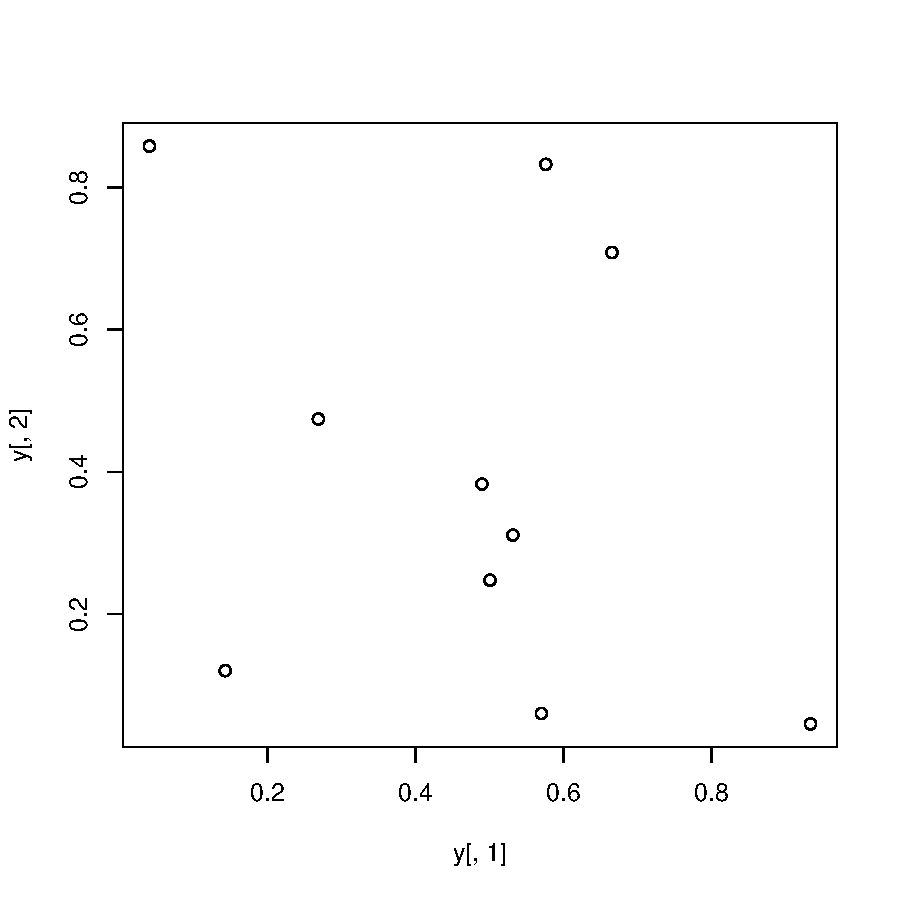
\includegraphics{fig--002}
%\caption{Here goes the caption.}
\label{fig:base_scatter}
\end{figure}
\end{frame}
%%%%%%%%%%%%%%%%%%%%%%%%%%%%%%%%% SLIDE %%%%%%%%%%%%%%%%%%%%%%%%%%%%%%%%%
\begin{frame}[containsverbatim]  
	\frametitle{Scatter Plot: all pairs}
\scriptsize
%<<echo=FALSE>>=
%options(width=70)
%@
\begin{figure}
  \centering
\begin{Schunk}
\begin{Sinput}
> pairs(y) 
\end{Sinput}
\end{Schunk}
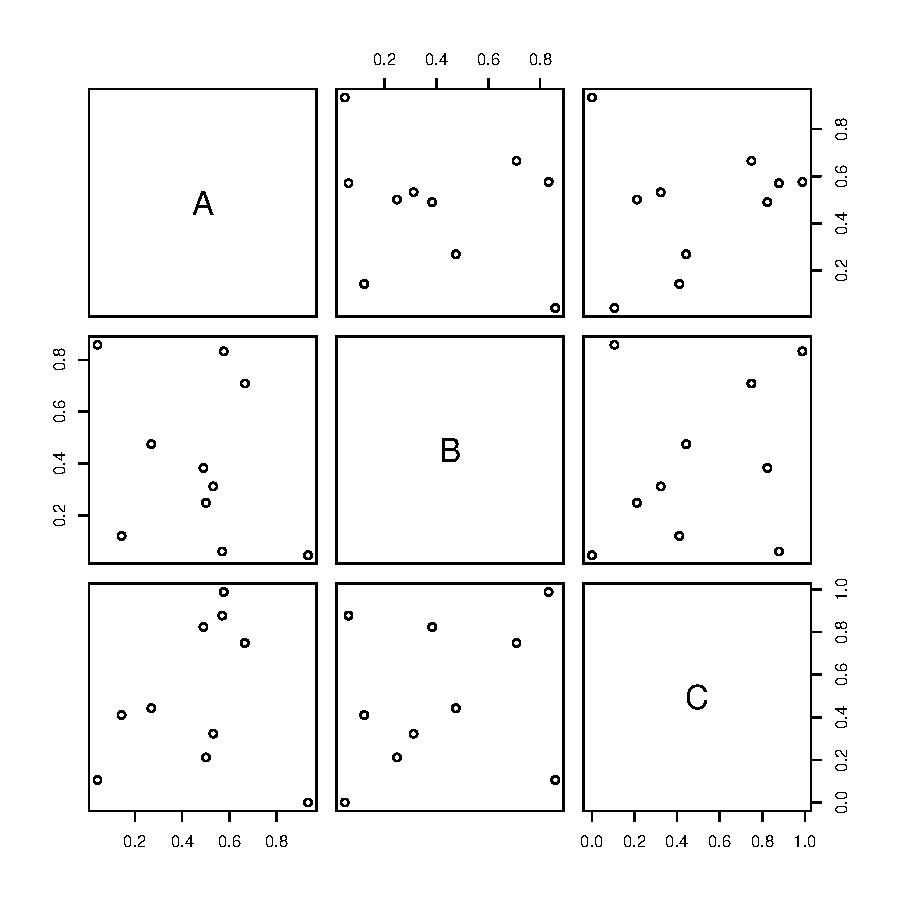
\includegraphics{fig--003}
%\caption{Here goes the caption.}
\label{fig:base_scatter_all}
\end{figure}
\end{frame}
%%%%%%%%%%%%%%%%%%%%%%%%%%%%%%%%% SLIDE %%%%%%%%%%%%%%%%%%%%%%%%%%%%%%%%%
\begin{frame}[containsverbatim]  
	\frametitle{Scatter Plot: with labels}
\scriptsize
\begin{figure}
  \centering
\begin{Schunk}
\begin{Sinput}
> plot(y[,1], y[,2], pch=20, col="red", main="Symbols and Labels")
> text(y[,1]+0.03, y[,2], rownames(y))
\end{Sinput}
\end{Schunk}
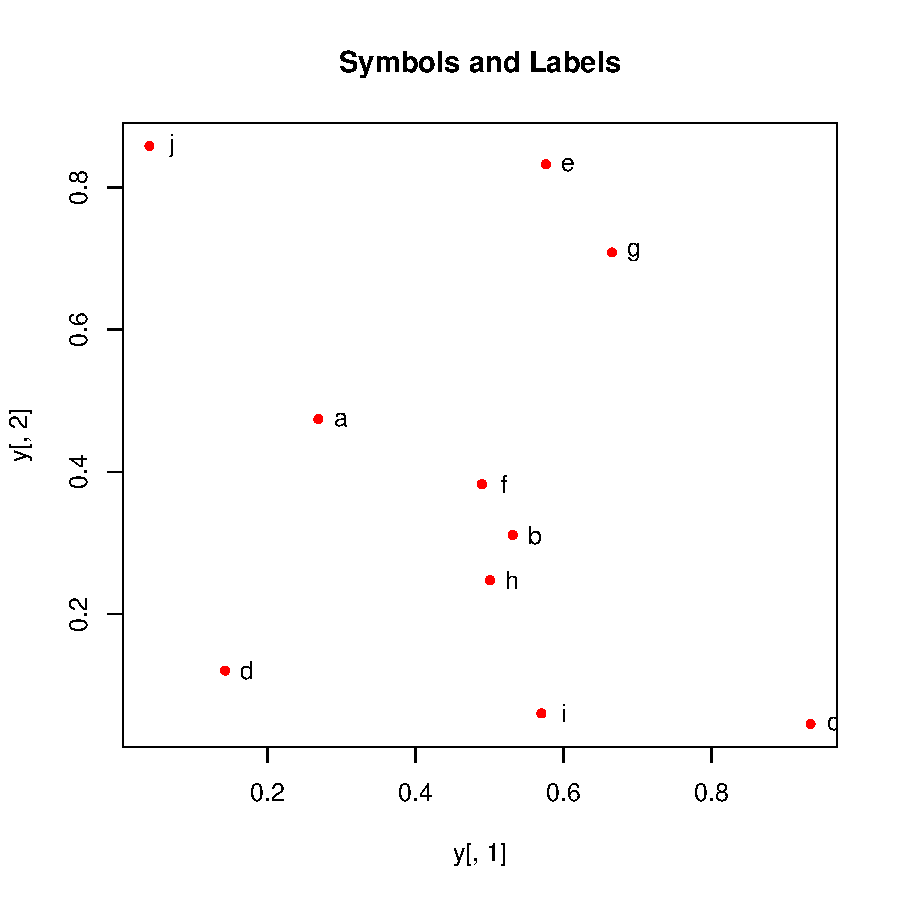
\includegraphics{fig--004}
%\caption{Here goes the caption.}
\label{fig:base_scatter_lab}
\end{figure}
\end{frame}
%%%%%%%%%%%%%%%%%%%%%%%%%%%%%%%%% SLIDE %%%%%%%%%%%%%%%%%%%%%%%%%%%%%%%%%
\begin{frame}[containsverbatim]  
	\frametitle{Scatter Plots: more examples}
\scriptsize
\textcolor{blue}{Print instead of symbols the row names}
\begin{Schunk}
\begin{Sinput}
> plot(y[,1], y[,2], type="n", main="Plot of Labels")
> text(y[,1], y[,2], rownames(y)) 
\end{Sinput}
\end{Schunk}
\textcolor{blue}{Usage of important plotting parameters}
\begin{Schunk}
\begin{Sinput}
> grid(5, 5, lwd = 2) 
> op <- par(mar=c(8,8,8,8), bg="lightblue")
> plot(y[,1], y[,2], type="p", col="red", cex.lab=1.2, cex.axis=1.2, 
+      cex.main=1.2, cex.sub=1, lwd=4, pch=20, xlab="x label", 
+      ylab="y label", main="My Main", sub="My Sub")
> par(op)
\end{Sinput}
\end{Schunk}
\begin{itemize}
\scriptsize
        \item[] \hspace{-0.8cm}\textcolor{blue}{Important arguments}
        \item \Rfunarg{mar}: specifies the margin sizes around the plotting area in order: \Rfunction{c(bottom, left, top, right)} 
        \item \Rfunarg{col}: color of symbols
        \item \Rfunarg{pch}: type of symbols, samples: \Rfunction{example(points)}
        \item \Rfunarg{lwd}: size of symbols
        \item \Rfunarg{cex.*}: control font sizes
        \item For details see \Rfunction{?par}
\end{itemize}
\end{frame}
%%%%%%%%%%%%%%%%%%%%%%%%%%%%%%%%% SLIDE %%%%%%%%%%%%%%%%%%%%%%%%%%%%%%%%%
\begin{frame}[containsverbatim]  
	\frametitle{Scatter Plots: more examples}
\scriptsize
\textcolor{blue}{Add a regression line to a plot}
\begin{Schunk}
\begin{Sinput}
> plot(y[,1], y[,2])
> myline <- lm(y[,2]~y[,1]); abline(myline, lwd=2) 
> summary(myline) 
\end{Sinput}
\end{Schunk}
\textcolor{blue}{Same plot as above, but on log scale}
\begin{Schunk}
\begin{Sinput}
> plot(y[,1], y[,2], log="xy") 
\end{Sinput}
\end{Schunk}
\textcolor{blue}{Add a mathematical expression to a plot}
\begin{Schunk}
\begin{Sinput}
> plot(y[,1], y[,2]); text(y[1,1], y[1,2], 
\end{Sinput}
\end{Schunk}
\end{frame}
%%%%%%%%%%%%%%%%%%%%%%%%%%%%%%%%% SLIDE %%%%%%%%%%%%%%%%%%%%%%%%%%%%%%%%%
\begin{frame}[containsverbatim]  
	\frametitle{Exercise 1: Scatter Plots}
\scriptsize
\begin{itemize}
        \item[Task 1] Generate scatter plot for first two columns in \Rfunction{iris} data frame and color dots by its \Rfunction{Species} column.
        \item[Task 2] Use the \Rfunarg{xlim/ylim} arguments to set limits on the x- and y-axes so that all data points are restricted to the left bottom quadrant of the plot. 
        \item[]\hspace{-1.1cm} Structure of iris data set:
\end{itemize}
\begin{Schunk}
\begin{Sinput}
> class(iris)
\end{Sinput}
\begin{Soutput}
[1] "data.frame"
\end{Soutput}
\begin{Sinput}
> iris[1:4,]
\end{Sinput}
\begin{Soutput}
  Sepal.Length Sepal.Width Petal.Length Petal.Width Species
1          5.1         3.5          1.4         0.2  setosa
2          4.9         3.0          1.4         0.2  setosa
3          4.7         3.2          1.3         0.2  setosa
4          4.6         3.1          1.5         0.2  setosa
\end{Soutput}
\begin{Sinput}
> table(iris$Species)
\end{Sinput}
\begin{Soutput}
    setosa versicolor  virginica 
        50         50         50 
\end{Soutput}
\end{Schunk}
\end{frame}
%%%%%%%%%%%%%%%%%%%%%%%%%%%%%%%%% SLIDE %%%%%%%%%%%%%%%%%%%%%%%%%%%%%%%%%
\begin{frame}[containsverbatim]  
	\frametitle{Line Plot: Single Data Set}
\scriptsize
%Plots a simple line graph.
\begin{figure}
  \centering
\begin{Schunk}
\begin{Sinput}
> plot(y[,1], type="l", lwd=2, col="blue") 
\end{Sinput}
\end{Schunk}
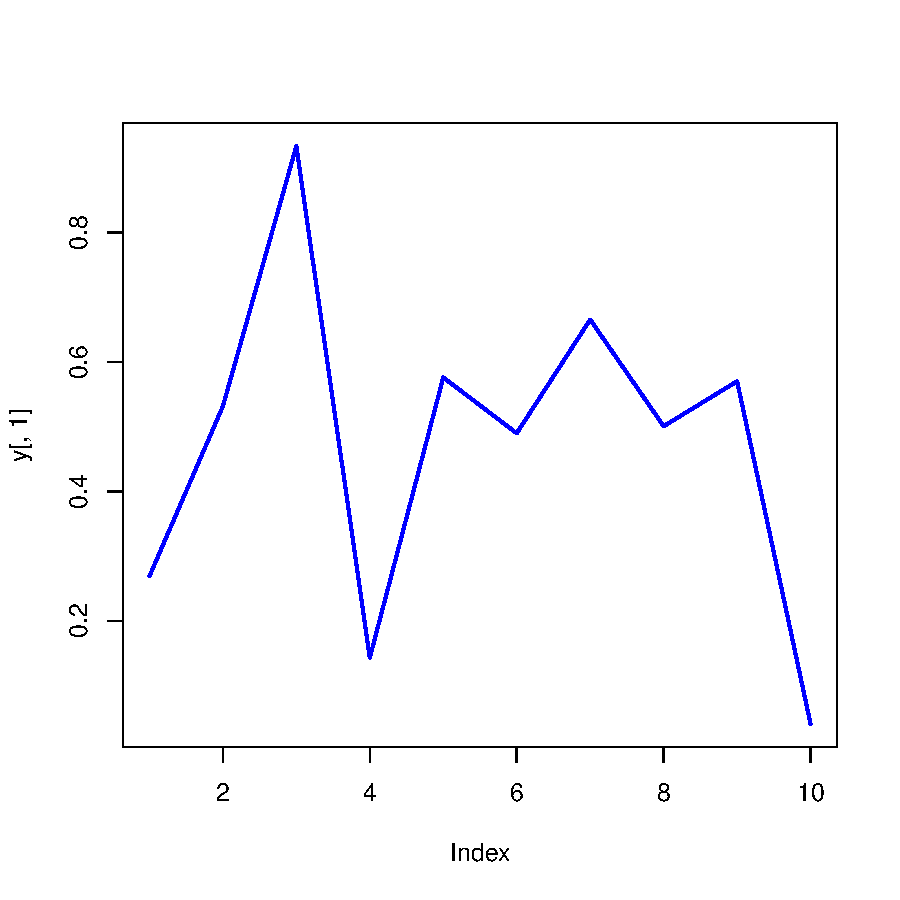
\includegraphics{fig--012}
%\caption{Here goes the caption.}
\label{fig:line_plot}
\end{figure}
\end{frame}
%%%%%%%%%%%%%%%%%%%%%%%%%%%%%%%%% SLIDE %%%%%%%%%%%%%%%%%%%%%%%%%%%%%%%%%
\begin{frame}[containsverbatim]  
	\frametitle{Line Plots: Many Data Sets}
\scriptsize
%Plots line graph for all columns in data frame \Rfunction{y}. The \Rfunction{split.screen} function is used in this example in a for loop to overlay several line graphs in the same plot. 
\tiny
\begin{figure}
  \centering
\begin{Schunk}
\begin{Sinput}
> split.screen(c(1,1)); 
\end{Sinput}
\begin{Soutput}
[1] 1
\end{Soutput}
\begin{Sinput}
> plot(y[,1], ylim=c(0,1), xlab="Measurement", ylab="Intensity", type="l", lwd=2, col=1)
> for(i in 2:length(y[1,])) { 
+ 	screen(1, new=FALSE)
+ 	plot(y[,i], ylim=c(0,1), type="l", lwd=2, col=i, xaxt="n", yaxt="n", ylab="", 
+              xlab="", main="", bty="n") 
+ }
> close.screen(all=TRUE) 
\end{Sinput}
\end{Schunk}
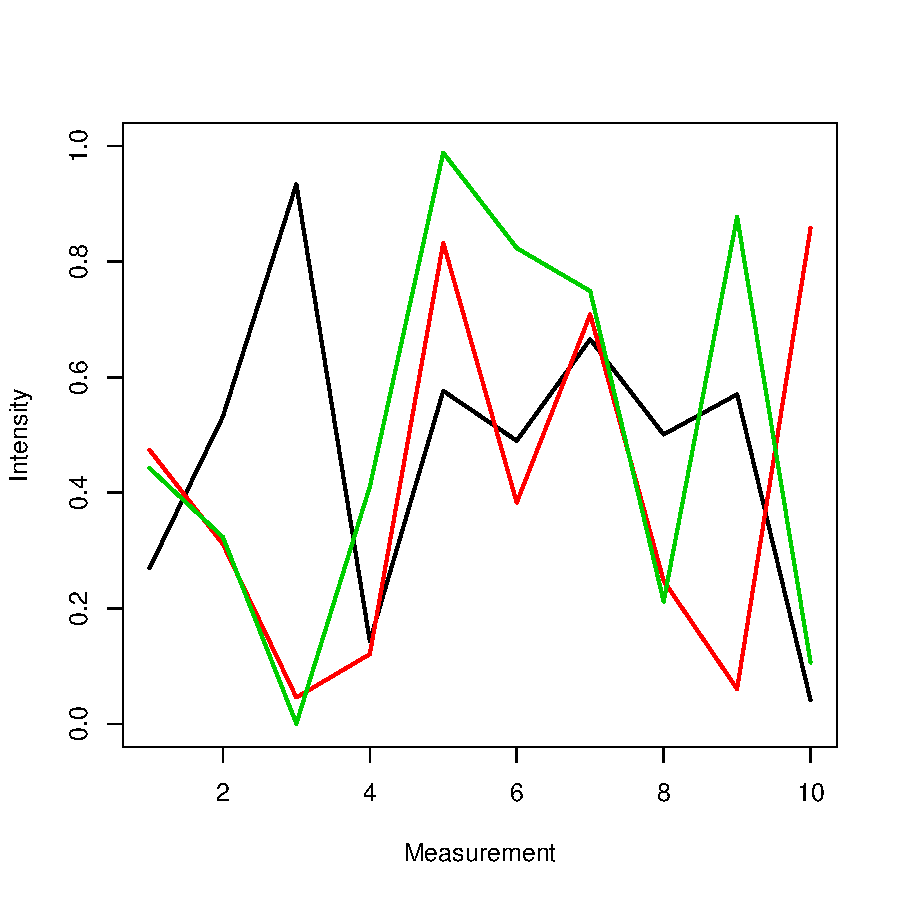
\includegraphics{fig--013}
%\caption{Here goes the caption.}
\label{fig:line_plot_many}
\end{figure}
\end{frame}
%%%%%%%%%%%%%%%%%%%%%%%%%%%%%%%%% SLIDE %%%%%%%%%%%%%%%%%%%%%%%%%%%%%%%%%
\begin{frame}[containsverbatim]  
	\frametitle{Bar Plot Basics}
\scriptsize
\begin{figure}
  \centering
\begin{Schunk}
\begin{Sinput}
> barplot(y[1:4,], ylim=c(0, max(y[1:4,])+0.3), beside=TRUE, 
+         legend=letters[1:4]) 
> text(labels=round(as.vector(as.matrix(y[1:4,])),2), x=seq(1.5, 13, by=1)
+      +sort(rep(c(0,1,2), 4)), y=as.vector(as.matrix(y[1:4,]))+0.04) 
\end{Sinput}
\end{Schunk}
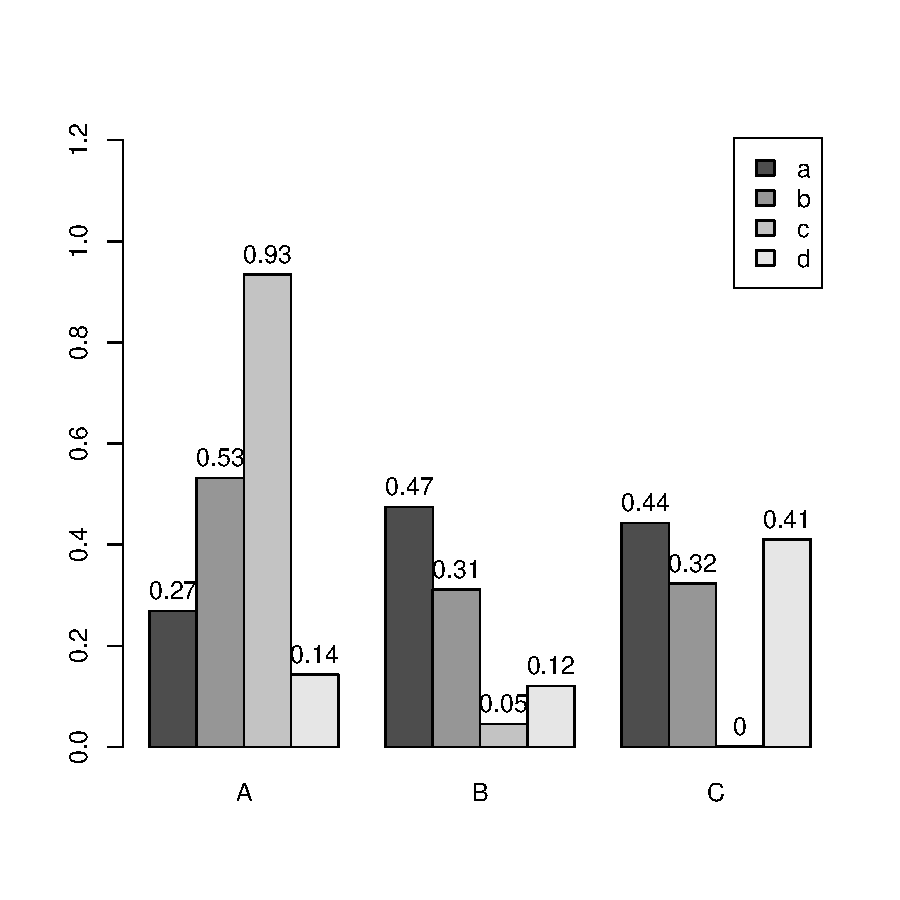
\includegraphics{fig--014}
%\caption{Here goes the caption.}
\label{fig:bar_plot1}
\end{figure}
\end{frame}
%%%%%%%%%%%%%%%%%%%%%%%%%%%%%%%%% SLIDE %%%%%%%%%%%%%%%%%%%%%%%%%%%%%%%%%
\begin{frame}[containsverbatim]  
	\frametitle{Bar Plots with Error Bars}
\scriptsize
\begin{figure}
  \centering
\begin{Schunk}
\begin{Sinput}
> bar <- barplot(m <- rowMeans(y) * 10, ylim=c(0, 10))
> stdev <- sd(t(y))
> arrows(bar, m, bar, m + stdev, length=0.15, angle = 90)
\end{Sinput}
\end{Schunk}
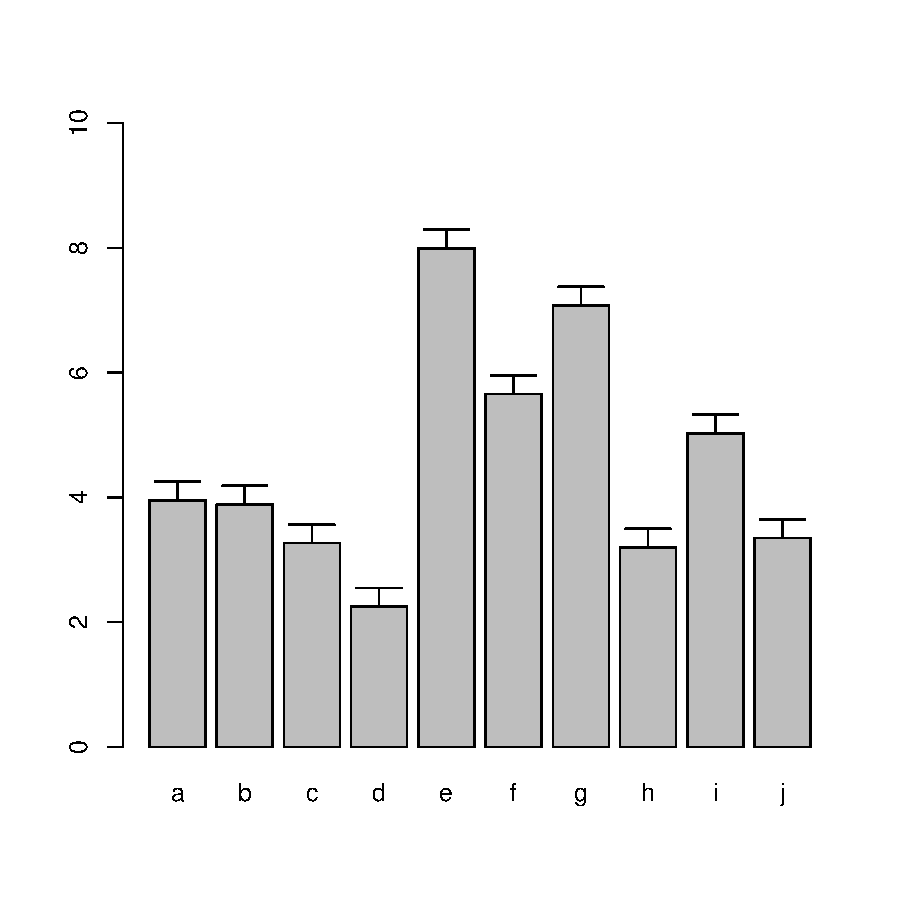
\includegraphics{fig--015}
%\caption{Here goes the caption.}
\label{ig:bar_plot2}
\end{figure}
\end{frame}
%%%%%%%%%%%%%%%%%%%%%%%%%%%%%%%%% SLIDE %%%%%%%%%%%%%%%%%%%%%%%%%%%%%%%%%
\begin{frame}[containsverbatim]  
	\frametitle{Histograms}
\scriptsize
\begin{figure}
  \centering
\begin{Schunk}
\begin{Sinput}
> hist(y, freq=TRUE, breaks=10)
\end{Sinput}
\end{Schunk}
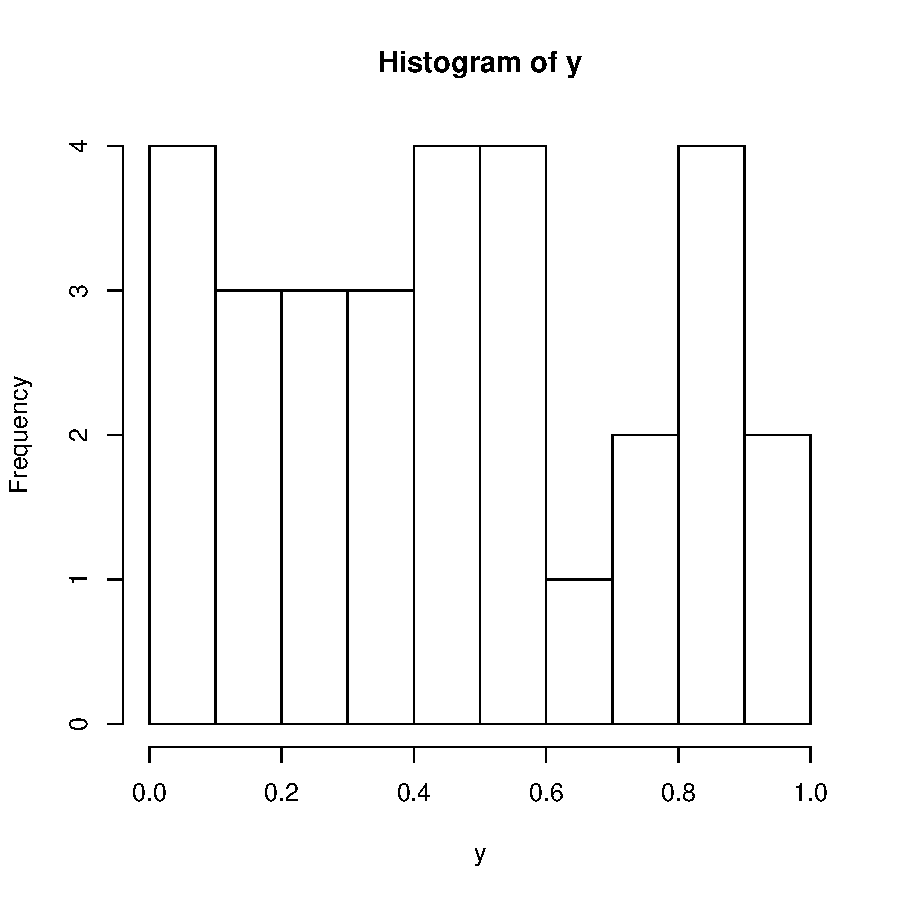
\includegraphics{fig--017}
%\caption{Here goes the caption.}
\label{fig:hist}
\end{figure}
\end{frame}
%%%%%%%%%%%%%%%%%%%%%%%%%%%%%%%%% SLIDE %%%%%%%%%%%%%%%%%%%%%%%%%%%%%%%%%
\begin{frame}[containsverbatim]  
	\frametitle{Density Plots}
\scriptsize
\begin{figure}
  \centering
\begin{Schunk}
\begin{Sinput}
> plot(density(y), col="red")
\end{Sinput}
\end{Schunk}
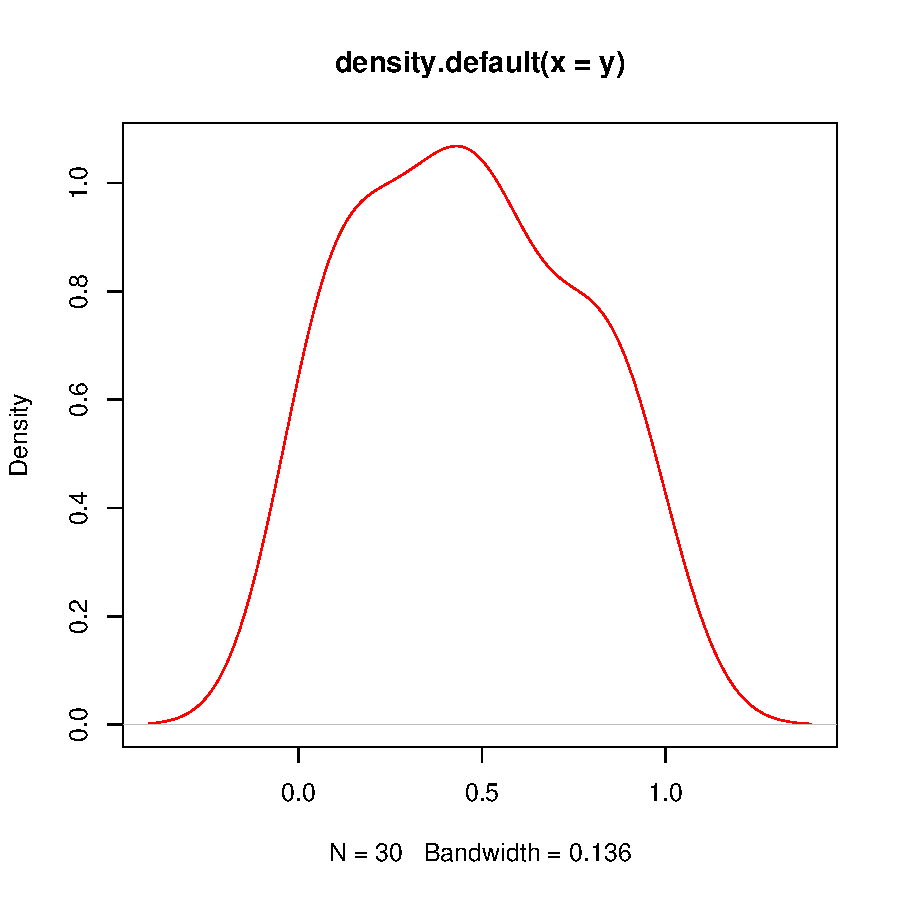
\includegraphics{fig--018}
%\caption{Here goes the caption.}
\label{fig:dens}
\end{figure}
\end{frame}
%%%%%%%%%%%%%%%%%%%%%%%%%%%%%%%%% SLIDE %%%%%%%%%%%%%%%%%%%%%%%%%%%%%%%%%
\begin{frame}[containsverbatim]  
	\frametitle{Pie Charts}
\scriptsize
\begin{figure}
  \centering
\begin{Schunk}
\begin{Sinput}
> pie(y[,1], col=rainbow(length(y[,1]), start=0.1, end=0.8), clockwise=TRUE)
> legend("topright", legend=row.names(y), cex=1.3, bty="n", pch=15, pt.cex=1.8, 
+ col=rainbow(length(y[,1]), start=0.1, end=0.8), ncol=1) 
\end{Sinput}
\end{Schunk}
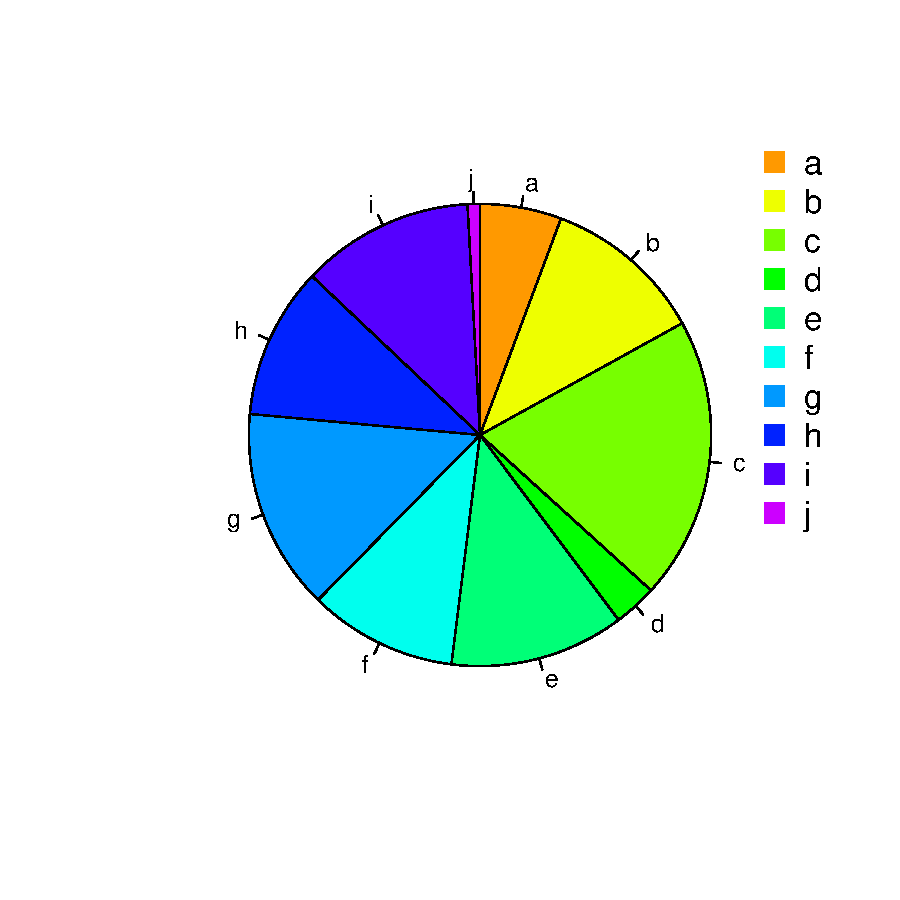
\includegraphics{fig--019}
%\caption{Here goes the caption.}
\label{fig:pie}
\end{figure}
\end{frame}
%%%%%%%%%%%%%%%%%%%%%%%%%%%%%%%%% SLIDE %%%%%%%%%%%%%%%%%%%%%%%%%%%%%%%%%
\begin{frame}[containsverbatim]  
	\frametitle{Color Selection Utilities}
\scriptsize
\textcolor{blue}{Default color palette and how to change it}
\begin{Schunk}
\begin{Sinput}
> palette()
\end{Sinput}
\begin{Soutput}
[1] "black"   "red"     "green3"  "blue"    "cyan"    "magenta" "yellow"  "gray"   
\end{Soutput}
\begin{Sinput}
> palette(rainbow(5, start=0.1, end=0.2))
> palette()
\end{Sinput}
\begin{Soutput}
[1] "#FF9900" "#FFBF00" "#FFE600" "#F2FF00" "#CCFF00"
\end{Soutput}
\begin{Sinput}
> palette("default")
\end{Sinput}
\end{Schunk}
\textcolor{blue}{The \Rfunction{gray} function allows to select any type of gray shades by providing values from 0 to 1}
\begin{Schunk}
\begin{Sinput}
> gray(seq(0.1, 1, by= 0.2))
\end{Sinput}
\begin{Soutput}
[1] "#1A1A1A" "#4D4D4D" "#808080" "#B3B3B3" "#E6E6E6"
\end{Soutput}
\end{Schunk}
\textcolor{blue}{Color gradients with \Rfunction{colorpanel} function from \Rpackage{gplots} library}
\begin{Schunk}
\begin{Sinput}
> library(gplots)
> colorpanel(5, "darkblue", "yellow", "white")
\end{Sinput}
\end{Schunk}
Much more on colors in R see Earl Glynn's color chart \href{http://research.stowers-institute.org/efg/R/Color/Chart/}{{\beamerbutton{Link}}} 
\end{frame}
%%%%%%%%%%%%%%%%%%%%%%%%%%%%%%%%% SLIDE %%%%%%%%%%%%%%%%%%%%%%%%%%%%%%%%%
\begin{frame}[containsverbatim]  
	\frametitle{Arranging Several Plots on Single Page}
\scriptsize
\textcolor{blue}{With \Rfunction{par(mfrow=c(nrow,ncol))} one can define how several plots are arranged next to each other.}
\begin{figure}
  \centering
\begin{Schunk}
\begin{Sinput}
> par(mfrow=c(2,3)); for(i in 1:6) { plot(1:10) } 
\end{Sinput}
\end{Schunk}
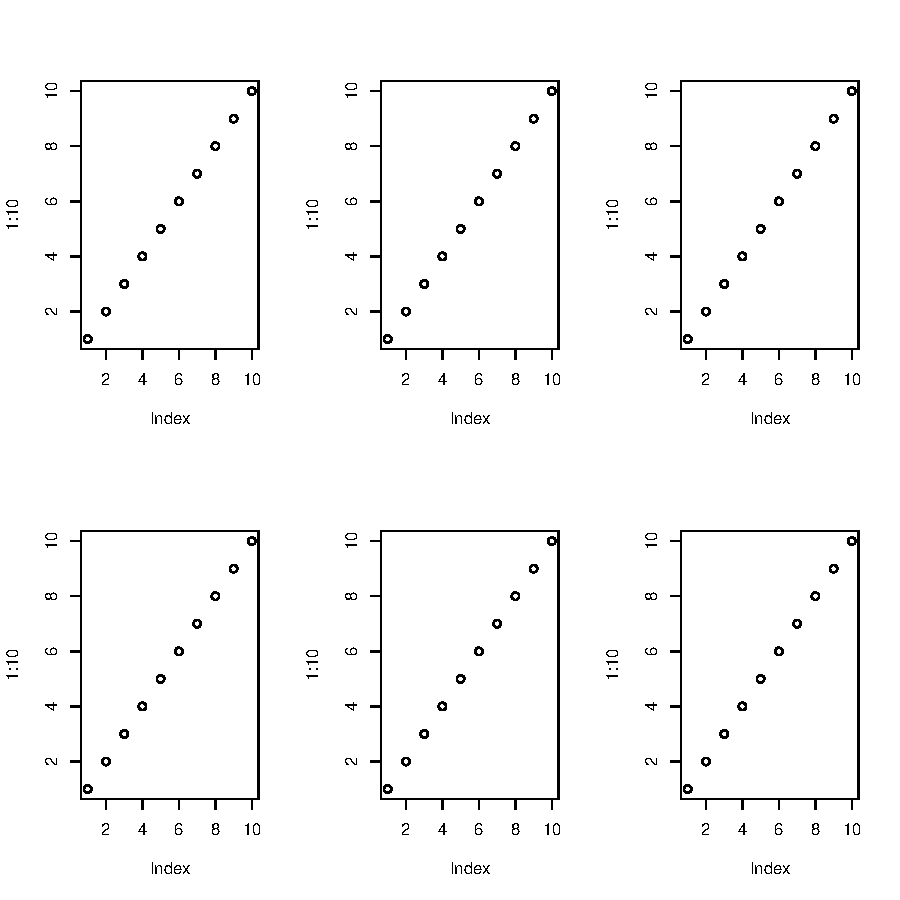
\includegraphics{fig--023}
%\caption{Here goes the caption.}
\label{fig:arrange1}
\end{figure}
\end{frame}
%%%%%%%%%%%%%%%%%%%%%%%%%%%%%%%%% SLIDE %%%%%%%%%%%%%%%%%%%%%%%%%%%%%%%%%
\begin{frame}[containsverbatim]  
	\frametitle{Arranging Plots with Variable Width}
\scriptsize
\textcolor{blue}{The \Rfunction{layout} function allows to divide the plotting device into variable numbers of rows and columns with the column-widths and the row-heights specified in the respective arguments.}
\begin{figure}
  \centering
\begin{Schunk}
\begin{Sinput}
> nf <- layout(matrix(c(1,2,3,3), 2, 2, byrow=TRUE), c(3,7), c(5,5), 
+              respect=TRUE)
> # layout.show(nf)
> for(i in 1:3) { barplot(1:10) } 
\end{Sinput}
\end{Schunk}
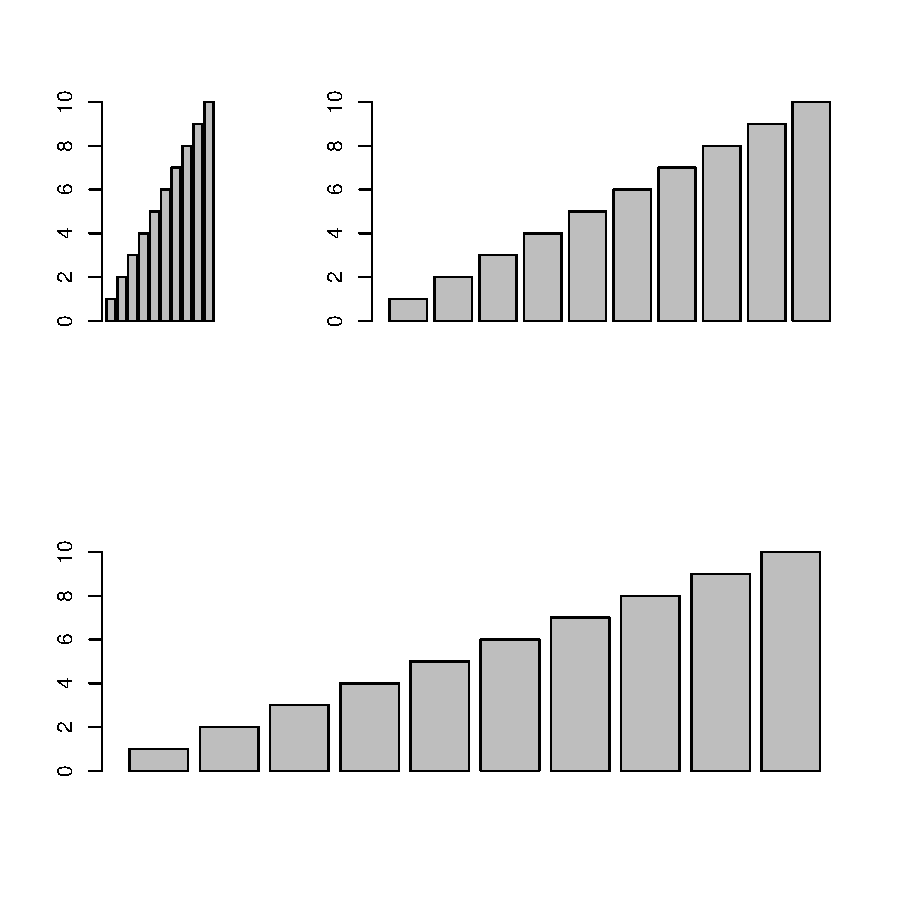
\includegraphics{fig--024}
%\caption{Here goes the caption.}
\label{fig:arrange2}
\end{figure}
\end{frame}
%%%%%%%%%%%%%%%%%%%%%%%%%%%%%%%%% SLIDE %%%%%%%%%%%%%%%%%%%%%%%%%%%%%%%%%
\begin{frame}[containsverbatim]  
	\frametitle{Saving Graphics to Files}
\scriptsize
\textcolor{blue}{After the \Rfunction{pdf()} command all graphs are redirected to file \Rfunction{test.pdf}. Works for all common formats similarly: jpeg, png, ps, tiff, ...}
\begin{Schunk}
\begin{Sinput}
> pdf("test.pdf"); plot(1:10, 1:10); dev.off() 
\end{Sinput}
\end{Schunk}
\textcolor{blue}{Generates Scalable Vector Graphics (SVG) files that can be edited in vector graphics programs, such as InkScape.}
\begin{Schunk}
\begin{Sinput}
> svg("test.svg"); plot(1:10, 1:10); dev.off() 
\end{Sinput}
\end{Schunk}
\end{frame}
%%%%%%%%%%%%%%%%%%%%%%%%%%%%%%%%% SLIDE %%%%%%%%%%%%%%%%%%%%%%%%%%%%%%%%%
\begin{frame}[containsverbatim]  
	\frametitle{Exercise 2: Bar Plots}
\scriptsize
\begin{itemize}
        \item[Task 1] Calculate the mean values for the \Rfunction{Species} components of the first four columns in the \Rfunction{iris} data set. Organize the results in a matrix where the row names are the unique values from the \Rfunction{iris Species} column and the column names are the same as in the first four \Rfunction{iris} columns. 
        \item[Task 2] Generate two bar plots: one with stacked bars and one with horizontally arranged bars. 
        \item[]\hspace{-1.1cm} Structure of iris data set:
\end{itemize}
\begin{Schunk}
\begin{Sinput}
> class(iris)
\end{Sinput}
\begin{Soutput}
[1] "data.frame"
\end{Soutput}
\begin{Sinput}
> iris[1:4,]
\end{Sinput}
\begin{Soutput}
  Sepal.Length Sepal.Width Petal.Length Petal.Width Species
1          5.1         3.5          1.4         0.2  setosa
2          4.9         3.0          1.4         0.2  setosa
3          4.7         3.2          1.3         0.2  setosa
4          4.6         3.1          1.5         0.2  setosa
\end{Soutput}
\begin{Sinput}
> table(iris$Species)
\end{Sinput}
\begin{Soutput}
    setosa versicolor  virginica 
        50         50         50 
\end{Soutput}
\end{Schunk}
\end{frame}
%%%%%%%%%%%%%%%%%%%%%%%%%%%%%%%%% slide %%%%%%%%%%%%%%%%%%%%%%%%%%%%%%%%%
\subsection{Grid Graphics}
%%%%%%%%%%%%%%%%%%%%%%%%%%%%%%%%% SLIDE %%%%%%%%%%%%%%%%%%%%%%%%%%%%%%%%%
\begin{frame}[containsverbatim]  
	\frametitle{grid Graphics Environment}
\begin{itemize}
	\item What is \Rpackage{grid}?
        \begin{itemize}
		\item Low-level graphics system 
		\item Highly flexible and controllable system
		\item Does not provide high-level functions 
		\item Intended as development environment for custom plotting functions 
		\item Pre-installed on new R distributions
        \end{itemize}
        \item Documentation and Help
        \begin{itemize}
                \item Manual \href{http://www.stat.auckland.ac.nz/~paul/grid/grid.html}{{\beamerbutton{Link}}}
                \item Book \href{http://www.stat.auckland.ac.nz/~paul/RGraphics/rgraphics.html}{{\beamerbutton{Link}}}
        \end{itemize}
\end{itemize}
\end{frame}
%%%%%%%%%%%%%%%%%%%%%%%%%%%%%%%%% slide %%%%%%%%%%%%%%%%%%%%%%%%%%%%%%%%%
\subsection{lattice}
%%%%%%%%%%%%%%%%%%%%%%%%%%%%%%%%% SLIDE %%%%%%%%%%%%%%%%%%%%%%%%%%%%%%%%%
\begin{frame}[containsverbatim]  
	\frametitle{lattice Environment}
\begin{itemize}
	\item What is \Rpackage{lattice}?
        \begin{itemize}
		\item High-level graphics system 
		\item Developed by Deepayan Sarkar 
		\item Implements Trellis graphics system from S-Plus
		\item Simplifies high-level plotting tasks: arranging complex graphical features 
		\item Syntax similar to R's base graphics
        \end{itemize}
        \item Documentation and Help
        \begin{itemize}
                \item Manual \href{http://lmdvr.r-forge.r-project.org}{{\beamerbutton{Link}}}
                \item Intro \href{http://www.his.sunderland.ac.uk/~cs0her/Statistics/UsingLatticeGraphicsInR.htm}{{\beamerbutton{Link}}}
                \item Book \href{http://www.amazon.com/Lattice-Multivariate-Data-Visualization-Use/dp/0387759689}{{\beamerbutton{Link}}} 
		\item \Rfunction{library(help=lattice)} opens a list of all functions available in the lattice package
		\item Accessing and changing global parameters: \Rfunction{?lattice.options} and \Rfunction{?trellis.device}
        \end{itemize}
\end{itemize}
\end{frame}
%%%%%%%%%%%%%%%%%%%%%%%%%%%%%%%%% SLIDE %%%%%%%%%%%%%%%%%%%%%%%%%%%%%%%%%
\begin{frame}[containsverbatim]  
	\frametitle{Scatter Plot Sample}
\scriptsize
\begin{figure}
  \centering
\begin{Schunk}
\begin{Sinput}
> library(lattice)
> p1 <- xyplot(1:8 ~ 1:8 | rep(LETTERS[1:4], each=2), as.table=TRUE) 
> plot(p1)
\end{Sinput}
\end{Schunk}
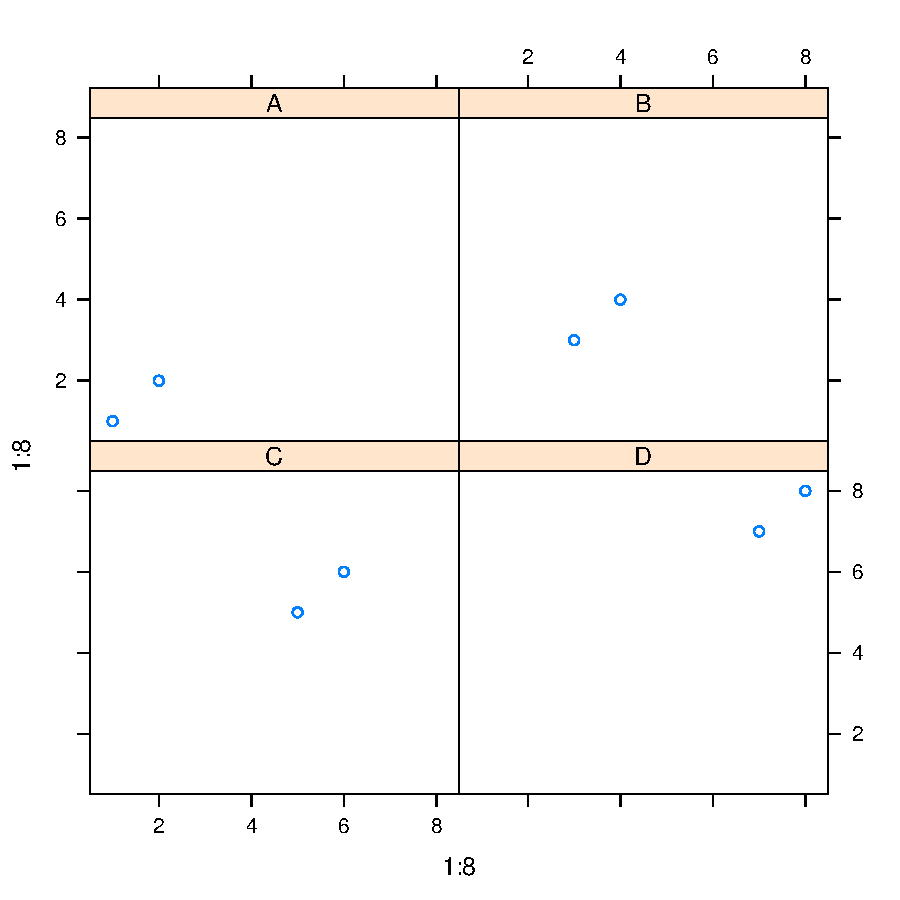
\includegraphics{fig--029}
%\caption{Here goes the caption.}
\label{fig:p1}
\end{figure}
\end{frame}
%%%%%%%%%%%%%%%%%%%%%%%%%%%%%%%%% SLIDE %%%%%%%%%%%%%%%%%%%%%%%%%%%%%%%%%
\begin{frame}[containsverbatim]  
	\frametitle{Line Plot Sample}
\scriptsize
\begin{figure}
  \centering
\begin{Schunk}
\begin{Sinput}
> library(lattice)
> p2 <- parallelplot(~iris[1:4] | Species, iris, horizontal.axis = FALSE, 
+               layout = c(1, 3, 1))  
> plot(p2)
\end{Sinput}
\end{Schunk}
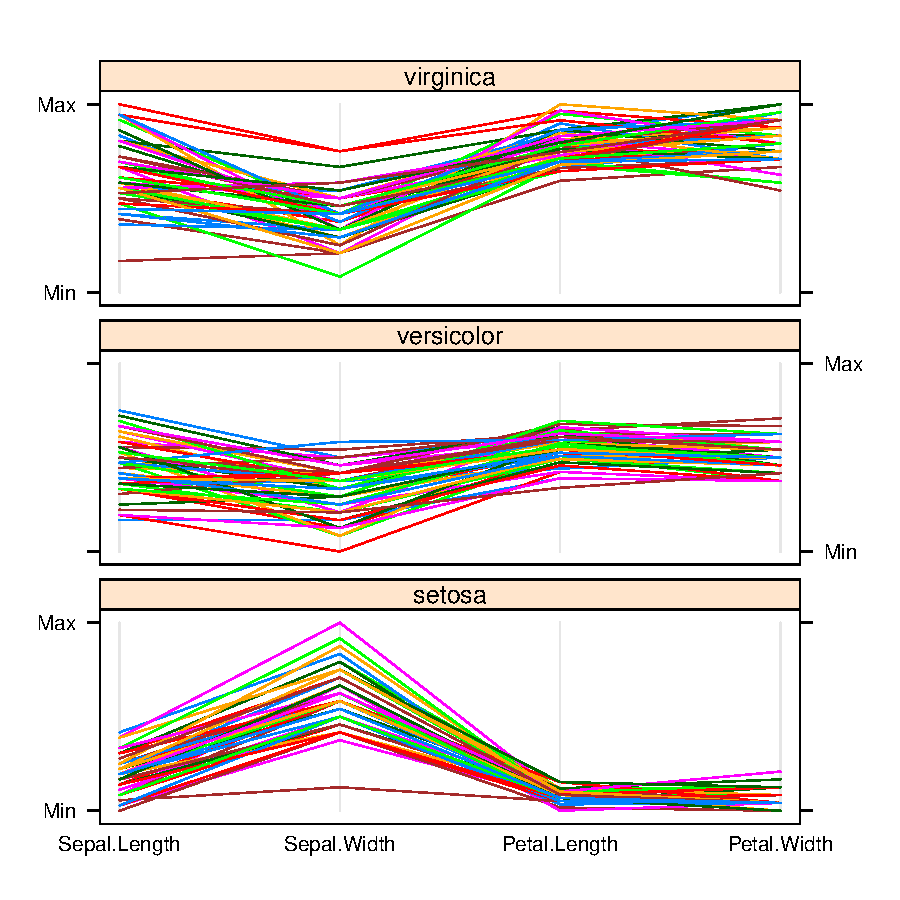
\includegraphics{fig--030}
%\caption{Here goes the caption.}
\label{fig:p2}
\end{figure}
\end{frame}
%%%%%%%%%%%%%%%%%%%%%%%%%%%%%%%%% slide %%%%%%%%%%%%%%%%%%%%%%%%%%%%%%%%%
\subsection{ggplot2}
%%%%%%%%%%%%%%%%%%%%%%%%%%%%%%%%% SLIDE %%%%%%%%%%%%%%%%%%%%%%%%%%%%%%%%%
\begin{frame}[containsverbatim]  
	\frametitle{ggplot2 Environment}
\begin{itemize}
	\item What is \Rpackage{ggplot2}?
        \begin{itemize}
		\item High-level graphics system
		\item Implements grammar of graphics from Leland Wilkinson \href{http://www.amazon.com/Grammar-Graphics-Leland-Wilkinson/dp/0387987746}{{\beamerbutton{Link}}} 
		\item Streamlines many graphics workflows for complex plots
		\item Syntax centered around main \Rfunction{ggplot} function 
		\item Simpler \Rfunction{qplot} function provides many shortcuts
        \end{itemize}
        \item Documentation and Help
        \begin{itemize}
                \item Manual \href{http://had.co.nz/ggplot2/}{{\beamerbutton{Link}}}
                \item Intro \href{http://www.ling.upenn.edu/~joseff/rstudy/summer2010_ggplot2_intro.html}{{\beamerbutton{Link}}}
                \item Book \href{http://had.co.nz/ggplot2/book/}{{\beamerbutton{Link}}} 
                \item Cookbook for R \href{http://www.cookbook-r.com/Graphs/}{{\beamerbutton{Link}}} 
        \end{itemize}
\end{itemize}
\end{frame}
%%%%%%%%%%%%%%%%%%%%%%%%%%%%%%%%% SLIDE %%%%%%%%%%%%%%%%%%%%%%%%%%%%%%%%%
\begin{frame}[containsverbatim]  
	\frametitle{ggplot2 Usage}
\begin{itemize}
	\item \Rfunction{ggplot} function accepts two arguments
        \begin{itemize}
		\item Data set to be plotted 
		\item Aesthetic mappings provided by \Rfunction{aes} function
        \end{itemize}
	\item Additional parameters such as geometric objects (e.g. points, lines, bars) are passed on by appending them with \Rfunction{+} as separator. 
	\item List of available \Rfunction{geom\_*} functions: \href{http://docs.ggplot2.org/current/}{{\beamerbutton{Link}}} 
	\item Settings of plotting theme can be accessed with the command \Rfunction{theme\_get()} and its settings can be changed with \Rfunction{theme()}. 
	\item Preferred input data object 
        \begin{itemize}
		\item \Rfunction{qplot}: \Robject{data.frame} (support for \Robject{vector, matrix, ...})
		\item \Rfunction{ggplot}: \Robject{data.frame}
        \end{itemize}
	\item Packages with convenience utilities to create expected inputs
        \begin{itemize}
		\item \Rpackage{plyr} 
		\item \Rpackage{reshape}
        \end{itemize}
\end{itemize}
\end{frame}
%%%%%%%%%%%%%%%%%%%%%%%%%%%%%%%%% SLIDE %%%%%%%%%%%%%%%%%%%%%%%%%%%%%%%%%
\begin{frame}[containsverbatim]  
	\frametitle{qplot Function}
\begin{itemize}
	\item \Rfunction{qplot} syntax is similar to R's basic \Rfunction{plot} function
	\item Arguments: 
        \begin{itemize}
        	\item \Rfunction{x}: x-coordinates (\textit{e.g.} \Rfunction{col1})
		\item \Rfunction{y}: y-coordinates (\textit{e.g.} \Rfunction{col2})
		\item \Rfunction{data}: data frame with corresponding column names
		\item \Rfunction{xlim, ylim}: \textit{e.g.} \Rfunction{xlim=c(0,10)} 
		\item \Rfunction{log}: \textit{e.g.} \Rfunction{log="x" or log="xy"}
		\item \Rfunction{main}: main title; see \Rfunction{?plotmath} for mathematical formula
		\item \Rfunction{xlab, ylab}: labels for the x- and y-axes
		\item \Rfunction{color, shape, size}
		\item \Rfunction{...}: many arguments accepted by \Rfunction{plot} function
	\end{itemize}
\end{itemize}
\end{frame}
%%%%%%%%%%%%%%%%%%%%%%%%%%%%%%%%% slide %%%%%%%%%%%%%%%%%%%%%%%%%%%%%%%%%
\begin{frame}[containsverbatim]  
	\frametitle{qplot: Scatter Plots}
\vspace{0cm}
\scriptsize 
\textcolor{blue}{Create sample data}
\begin{Schunk}
\begin{Sinput}
> library(ggplot2)
> x <- sample(1:10, 10); y <- sample(1:10, 10); cat <- rep(c("A", "B"), 5)
\end{Sinput}
\end{Schunk}
\textcolor{blue}{Simple scatter plot}
\begin{Schunk}
\begin{Sinput}
> qplot(x, y, geom="point")
\end{Sinput}
\end{Schunk}
\textcolor{blue}{Prints dots with different sizes and colors}
\begin{Schunk}
\begin{Sinput}
> qplot(x, y, geom="point", size=x, color=cat, 
+       main="Dot Size and Color Relative to Some Values")
\end{Sinput}
\end{Schunk}
\textcolor{blue}{Drops legend}
\begin{Schunk}
\begin{Sinput}
> qplot(x, y, geom="point", size=x, color=cat) + 
+       theme(legend.position = "none")
\end{Sinput}
\end{Schunk}
\textcolor{blue}{Plot different shapes}
\begin{Schunk}
\begin{Sinput}
> qplot(x, y, geom="point", size=5, shape=cat)
\end{Sinput}
\end{Schunk}
\end{frame}
%%%%%%%%%%%%%%%%%%%%%%%%%%%%%%%%% slide %%%%%%%%%%%%%%%%%%%%%%%%%%%%%%%%%
\begin{frame}[containsverbatim]  
	\frametitle{qplot: Scatter Plot with qplot}
\scriptsize 
\begin{figure}
  \centering
\begin{Schunk}
\begin{Sinput}
> p <- qplot(x, y, geom="point", size=x, color=cat, 
+             main="Dot Size and Color Relative to Some Values") + 
+      theme(legend.position = "none")
> print(p)
\end{Sinput}
\end{Schunk}
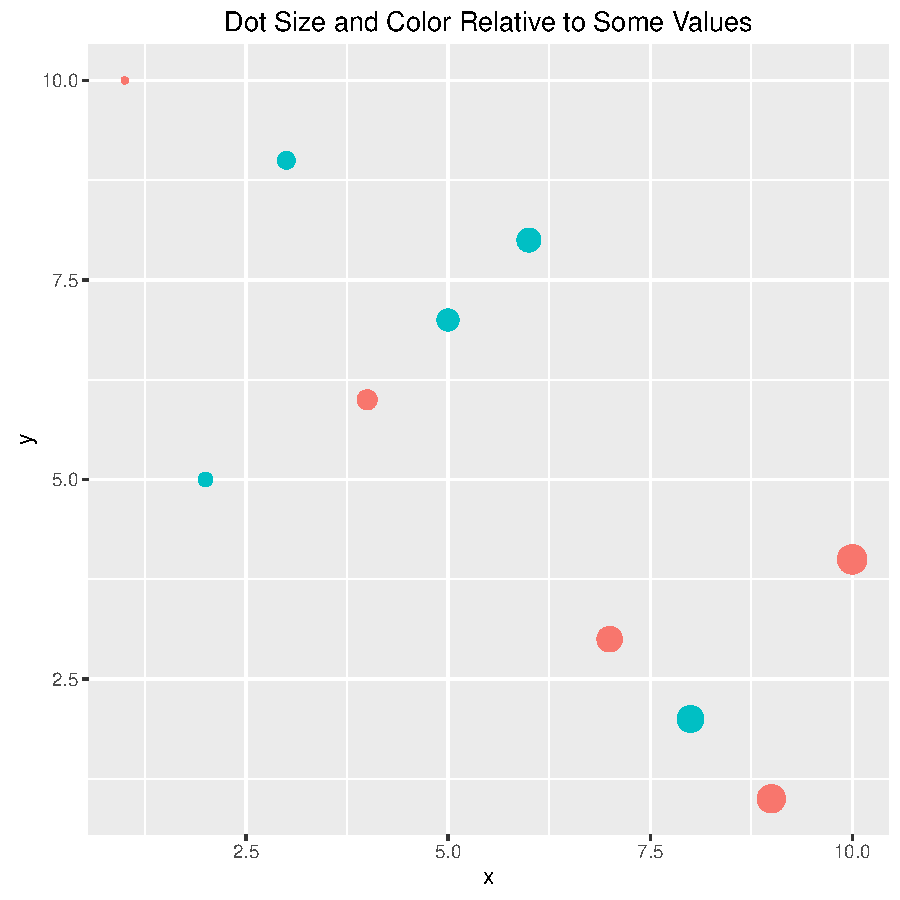
\includegraphics{fig--036}
\label{fig:qplotscatter}
\end{figure}
\end{frame}
%%%%%%%%%%%%%%%%%%%%%%%%%%%%%%%%% slide %%%%%%%%%%%%%%%%%%%%%%%%%%%%%%%%%
\begin{frame}[containsverbatim]  
	\frametitle{qplot: Scatter Plot with Regression Line}
\scriptsize 
\begin{figure}
  \centering
\begin{Schunk}
\begin{Sinput}
> set.seed(1410)
> dsmall <- diamonds[sample(nrow(diamonds), 1000), ]
> p <- qplot(carat, price, data = dsmall, geom = c("point", "smooth")) +
+            geom_smooth(method="lm")
> print(p)
\end{Sinput}
\end{Schunk}
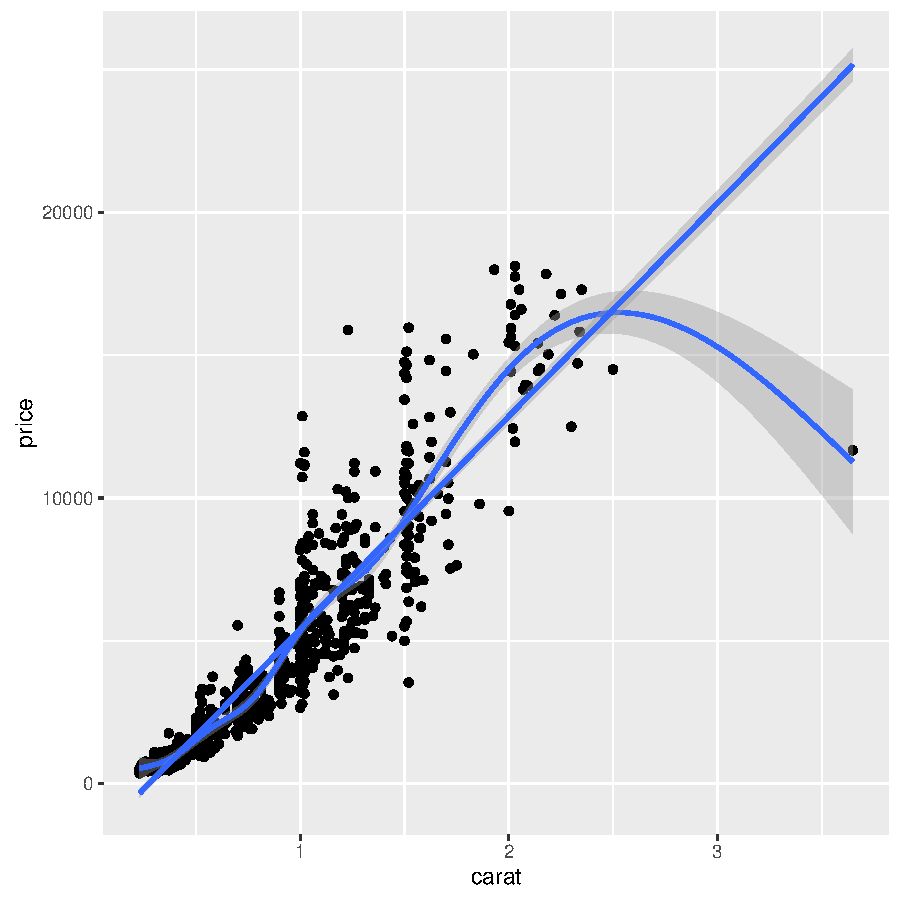
\includegraphics{fig--037}
\label{fig:qplotscatter}
\end{figure}
\end{frame}
%%%%%%%%%%%%%%%%%%%%%%%%%%%%%%%%% slide %%%%%%%%%%%%%%%%%%%%%%%%%%%%%%%%%
\begin{frame}[containsverbatim]  
	\frametitle{qplot: Scatter Plot with Local Regression Curve (loess)}
\scriptsize 
\begin{figure}
  \centering
\begin{Schunk}
\begin{Sinput}
> p <- qplot(carat, price, data=dsmall, geom=c("point", "smooth")) 
> print(p) # Setting se=FALSE removes error shade
\end{Sinput}
\end{Schunk}
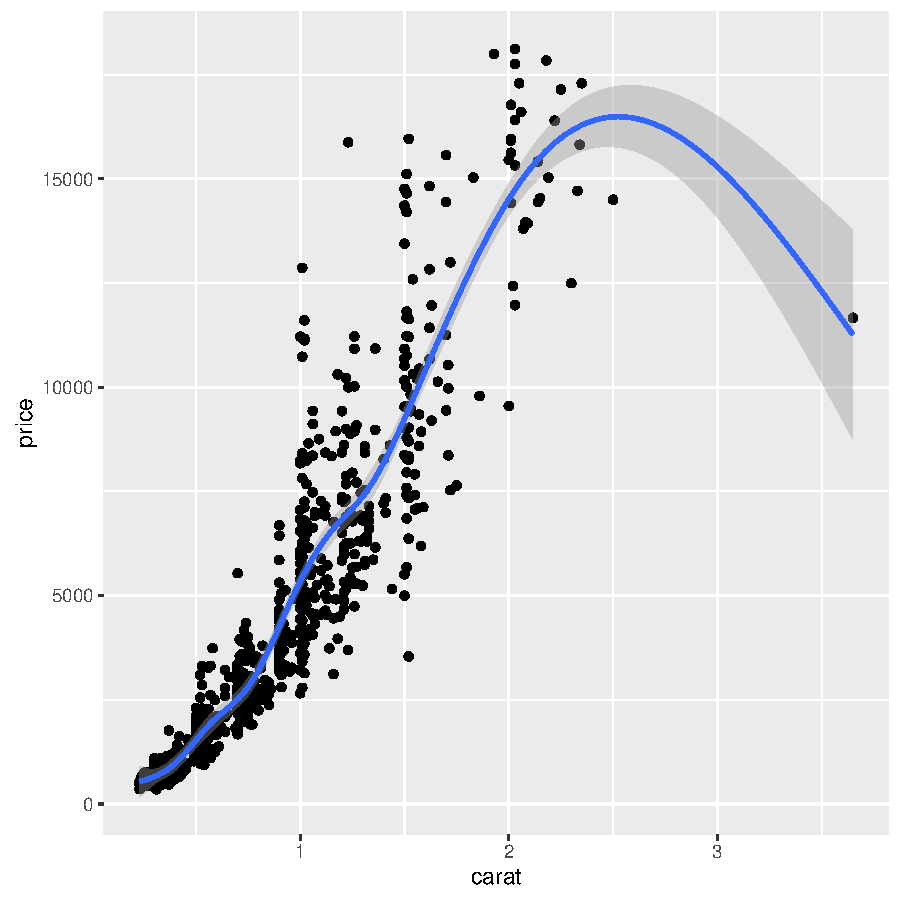
\includegraphics{fig--038}
\label{fig:qplotscatter}
\end{figure}
\end{frame}
%%%%%%%%%%%%%%%%%%%%%%%%%%%%%%%%% SLIDE %%%%%%%%%%%%%%%%%%%%%%%%%%%%%%%%%
\begin{frame}[containsverbatim]  
	\frametitle{ggplot Function}
\scriptsize
\begin{itemize}
	\item More important than \Rfunction{qplot} to access full functionality of \Rpackage {ggplot2} 
	\item Main arguments
        \begin{itemize}
	\scriptsize
        	\item data set, usually a \Rfunction{data.frame}
		\item aesthetic mappings provided by \Rfunction{aes} function
	\end{itemize}
	\item General \Rfunction{ggplot} syntax
        \begin{itemize}
	\scriptsize
        	\item \Rfunction{ggplot(data, aes(...)) + geom\_*() + ... + stat\_*() + ...}
	\end{itemize}
	\item Layer specifications
        \begin{itemize}
	\scriptsize
        	\item \Rfunction{geom\_*(mapping, data, ..., geom, position)}
		\item \Rfunction{stat\_*(mapping, data, ..., stat, position)}
	\end{itemize}
	\item Additional components
        \begin{itemize}
	\scriptsize
        	\item \Rfunction{scales}
		\item \Rfunction{coordinates} 
		\item \Rfunction{facet}
	\end{itemize}
	\item aes() mappings can be passed on to all components (\Rfunction{ggplot, geom\_*}, etc.). Effects are global when passed on to ggplot() and local for other components.
        \begin{itemize}
	\scriptsize
        	\item \Rfunction{x, y}
		\item \Rfunction{color}: grouping vector (factor) 
		\item \Rfunction{group}: grouping vector (factor)
	\end{itemize}
\end{itemize}
\end{frame}
%%%%%%%%%%%%%%%%%%%%%%%%%%%%%%%%% SLIDE %%%%%%%%%%%%%%%%%%%%%%%%%%%%%%%%%
\begin{frame}[containsverbatim]  
	\frametitle{Changing Plotting Themes with ggplot}
\scriptsize
\begin{itemize}
	\item Theme settings can be accessed with \Rfunction{theme\_get()}
	\item Their settings can be changed with \Rfunction{theme()} 
	\item Some examples
        \begin{itemize}
	\scriptsize
        	\item Change background color to white \\
		\tiny
		\Rfunction{... + theme(panel.background=element\_rect(fill = "white", colour = "black"))} 
	\end{itemize}
\end{itemize}
\end{frame}
%%%%%%%%%%%%%%%%%%%%%%%%%%%%%%%%% slide %%%%%%%%%%%%%%%%%%%%%%%%%%%%%%%%%
\begin{frame}[containsverbatim]  
	\frametitle{Storing ggplot Specifications}
\vspace{0cm}
\scriptsize 
\textcolor{blue}{Plots and layers can be stored in variables}
\begin{Schunk}
\begin{Sinput}
> p <- ggplot(dsmall, aes(carat, price)) + geom_point() 
> p # or print(p)
\end{Sinput}
\end{Schunk}
\textcolor{blue}{Returns information about data and aesthetic mappings followed by each layer}
\begin{Schunk}
\begin{Sinput}
> summary(p) 
\end{Sinput}
\end{Schunk}
\textcolor{blue}{Prints dots with different sizes and colors}
\begin{Schunk}
\begin{Sinput}
> bestfit <- geom_smooth(methodw = "lm", se = F, color = alpha("steelblue", 0.5), size = 2)
> p + bestfit # Plot with custom regression line
\end{Sinput}
\end{Schunk}
\textcolor{blue}{Syntax to pass on other data sets}
\begin{Schunk}
\begin{Sinput}
> p %+% diamonds[sample(nrow(diamonds), 100),] 
\end{Sinput}
\end{Schunk}
\textcolor{blue}{Saves plot stored in variable p to file}
\begin{Schunk}
\begin{Sinput}
> ggsave(p, file="myplot.pdf") 
\end{Sinput}
\end{Schunk}
\end{frame}
%%%%%%%%%%%%%%%%%%%%%%%%%%%%%%%%% slide %%%%%%%%%%%%%%%%%%%%%%%%%%%%%%%%%
\begin{frame}[containsverbatim]  
	\frametitle{ggplot: Scatter Plot}
\scriptsize 
\begin{figure}
  \centering
\begin{Schunk}
\begin{Sinput}
> p <- ggplot(dsmall, aes(carat, price, color=color)) + 
+             geom_point(size=4)
> print(p) 
\end{Sinput}
\end{Schunk}
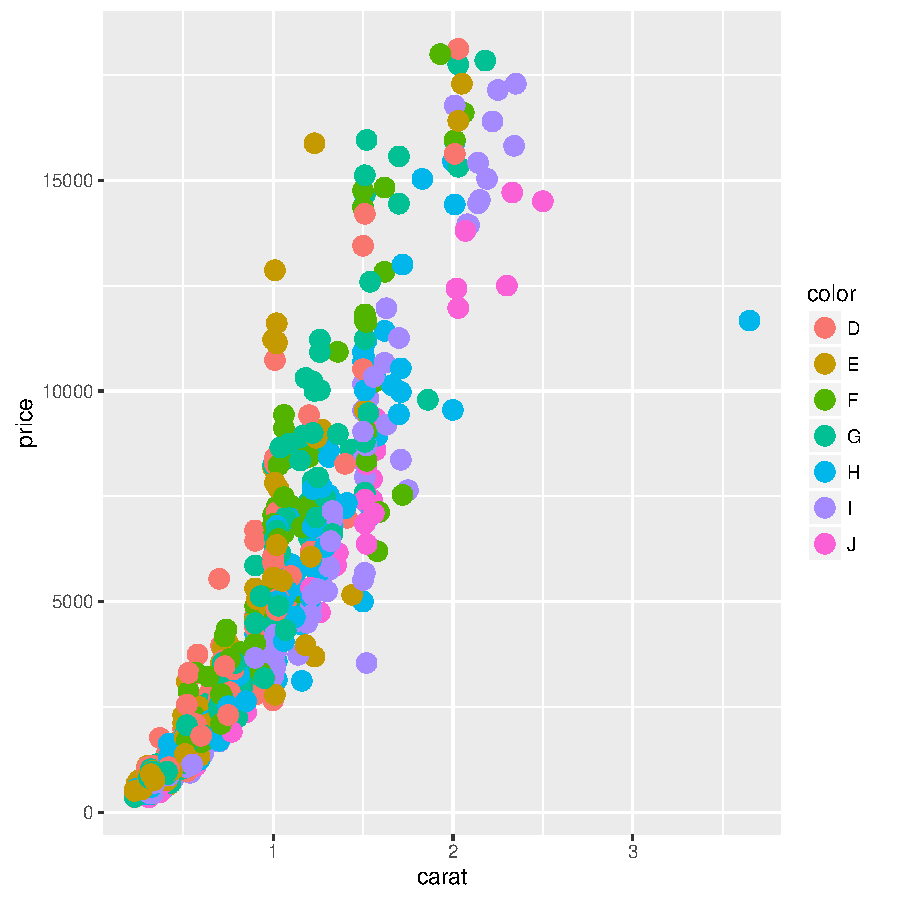
\includegraphics{fig--044}
\label{fig:qplotscatter}
\end{figure}
\end{frame}
%%%%%%%%%%%%%%%%%%%%%%%%%%%%%%%%% slide %%%%%%%%%%%%%%%%%%%%%%%%%%%%%%%%%
\begin{frame}[containsverbatim]  
	\frametitle{ggplot: Scatter Plot with Regression Line}
\scriptsize 
\begin{figure}
  \centering
\begin{Schunk}
\begin{Sinput}
> p <- ggplot(dsmall, aes(carat, price)) + geom_point() + 
+             geom_smooth(method="lm", se=FALSE) +
+ 	    theme(panel.background=element_rect(fill = "white", colour = "black"))
> print(p) 
\end{Sinput}
\end{Schunk}
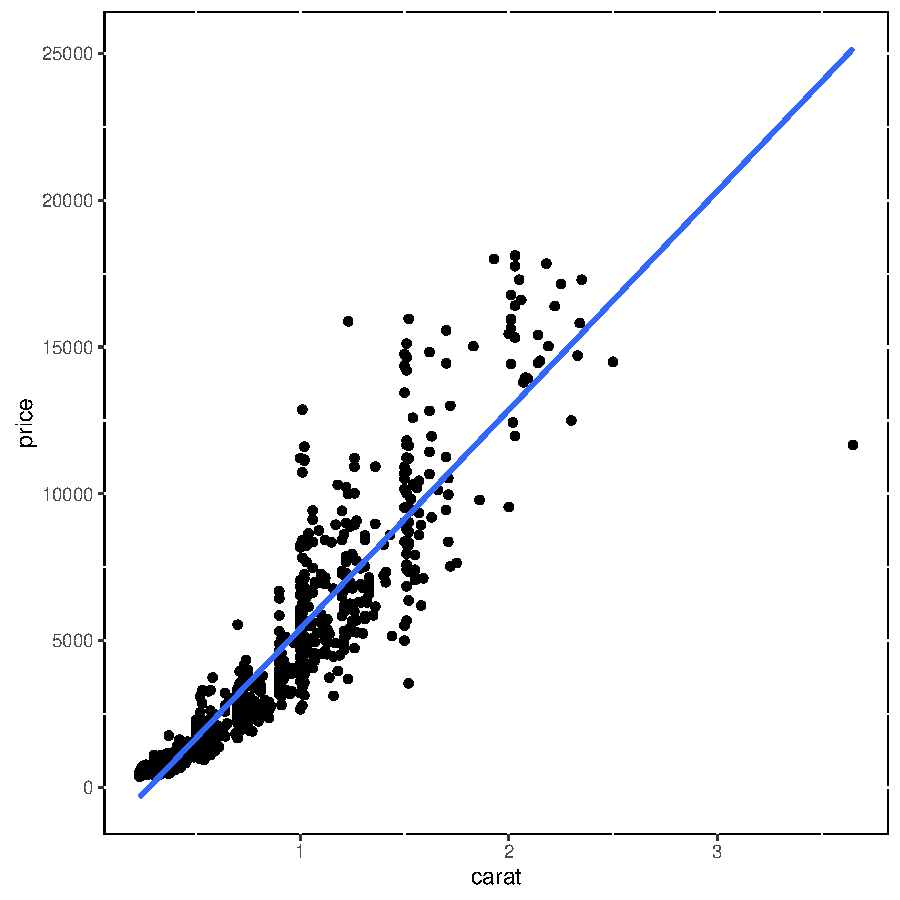
\includegraphics{fig--045}
\label{fig:qplotscatter}
\end{figure}
\end{frame}
%%%%%%%%%%%%%%%%%%%%%%%%%%%%%%%%% slide %%%%%%%%%%%%%%%%%%%%%%%%%%%%%%%%%
\begin{frame}[containsverbatim]  
	\frametitle{ggplot: Scatter Plot with Several Regression Lines}
\scriptsize 
\begin{figure}
  \centering
\begin{Schunk}
\begin{Sinput}
> p <- ggplot(dsmall, aes(carat, price, group=color)) + 
+             geom_point(aes(color=color), size=2) + 
+             geom_smooth(aes(color=color), method = "lm", se=FALSE) 
> print(p) 
\end{Sinput}
\end{Schunk}
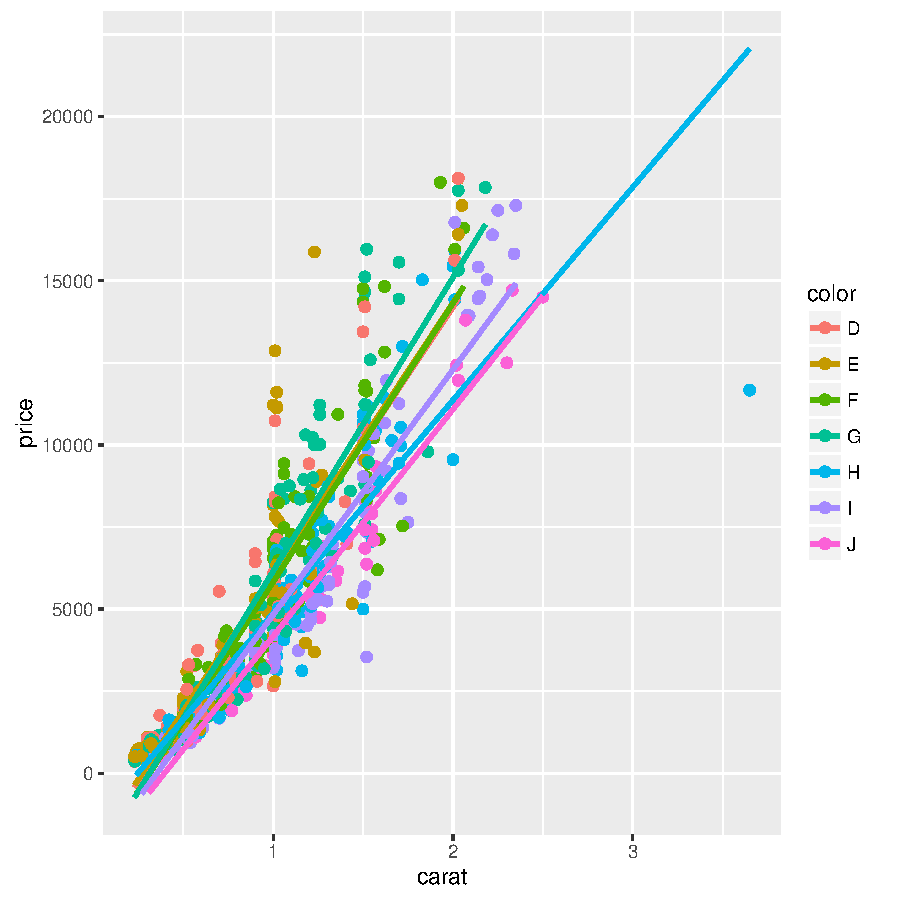
\includegraphics{fig--046}
\label{fig:qplotscatter}
\end{figure}
\end{frame}
%%%%%%%%%%%%%%%%%%%%%%%%%%%%%%%%% slide %%%%%%%%%%%%%%%%%%%%%%%%%%%%%%%%%
\begin{frame}[containsverbatim]  
	\frametitle{ggplot: Scatter Plot with Local Regression Curve (loess)}
\scriptsize 
\begin{figure}
  \centering
\begin{Schunk}
\begin{Sinput}
> p <- ggplot(dsmall, aes(carat, price)) + geom_point() + geom_smooth() 
> print(p) # Setting se=FALSE removes error shade
\end{Sinput}
\end{Schunk}
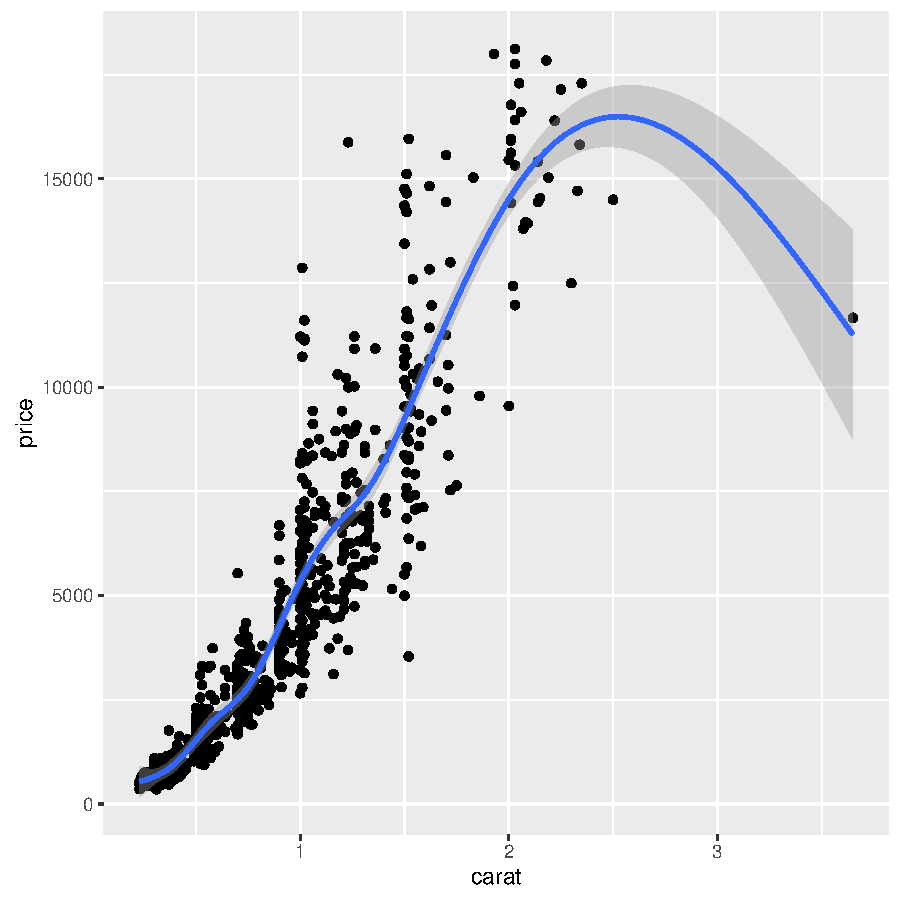
\includegraphics{fig--047}
\label{fig:qplotscatter}
\end{figure}
\end{frame}
%%%%%%%%%%%%%%%%%%%%%%%%%%%%%%%%% slide %%%%%%%%%%%%%%%%%%%%%%%%%%%%%%%%%
\begin{frame}[containsverbatim]  
	\frametitle{ggplot: Line Plot}
\scriptsize 
\begin{figure}
  \centering
\begin{Schunk}
\begin{Sinput}
> p <- ggplot(iris, aes(Petal.Length, Petal.Width, group=Species, 
+             color=Species)) + geom_line() 
> print(p) 
\end{Sinput}
\end{Schunk}
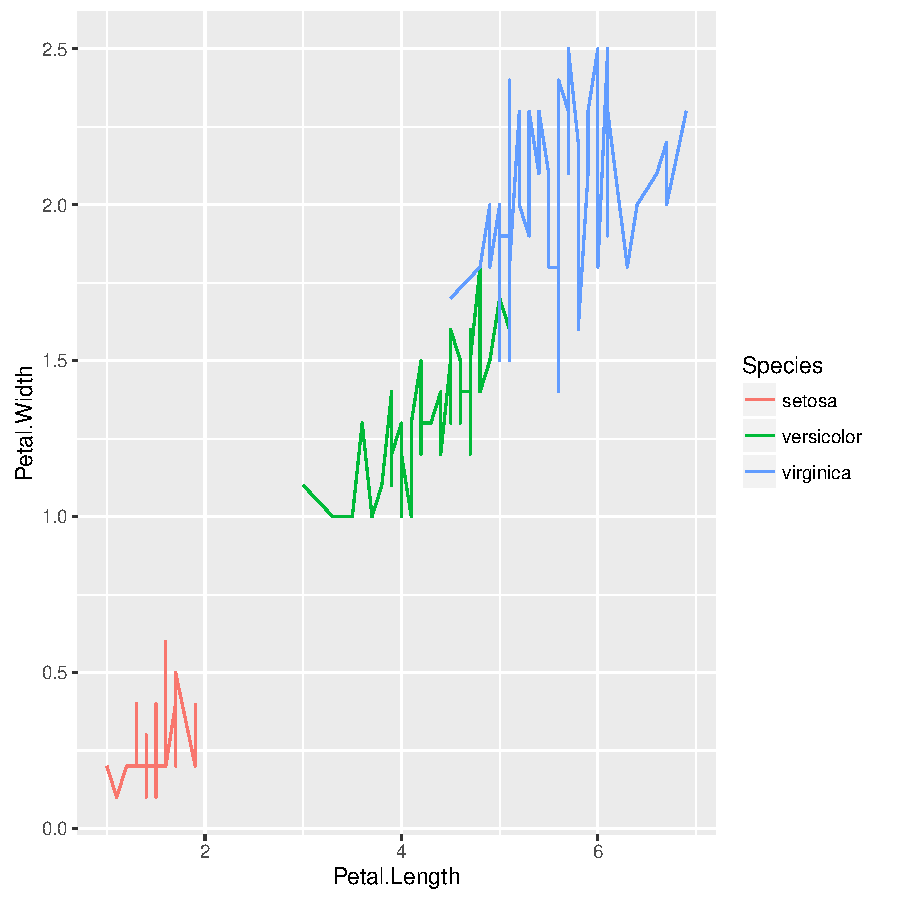
\includegraphics{fig--048}
\label{fig:qplotscatter}
\end{figure}
\end{frame}
%%%%%%%%%%%%%%%%%%%%%%%%%%%%%%%%% slide %%%%%%%%%%%%%%%%%%%%%%%%%%%%%%%%%
\begin{frame}[containsverbatim]  
	\frametitle{ggplot: Faceting}
\scriptsize 
\begin{figure}
  \centering
\begin{Schunk}
\begin{Sinput}
> p <- ggplot(iris, aes(Sepal.Length, Sepal.Width)) + 
+ 	    geom_line(aes(color=Species), size=1) + 
+             facet_wrap(~Species, ncol=1)
> print(p) 
\end{Sinput}
\end{Schunk}
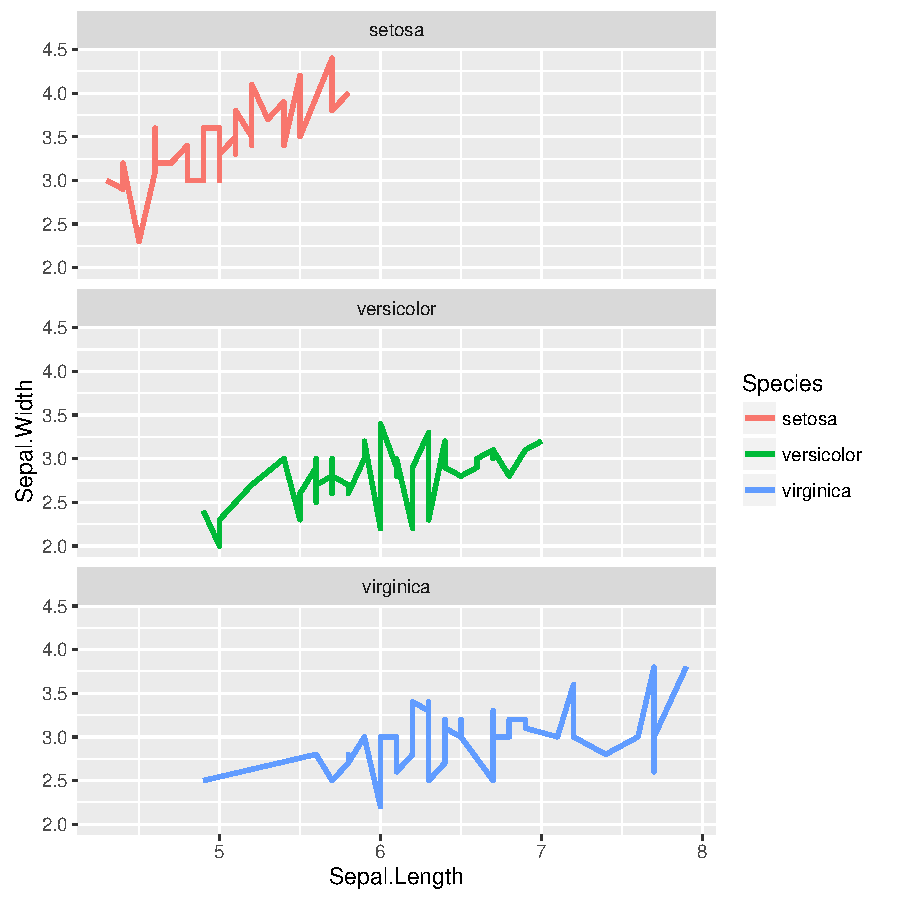
\includegraphics{fig--049}
\label{fig:qplotscatter}
\end{figure}
\end{frame}
%%%%%%%%%%%%%%%%%%%%%%%%%%%%%%%%% SLIDE %%%%%%%%%%%%%%%%%%%%%%%%%%%%%%%%%
\begin{frame}[containsverbatim]  
	\frametitle{Exercise 3: Scatter Plots}
\scriptsize
\begin{itemize}
        \item[Task 1] Generate scatter plot for first two columns in \Rfunction{iris} data frame and color dots by its \Rfunction{Species} column.
        \item[Task 2] Use the \Rfunarg{xlim, ylim} functionss to set limits on the x- and y-axes so that all data points are restricted to the left bottom quadrant of the plot. 
        \item[Task 3] Generate corresponding line plot with faceting show individual data sets in saparate plots. 
        \item[]\hspace{-1.1cm} Structure of iris data set:
\end{itemize}
\begin{Schunk}
\begin{Sinput}
> class(iris)
\end{Sinput}
\begin{Soutput}
[1] "data.frame"
\end{Soutput}
\begin{Sinput}
> iris[1:4,]
\end{Sinput}
\begin{Soutput}
  Sepal.Length Sepal.Width Petal.Length Petal.Width Species
1          5.1         3.5          1.4         0.2  setosa
2          4.9         3.0          1.4         0.2  setosa
3          4.7         3.2          1.3         0.2  setosa
4          4.6         3.1          1.5         0.2  setosa
\end{Soutput}
\begin{Sinput}
> table(iris$Species)
\end{Sinput}
\begin{Soutput}
    setosa versicolor  virginica 
        50         50         50 
\end{Soutput}
\end{Schunk}
\end{frame}
%%%%%%%%%%%%%%%%%%%%%%%%%%%%%%%%% slide %%%%%%%%%%%%%%%%%%%%%%%%%%%%%%%%%
\begin{frame}[containsverbatim]  
	\frametitle{ggplot: Bar Plots}
\vspace{0cm}
\begin{changemargin}{-0.6cm}{-0.8cm}
\scriptsize 
\textcolor{blue}{\textbf{Sample Set}: the following transforms the iris data set into a ggplot2-friendly format.}

\vspace{0.2cm}
\textcolor{blue}{Calculate mean values for aggregates given by \Robject{Species} column in iris data set}
\begin{Schunk}
\begin{Sinput}
> iris_mean <- aggregate(iris[,1:4], by=list(Species=iris$Species), FUN=mean) 
\end{Sinput}
\end{Schunk}

\textcolor{blue}{Calculate standard deviations for aggregates given by \Robject{Species} column in \Robject{iris} data set}
\begin{Schunk}
\begin{Sinput}
> iris_sd <- aggregate(iris[,1:4], by=list(Species=iris$Species), FUN=sd) 
\end{Sinput}
\end{Schunk}

\textcolor{blue}{Convert \Robject{iris\_mean} with \Rfunction{melt}}
\begin{Schunk}
\begin{Sinput}
> library(reshape2) # Defines melt function
> df_mean <- melt(iris_mean, id.vars=c("Species"), variable.name = "Samples", value.name="Values")
\end{Sinput}
\end{Schunk}

\textcolor{blue}{Convert \Robject{iris\_sd} with \Rfunction{melt}}
\begin{Schunk}
\begin{Sinput}
> df_sd <- melt(iris_sd, id.vars=c("Species"), variable.name = "Samples", value.name="Values")
\end{Sinput}
\end{Schunk}

\textcolor{blue}{Define standard deviation limits}
\begin{Schunk}
\begin{Sinput}
> limits <- aes(ymax = df_mean[,"Values"] + df_sd[,"Values"], ymin=df_mean[,"Values"] - df_sd[,"Values"])
\end{Sinput}
\end{Schunk}
\end{changemargin}
\end{frame}
%%%%%%%%%%%%%%%%%%%%%%%%%%%%%%%%% slide %%%%%%%%%%%%%%%%%%%%%%%%%%%%%%%%%
\begin{frame}[containsverbatim]  
	\frametitle{ggplot: Bar Plot}
\scriptsize 
\begin{figure}
  \centering
\begin{Schunk}
\begin{Sinput}
> p <- ggplot(df_mean, aes(Samples, Values, fill = Species)) + 
+ 	    geom_bar(position="dodge", stat="identity")
> print(p) 
\end{Sinput}
\end{Schunk}
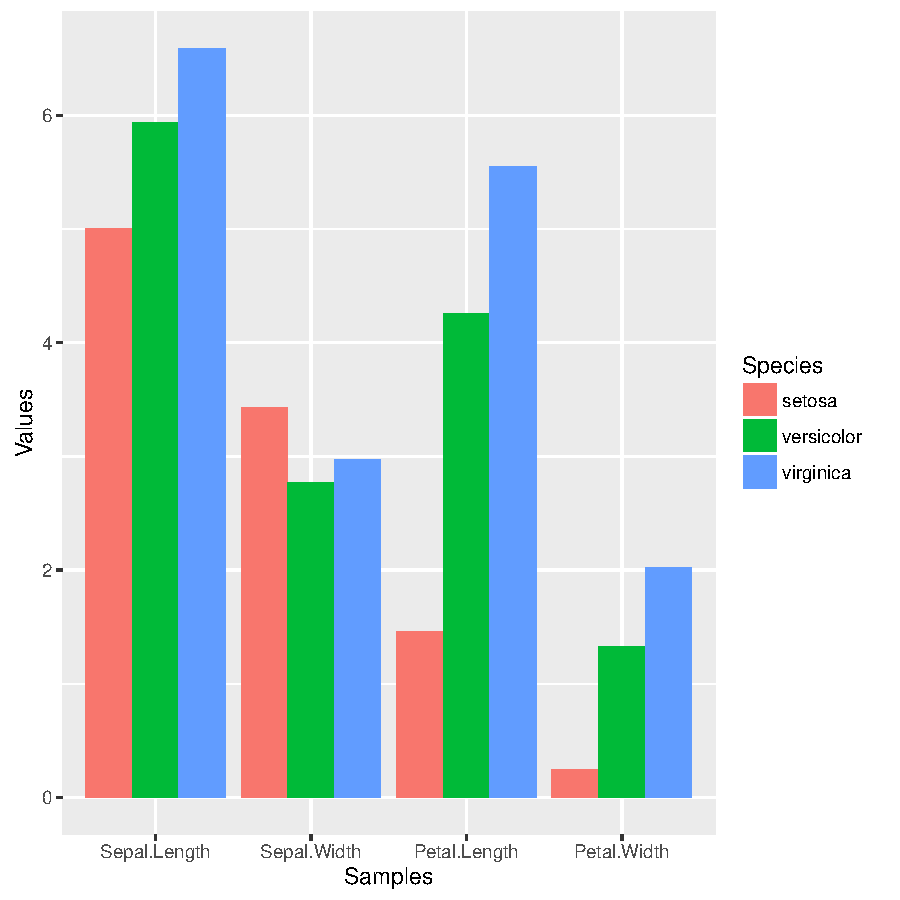
\includegraphics{fig--057}
\label{fig:qplotscatter}
\end{figure}
\end{frame}
%%%%%%%%%%%%%%%%%%%%%%%%%%%%%%%%% slide %%%%%%%%%%%%%%%%%%%%%%%%%%%%%%%%%
\begin{frame}[containsverbatim]  
	\frametitle{ggplot: Bar Plot Sideways}
\scriptsize 
\begin{figure}
  \centering
\begin{Schunk}
\begin{Sinput}
> p <- ggplot(df_mean, aes(Samples, Values, fill = Species)) + 
+             geom_bar(position="dodge", stat="identity") + coord_flip() + 
+             theme(axis.text.y=element_text(angle=0, hjust=1))
> print(p) 
\end{Sinput}
\end{Schunk}
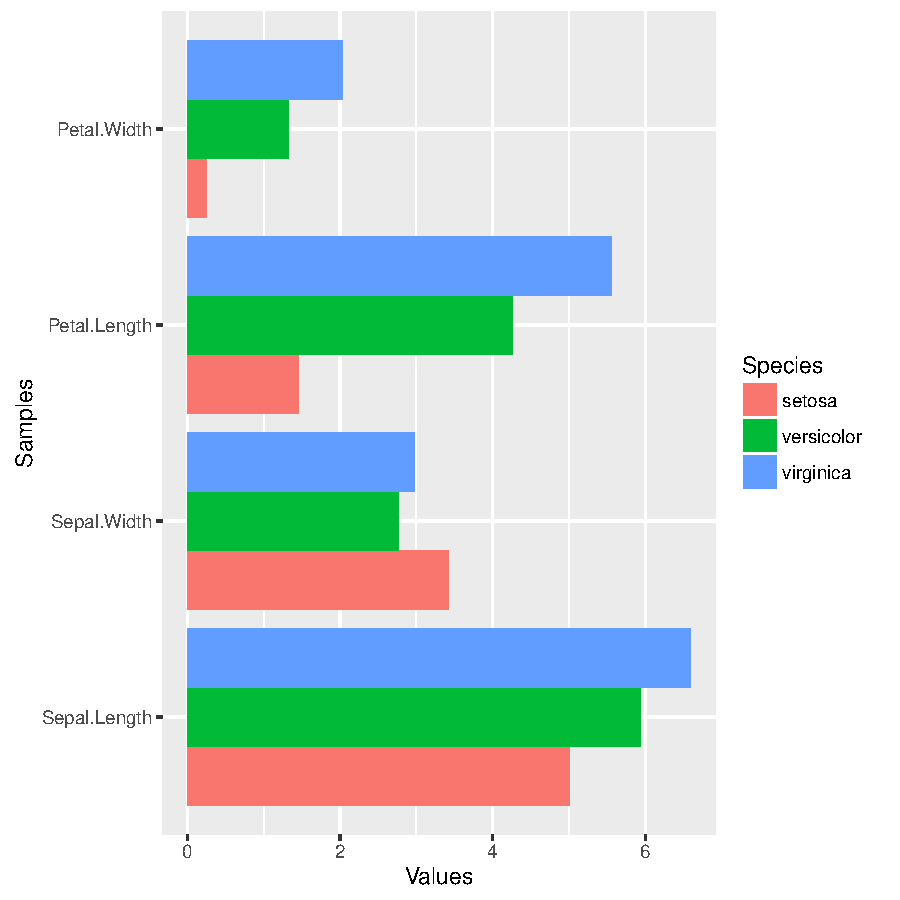
\includegraphics{fig--058}
\label{fig:qplotscatter}
\end{figure}
\end{frame}
%%%%%%%%%%%%%%%%%%%%%%%%%%%%%%%%% slide %%%%%%%%%%%%%%%%%%%%%%%%%%%%%%%%%
\begin{frame}[containsverbatim]  
	\frametitle{ggplot: Bar Plot with Faceting}
\scriptsize 
\begin{figure}
  \centering
\begin{Schunk}
\begin{Sinput}
> p <- ggplot(df_mean, aes(Samples, Values)) + geom_bar(aes(fill = Species), stat="identity") + 
+             facet_wrap(~Species, ncol=1)
> print(p) 
\end{Sinput}
\end{Schunk}
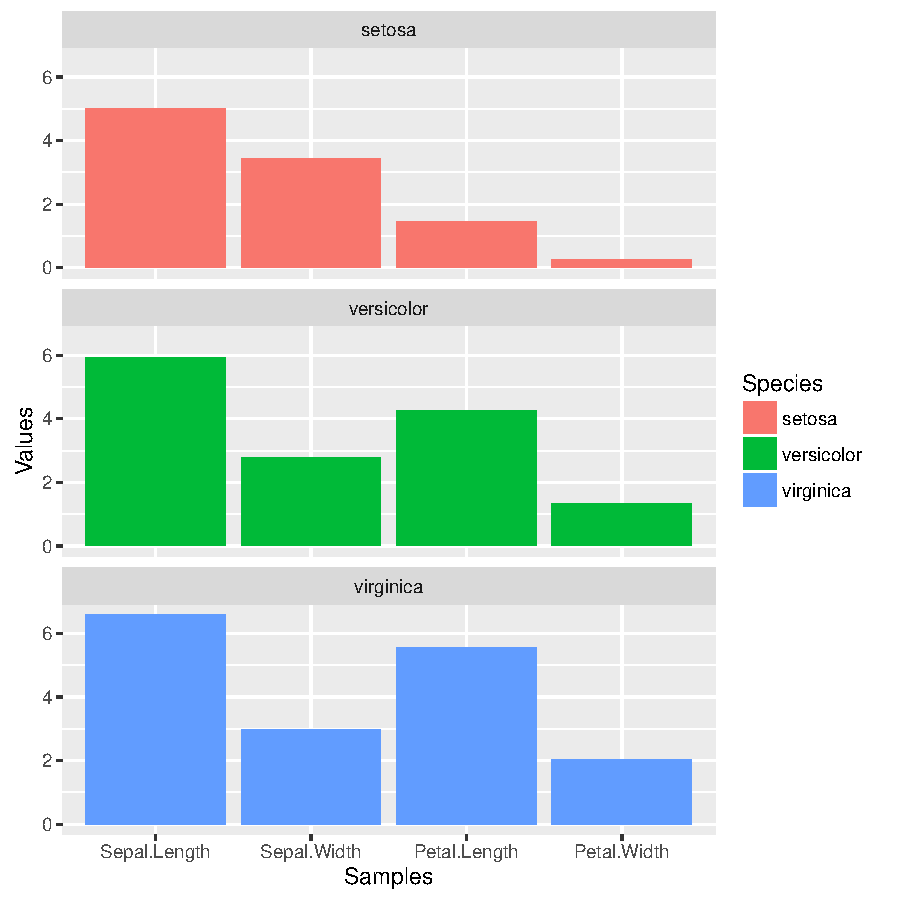
\includegraphics{fig--059}
\label{fig:qplotscatter}
\end{figure}
\end{frame}
%%%%%%%%%%%%%%%%%%%%%%%%%%%%%%%%% slide %%%%%%%%%%%%%%%%%%%%%%%%%%%%%%%%%
\begin{frame}[containsverbatim]  
	\frametitle{ggplot: Bar Plot with Error Bars}
\scriptsize 
\begin{figure}
  \centering
\begin{Schunk}
\begin{Sinput}
> p <- ggplot(df_mean, aes(Samples, Values, fill = Species)) + 
+ 	    geom_bar(position="dodge", stat="identity") + geom_errorbar(limits, position="dodge") 
> print(p) 
\end{Sinput}
\end{Schunk}
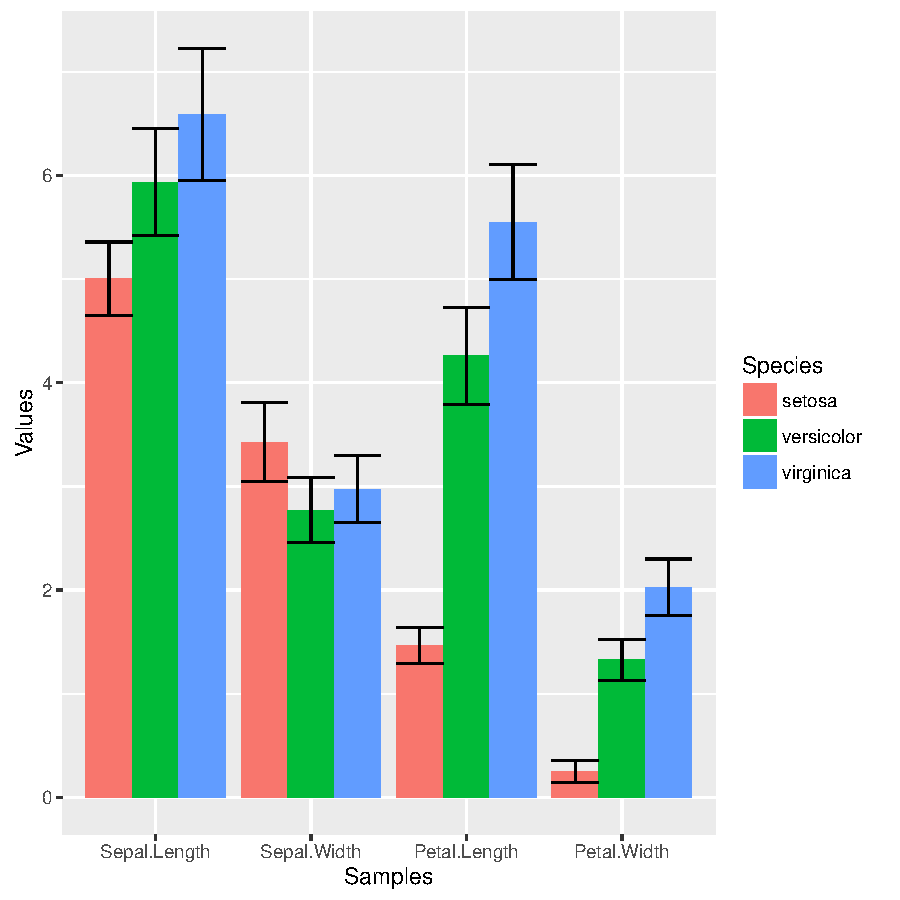
\includegraphics{fig--060}
\label{fig:qplotscatter}
\end{figure}
\end{frame}
%%%%%%%%%%%%%%%%%%%%%%%%%%%%%%%%% slide %%%%%%%%%%%%%%%%%%%%%%%%%%%%%%%%%
\begin{frame}[containsverbatim]  
	\frametitle{ggplot: Changing Color Settings}
\tiny
\begin{figure}
  \centering
\begin{Schunk}
\begin{Sinput}
> library(RColorBrewer)
> # display.brewer.all() 
> p <- ggplot(df_mean, aes(Samples, Values, fill=Species, color=Species)) +
+             geom_bar(position="dodge", stat="identity") + geom_errorbar(limits, position="dodge") + 
+             scale_fill_brewer(palette="Blues") + scale_color_brewer(palette = "Greys") 
> print(p) 
\end{Sinput}
\end{Schunk}
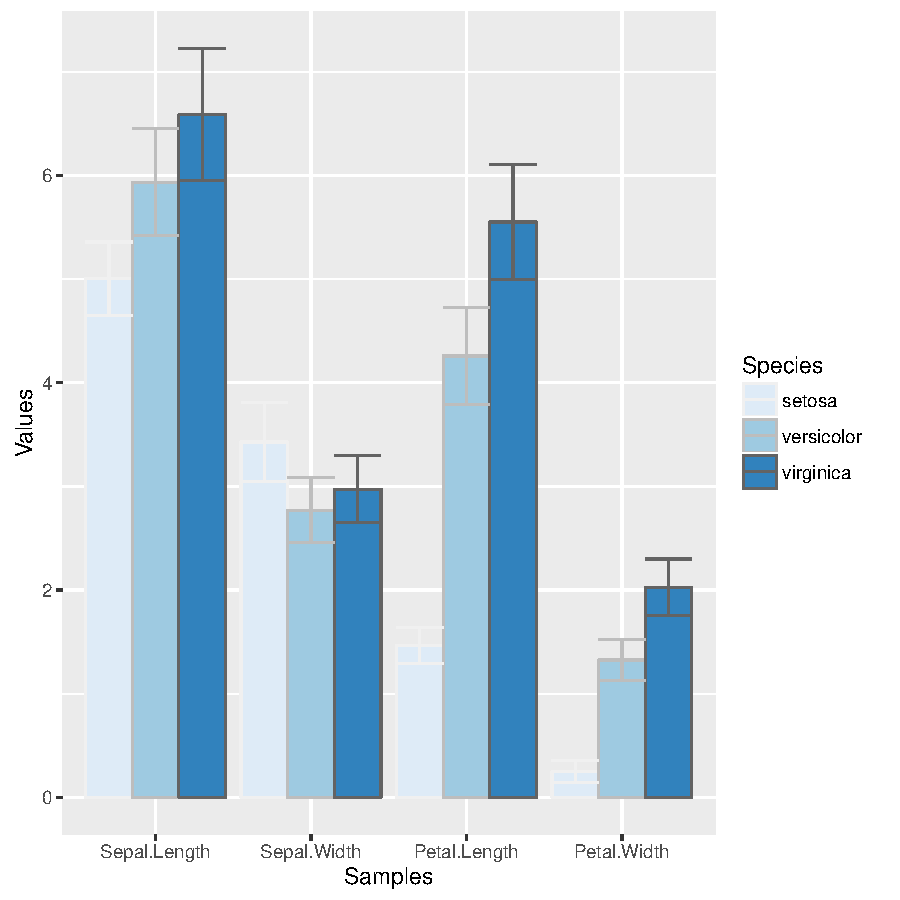
\includegraphics{fig--061}
\label{fig:qplotscatter}
\end{figure}
\end{frame}
%%%%%%%%%%%%%%%%%%%%%%%%%%%%%%%%% slide %%%%%%%%%%%%%%%%%%%%%%%%%%%%%%%%%
\begin{frame}[containsverbatim]  
	\frametitle{ggplot: Using Standard Colors}
\tiny
\begin{figure}
  \centering
\begin{Schunk}
\begin{Sinput}
> p <- ggplot(df_mean, aes(Samples, Values, fill=Species, color=Species)) + 
+             geom_bar(position="dodge", stat="identity") + geom_errorbar(limits, position="dodge") + 
+             scale_fill_manual(values=c("red", "green3", "blue")) + 
+             scale_color_manual(values=c("red", "green3", "blue")) 
> print(p) 
\end{Sinput}
\end{Schunk}
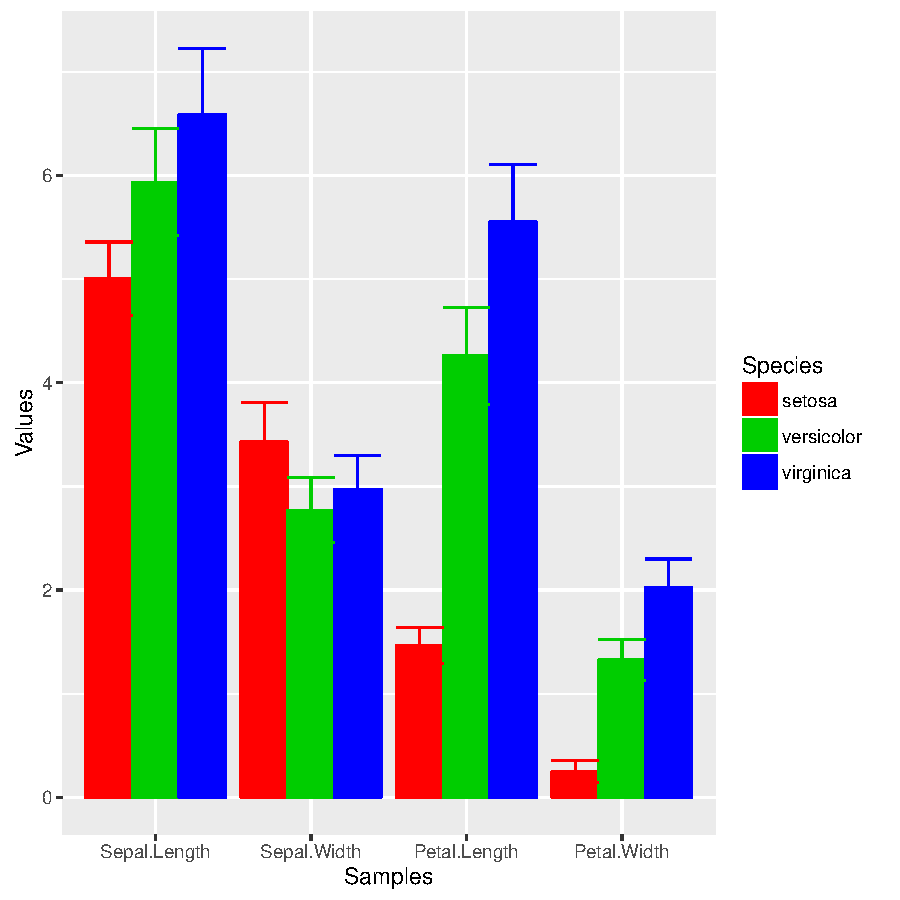
\includegraphics{fig--062}
\label{fig:qplotscatter}
\end{figure}
\end{frame}
%%%%%%%%%%%%%%%%%%%%%%%%%%%%%%%%% slide %%%%%%%%%%%%%%%%%%%%%%%%%%%%%%%%%
\begin{frame}[containsverbatim]  
	\frametitle{ggplot: Mirrored Bar Plots}
\tiny
\begin{figure}
  \centering
\begin{Schunk}
\begin{Sinput}
> df <- data.frame(group = rep(c("Above", "Below"), each=10), x = rep(1:10, 2), y = c(runif(10, 0, 1), runif(10, -1, 0)))
> p <- ggplot(df, aes(x=x, y=y, fill=group)) + 
+ 	    geom_bar(stat="identity", position="identity")
> print(p) 
\end{Sinput}
\end{Schunk}
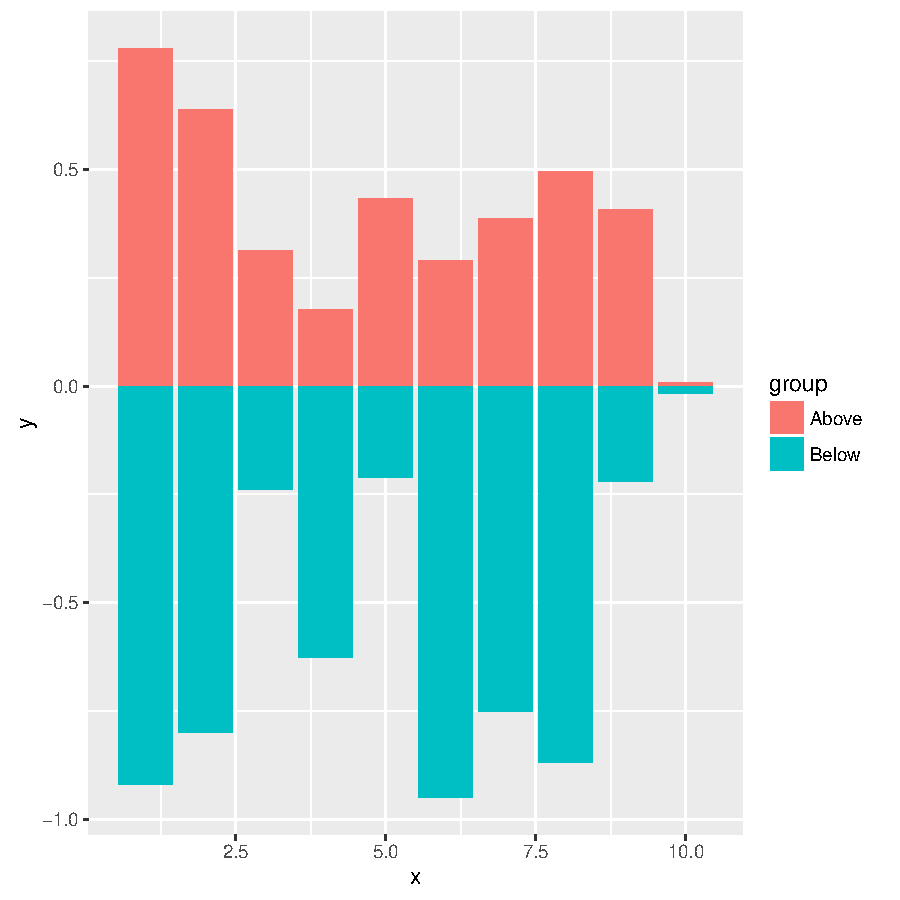
\includegraphics{fig--063}
\label{fig:qplotscatter}
\end{figure}
\end{frame}
%%%%%%%%%%%%%%%%%%%%%%%%%%%%%%%%% SLIDE %%%%%%%%%%%%%%%%%%%%%%%%%%%%%%%%%
\begin{frame}[containsverbatim]  
	\frametitle{Exercise 4: Bar Plots}
\scriptsize
\begin{itemize}
        \item[Task 1] Calculate the mean values for the \Rfunction{Species} components of the first four columns in the \Rfunction{iris} data set. Use the \Rfunction{melt} function from the \Rpackage{reshape2} package to bring the results into the expected format for \Rfunction{ggplot}.
        \item[Task 2] Generate two bar plots: one with stacked bars and one with horizontally arranged bars. 
        \item[]\hspace{-1.1cm} Structure of iris data set:
\end{itemize}
\begin{Schunk}
\begin{Sinput}
> class(iris)
\end{Sinput}
\begin{Soutput}
[1] "data.frame"
\end{Soutput}
\begin{Sinput}
> iris[1:4,]
\end{Sinput}
\begin{Soutput}
  Sepal.Length Sepal.Width Petal.Length Petal.Width Species
1          5.1         3.5          1.4         0.2  setosa
2          4.9         3.0          1.4         0.2  setosa
3          4.7         3.2          1.3         0.2  setosa
4          4.6         3.1          1.5         0.2  setosa
\end{Soutput}
\begin{Sinput}
> table(iris$Species)
\end{Sinput}
\begin{Soutput}
    setosa versicolor  virginica 
        50         50         50 
\end{Soutput}
\end{Schunk}
\end{frame}
%%%%%%%%%%%%%%%%%%%%%%%%%%%%%%%%% slide %%%%%%%%%%%%%%%%%%%%%%%%%%%%%%%%%
\begin{frame}[containsverbatim]  
	\frametitle{ggplot: Data Reformatting Example for Line Plot}
\tiny
\begin{figure}
  \centering
\begin{Schunk}
\begin{Sinput}
> y <- matrix(rnorm(500), 100, 5, dimnames=list(paste("g", 1:100, sep=""), paste("Sample", 1:5, sep="")))
> y <- data.frame(Position=1:length(y[,1]), y)
> y[1:4, ] # First rows of input format expected by melt()
\end{Sinput}
\begin{Soutput}
   Position    Sample1    Sample2     Sample3     Sample4    Sample5
g1        1  1.0002088  0.6850199 -0.21324932  1.27195056  1.0479301
g2        2 -1.2024596 -1.5004962 -0.01111579  0.07584497 -0.7100662
g3        3  0.1023678 -0.5153367  0.28564390  1.41522878  1.1084695
g4        4  1.3294248 -1.2084007 -0.19581898 -0.42361768  1.7139697
\end{Soutput}
\begin{Sinput}
> df <- melt(y, id.vars=c("Position"), variable.name = "Samples", value.name="Values")
> p <- ggplot(df, aes(Position, Values)) + geom_line(aes(color=Samples)) + facet_wrap(~Samples, ncol=1)
> print(p)
> ## Represent same data in box plot
> ## ggplot(df, aes(Samples, Values, fill=Samples)) + geom_boxplot()
\end{Sinput}
\end{Schunk}
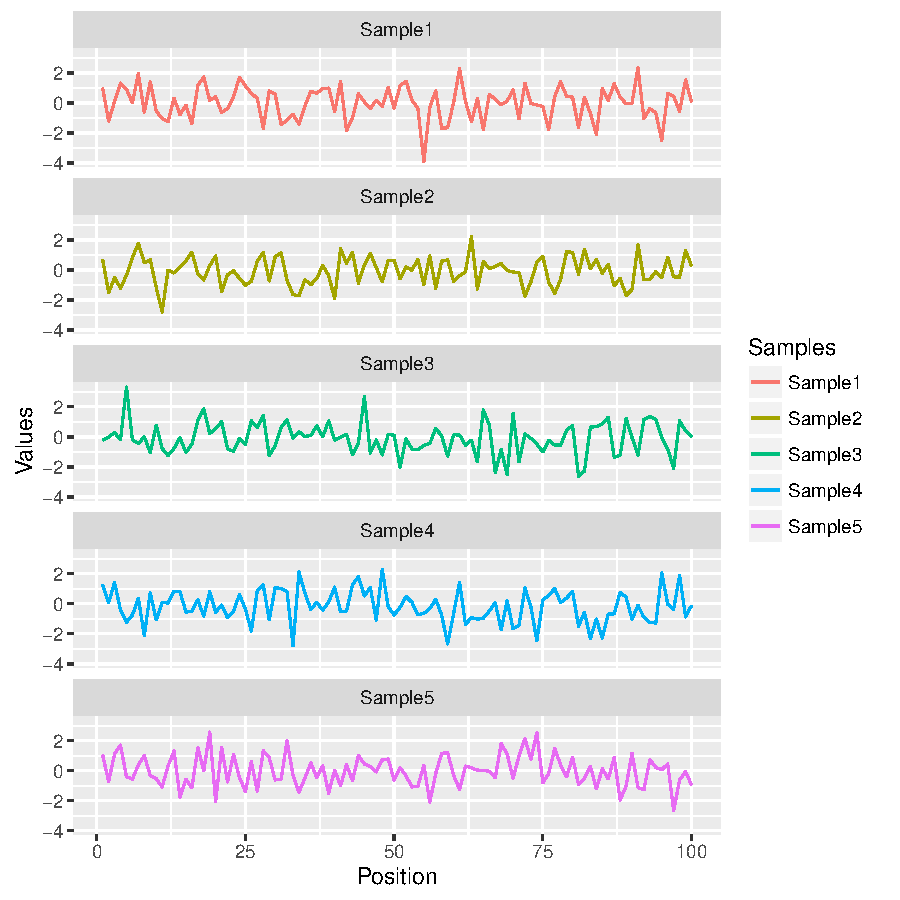
\includegraphics{fig--066}
\label{fig:lineplot_split}
\end{figure}
\end{frame}
%%%%%%%%%%%%%%%%%%%%%%%%%%%%%%%%% slide %%%%%%%%%%%%%%%%%%%%%%%%%%%%%%%%%
\begin{frame}[containsverbatim]  
	\frametitle{ggplot: Jitter Plots}
\scriptsize 
\begin{figure}
  \centering
\begin{Schunk}
\begin{Sinput}
> p <- ggplot(dsmall, aes(color, price/carat)) + 
+             geom_jitter(alpha = I(1 / 2), aes(color=color))
> print(p) 
\end{Sinput}
\end{Schunk}
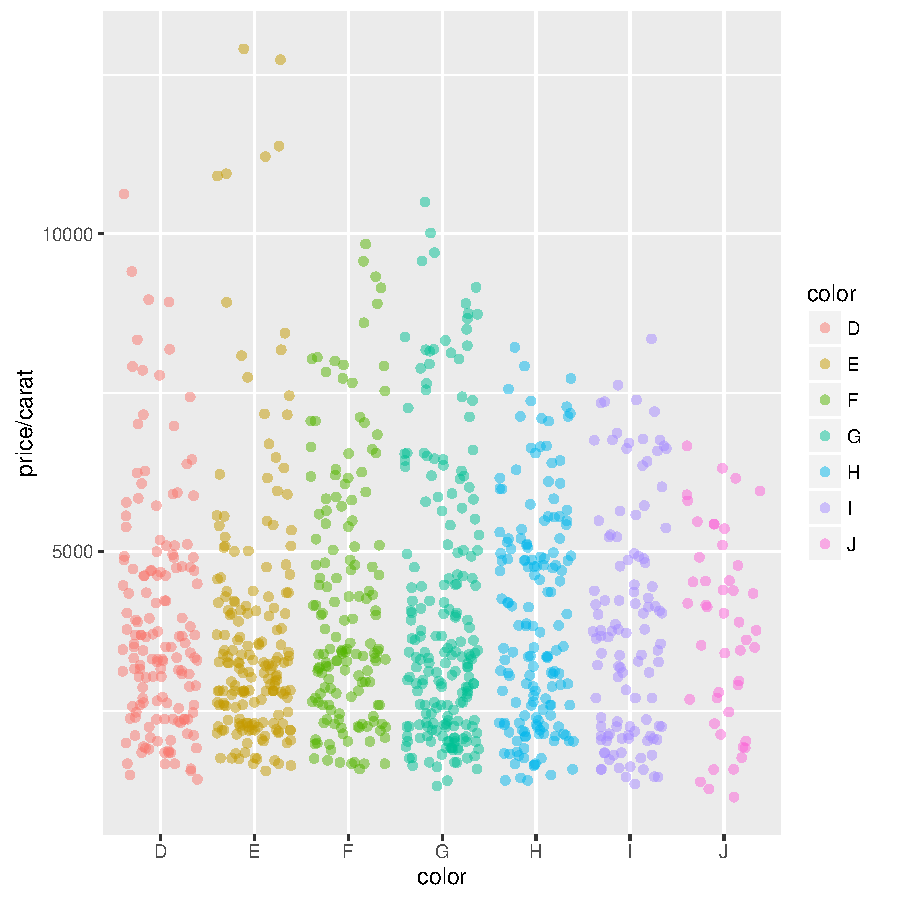
\includegraphics{fig--067}
\label{fig:qplotscatter}
\end{figure}
\end{frame}
%%%%%%%%%%%%%%%%%%%%%%%%%%%%%%%%% slide %%%%%%%%%%%%%%%%%%%%%%%%%%%%%%%%%
\begin{frame}[containsverbatim]  
	\frametitle{ggplot: Box Plots}
\scriptsize 
\begin{figure}
  \centering
\begin{Schunk}
\begin{Sinput}
> p <- ggplot(dsmall, aes(color, price/carat, fill=color)) + geom_boxplot()
> print(p) 
\end{Sinput}
\end{Schunk}
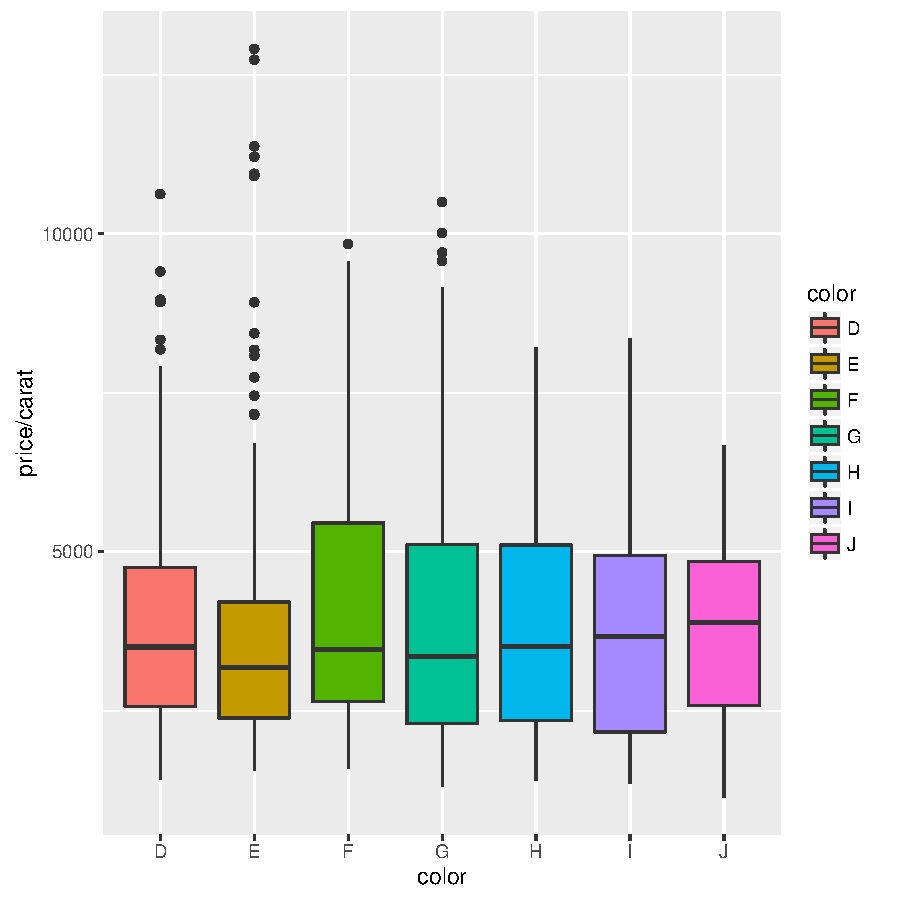
\includegraphics{fig--068}
\label{fig:qplotscatter}
\end{figure}
\end{frame}
%%%%%%%%%%%%%%%%%%%%%%%%%%%%%%%%% slide %%%%%%%%%%%%%%%%%%%%%%%%%%%%%%%%%
\begin{frame}[containsverbatim]  
	\frametitle{ggplot: Density Plot with Line Coloring}
\scriptsize 
\begin{figure}
  \centering
\begin{Schunk}
\begin{Sinput}
> p <- ggplot(dsmall, aes(carat)) + geom_density(aes(color = color))
> print(p) 
\end{Sinput}
\end{Schunk}
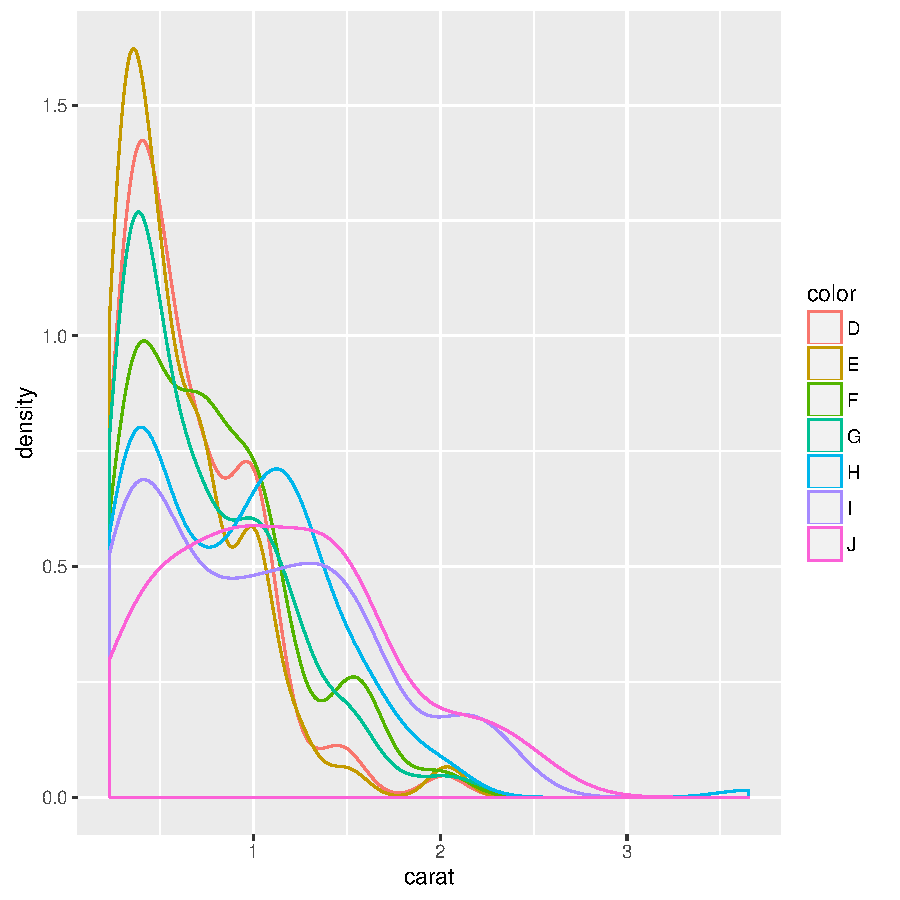
\includegraphics{fig--069}
\label{fig:qplotscatter}
\end{figure}
\end{frame}
%%%%%%%%%%%%%%%%%%%%%%%%%%%%%%%%% slide %%%%%%%%%%%%%%%%%%%%%%%%%%%%%%%%%
\begin{frame}[containsverbatim]  
	\frametitle{ggplot: Density Plot with Area Coloring}
\scriptsize 
\begin{figure}
  \centering
\begin{Schunk}
\begin{Sinput}
> p <- ggplot(dsmall, aes(carat)) + geom_density(aes(fill = color))
> print(p) 
\end{Sinput}
\end{Schunk}
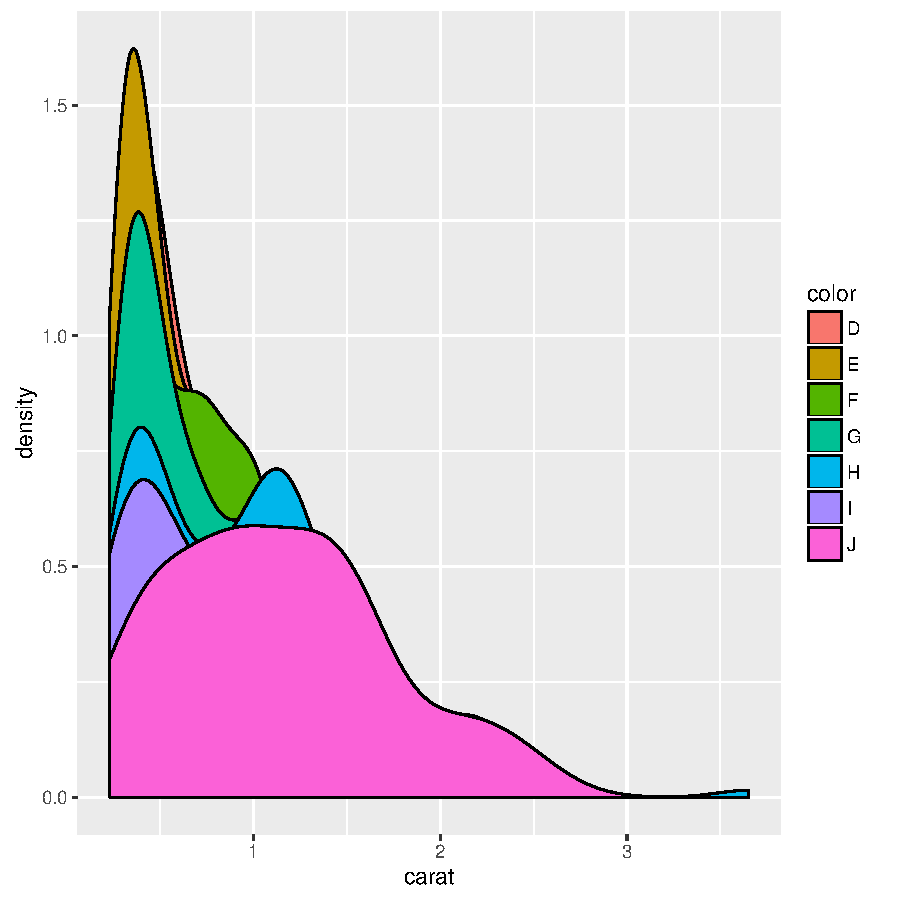
\includegraphics{fig--070}
\label{fig:qplotscatter}
\end{figure}
\end{frame}
%%%%%%%%%%%%%%%%%%%%%%%%%%%%%%%%% slide %%%%%%%%%%%%%%%%%%%%%%%%%%%%%%%%%
\begin{frame}[containsverbatim]  
	\frametitle{ggplot: Histograms}
\scriptsize 
\begin{figure}
  \centering
\begin{Schunk}
\begin{Sinput}
> p <- ggplot(iris, aes(x=Sepal.Width)) + geom_histogram(aes(y = ..density.., 
+             fill = ..count..), binwidth=0.2) + geom_density()  
> print(p) 
\end{Sinput}
\end{Schunk}
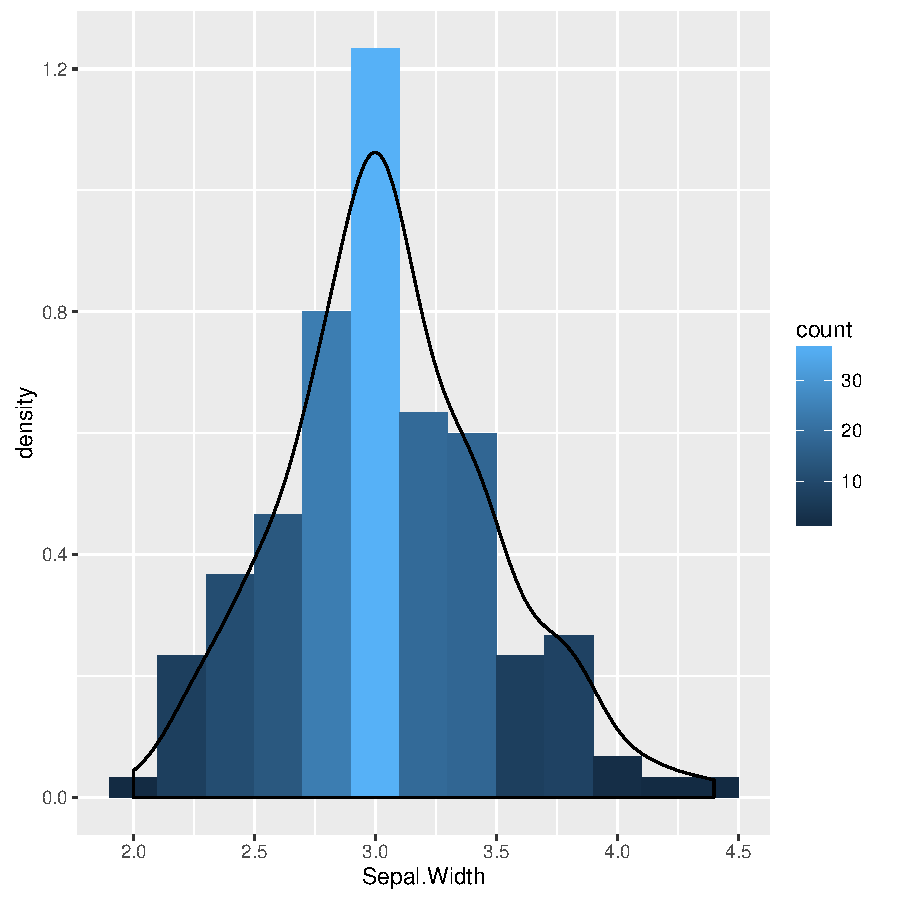
\includegraphics{fig--071}
\label{fig:qplotscatter}
\end{figure}
\end{frame}
%%%%%%%%%%%%%%%%%%%%%%%%%%%%%%%%% slide %%%%%%%%%%%%%%%%%%%%%%%%%%%%%%%%%
\begin{frame}[containsverbatim]  
	\frametitle{ggplot: Pie Chart}
\scriptsize 
\begin{figure}
  \centering
\begin{Schunk}
\begin{Sinput}
> df <- data.frame(variable=rep(c("cat", "mouse", "dog", "bird", "fly")), 
+                  value=c(1,3,3,4,2)) 
> p <- ggplot(df, aes(x = "", y = value, fill = variable)) + 
+             geom_bar(width = 1, stat="identity") + 
+             coord_polar("y", start=pi / 3) + ggtitle("Pie Chart") 
> print(p) 
\end{Sinput}
\end{Schunk}
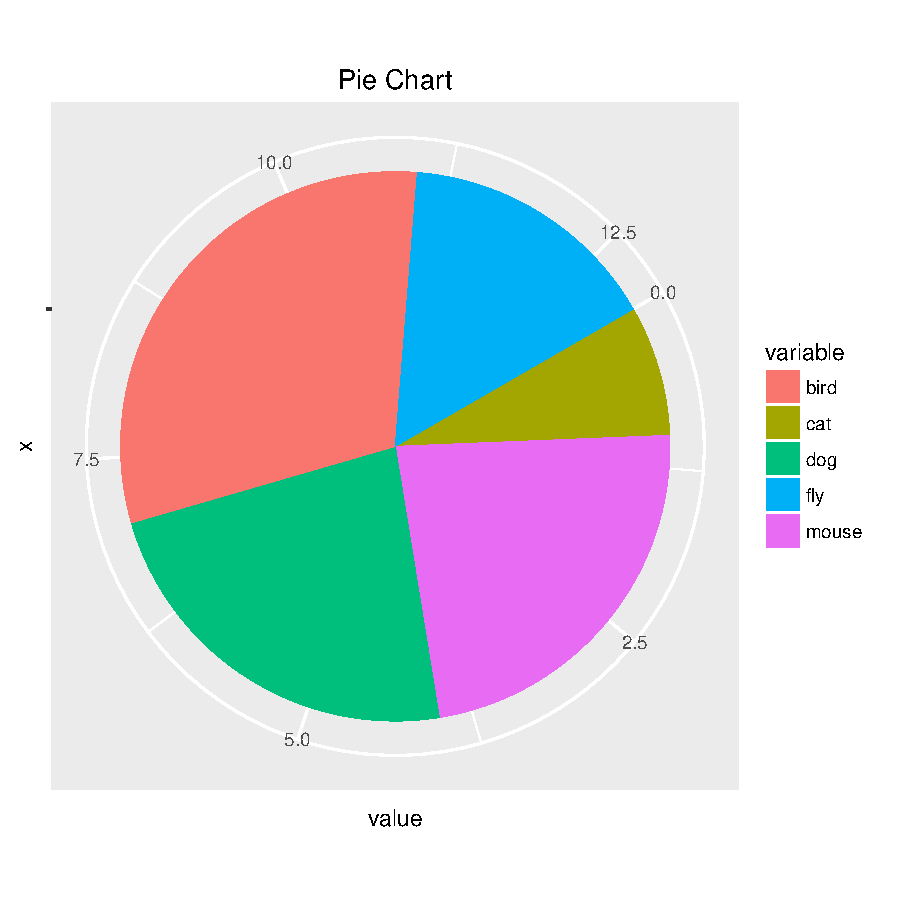
\includegraphics{fig--072}
\label{fig:qplotscatter}
\end{figure}
\end{frame}
%%%%%%%%%%%%%%%%%%%%%%%%%%%%%%%%% slide %%%%%%%%%%%%%%%%%%%%%%%%%%%%%%%%%
\begin{frame}[containsverbatim]  
	\frametitle{ggplot: Wind Rose Pie Chart}
\scriptsize 
\begin{figure}
  \centering
\begin{Schunk}
\begin{Sinput}
> p <- ggplot(df, aes(x = variable, y = value, fill = variable)) + 
+        geom_bar(width = 1, stat="identity") + coord_polar("y", start=pi / 3) + 
+        ggtitle("Pie Chart") 
> print(p) 
\end{Sinput}
\end{Schunk}
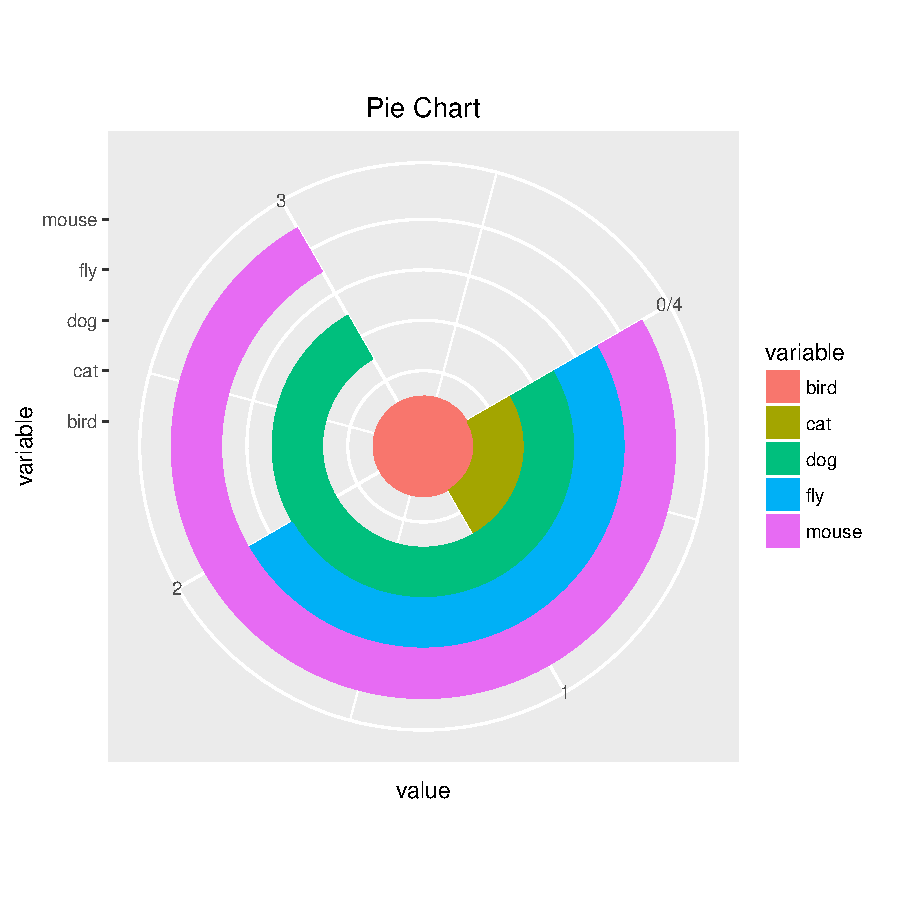
\includegraphics{fig--073}
\label{fig:qplotscatter}
\end{figure}
\end{frame}
%%%%%%%%%%%%%%%%%%%%%%%%%%%%%%%%% slide %%%%%%%%%%%%%%%%%%%%%%%%%%%%%%%%%
\begin{frame}[containsverbatim]  
	\frametitle{ggplot: Arranging Graphics on One Page}
\vspace{0cm}
\tiny 
\begin{Schunk}
\begin{Sinput}
> library(grid)
> a <- ggplot(dsmall, aes(color, price/carat)) + geom_jitter(size=4, alpha = I(1 / 1.5), aes(color=color))
> b <- ggplot(dsmall, aes(color, price/carat, color=color)) + geom_boxplot()
> c <- ggplot(dsmall, aes(color, price/carat, fill=color)) + geom_boxplot() + theme(legend.position = "none")
> grid.newpage() # Open a new page on grid device
> pushViewport(viewport(layout = grid.layout(2, 2))) # Assign to device viewport with 2 by 2 grid layout 
> print(a, vp = viewport(layout.pos.row = 1, layout.pos.col = 1:2))
> print(b, vp = viewport(layout.pos.row = 2, layout.pos.col = 1))
> print(c, vp = viewport(layout.pos.row = 2, layout.pos.col = 2, width=0.3, height=0.3, x=0.8, y=0.8))
\end{Sinput}
\end{Schunk}
\end{frame}
%%%%%%%%%%%%%%%%%%%%%%%%%%%%%%%%% slide %%%%%%%%%%%%%%%%%%%%%%%%%%%%%%%%%
\begin{frame}[containsverbatim]  
	\frametitle{ggplot: Arranging Graphics on One Page}
\vspace{0cm}
\begin{figure}[htbp]
\begin{center}
        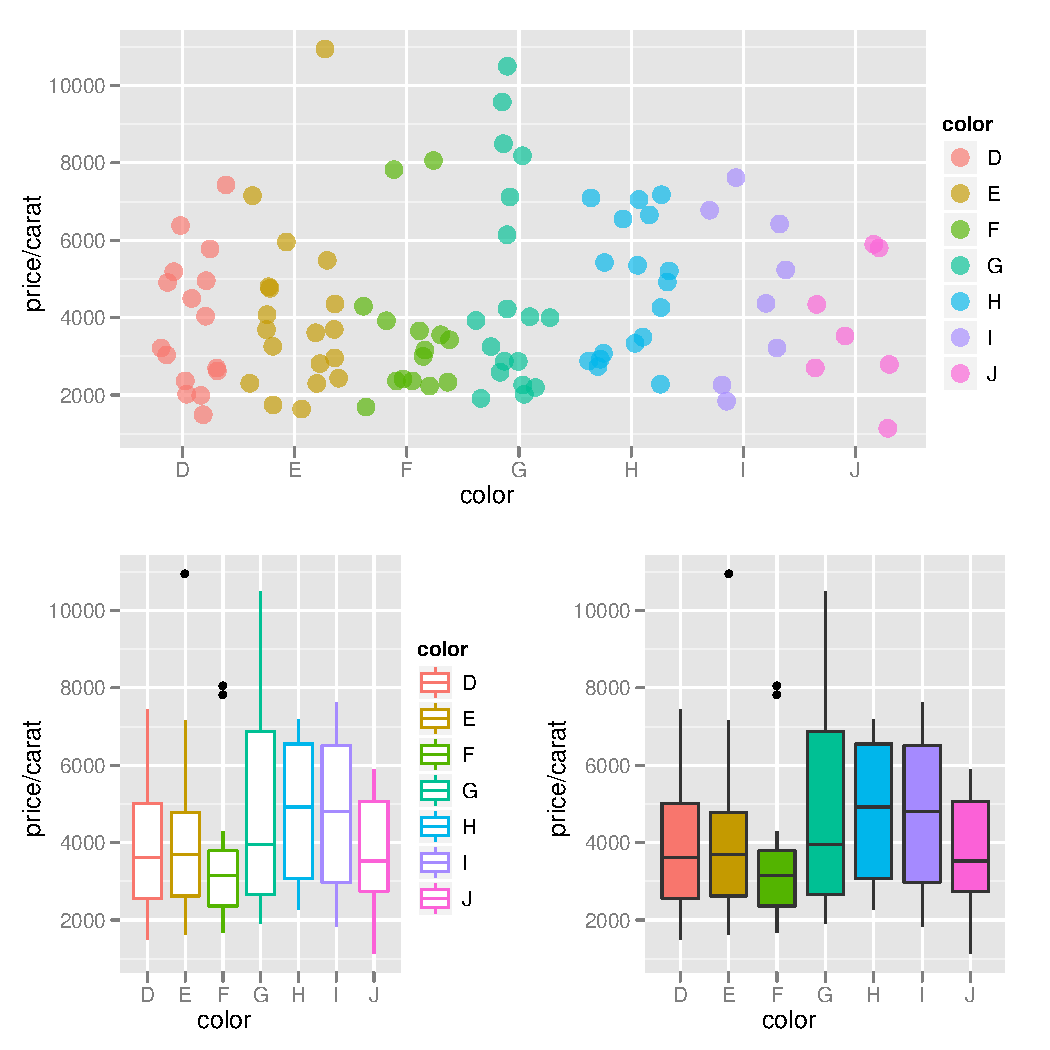
\includegraphics[height=6cm, width=6cm]{arrange.pdf} \\
%\caption{text}
\end{center}
\end{figure}
\end{frame}
%%%%%%%%%%%%%%%%%%%%%%%%%%%%%%%%% slide %%%%%%%%%%%%%%%%%%%%%%%%%%%%%%%%%
\begin{frame}[containsverbatim]  
	\frametitle{ggplot: Inserting Graphics into Plots}
\vspace{0cm}
\tiny
\begin{Schunk}
\begin{Sinput}
> # pdf("insert.pdf")
> print(a)
> print(b, vp=viewport(width=0.3, height=0.3, x=0.8, y=0.8))
> # dev.off()
\end{Sinput}
\end{Schunk}
\begin{figure}[htbp]
\begin{center}
        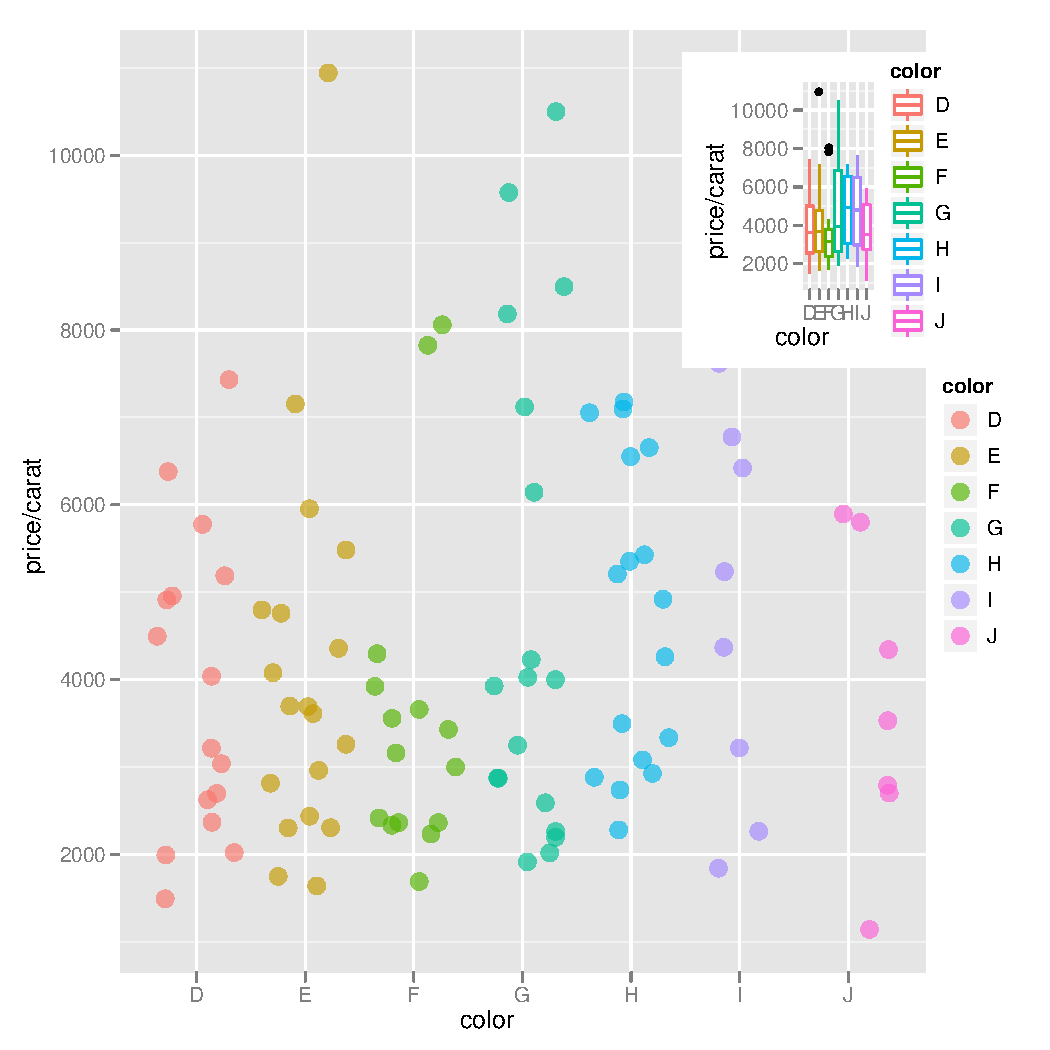
\includegraphics[height=6cm, width=6cm]{insert.pdf} \\
%\caption{text}
\end{center}
\end{figure}
\end{frame}
%%%%%%%%%%%%%%%%%%%%%%%%%%%%%%%%% slide %%%%%%%%%%%%%%%%%%%%%%%%%%%%%%%%%
\section{Specialty Graphics}
%%%%%%%%%%%%%%%%%%%%%%%%%%%%%%%%% SLIDE %%%%%%%%%%%%%%%%%%%%%%%%%%%%%%%%%
\begin{frame}[containsverbatim] % required for xtable!!!!
        \frametitle{Venn Diagrams (Code)}
\tiny
\begin{Schunk}
\begin{Sinput}
> source("http://faculty.ucr.edu/~tgirke/Documents/R_BioCond/My_R_Scripts/overLapper.R")
\end{Sinput}
\end{Schunk}
\begin{Schunk}
\begin{Sinput}
> setlist5 <- list(A=sample(letters, 18), B=sample(letters, 16), C=sample(letters, 20), D=sample(letters, 22), E=sample(letters, 18))
> OLlist5 <- overLapper(setlist=setlist5, sep="_", type="vennsets")
> counts <- sapply(OLlist5$Venn_List, length)
> # pdf("venn.pdf")
> vennPlot(counts=counts, ccol=c(rep(1,30),2), lcex=1.5, ccex=c(rep(1.5,5), rep(0.6,25),1.5))
> # dev.off()
\end{Sinput}
\end{Schunk}
\end{frame}
%%%%%%%%%%%%%%%%%%%%%%%%%%%%%%%%% SLIDE %%%%%%%%%%%%%%%%%%%%%%%%%%%%%%%%%
\begin{frame}[containsverbatim] % required for xtable!!!!
        \frametitle{Venn Diagram (Plot)}
\begin{figure}[htbp]
\begin{center}
        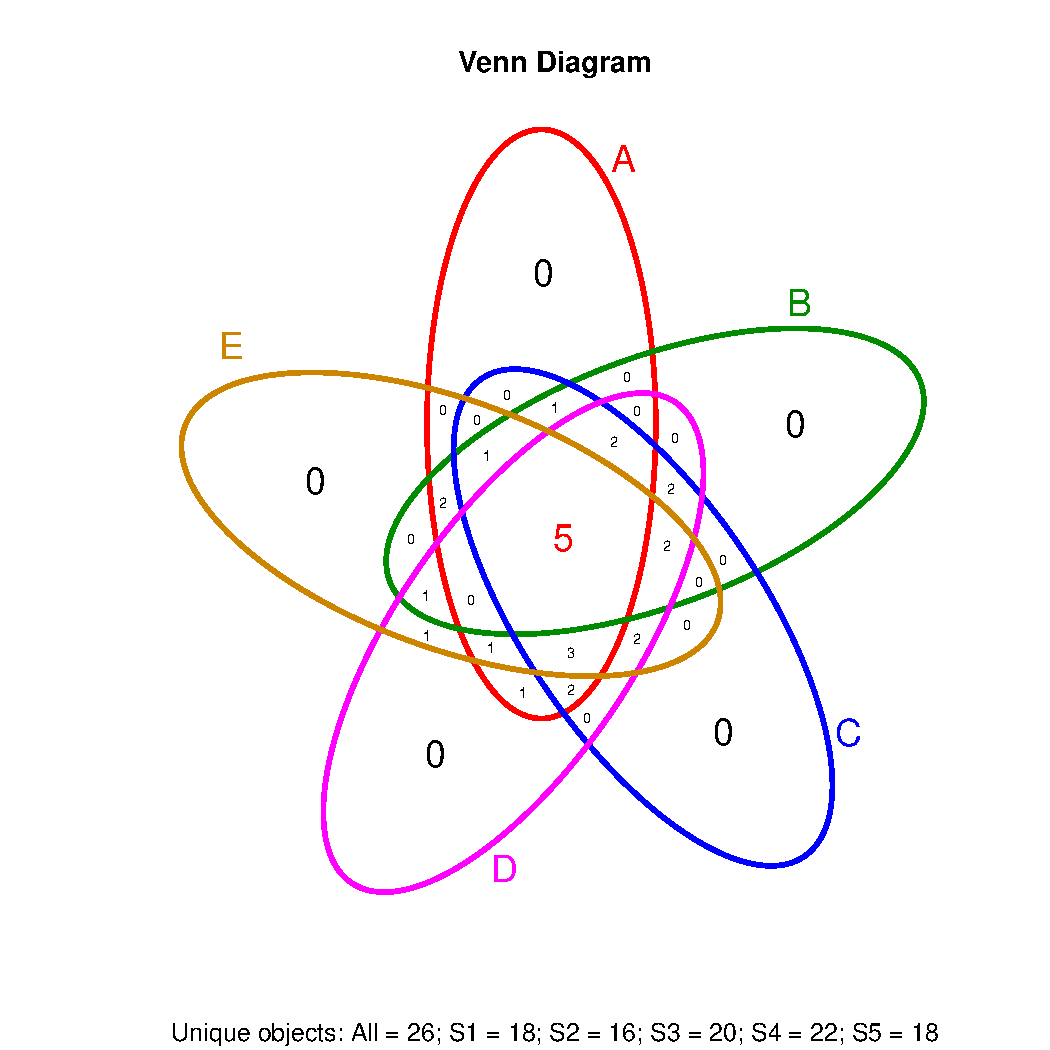
\includegraphics[height=6cm, width=6cm]{venn.pdf} \\
\caption{Venn Diagram}
\end{center}
\end{figure}
\end{frame}
%%%%%%%%%%%%%%%%%%%%%%%%%%%%%%%%% slide %%%%%%%%%%%%%%%%%%%%%%%%%%%%%%%%%
\begin{frame}[containsverbatim]  
	\frametitle{Compound Depictions with ChemmineR}
\tiny 
\begin{figure}
  \centering
\begin{Schunk}
\begin{Sinput}
> library(ChemmineR)
> data(sdfsample)
> plot(sdfsample[1], print=FALSE)
\end{Sinput}
\end{Schunk}
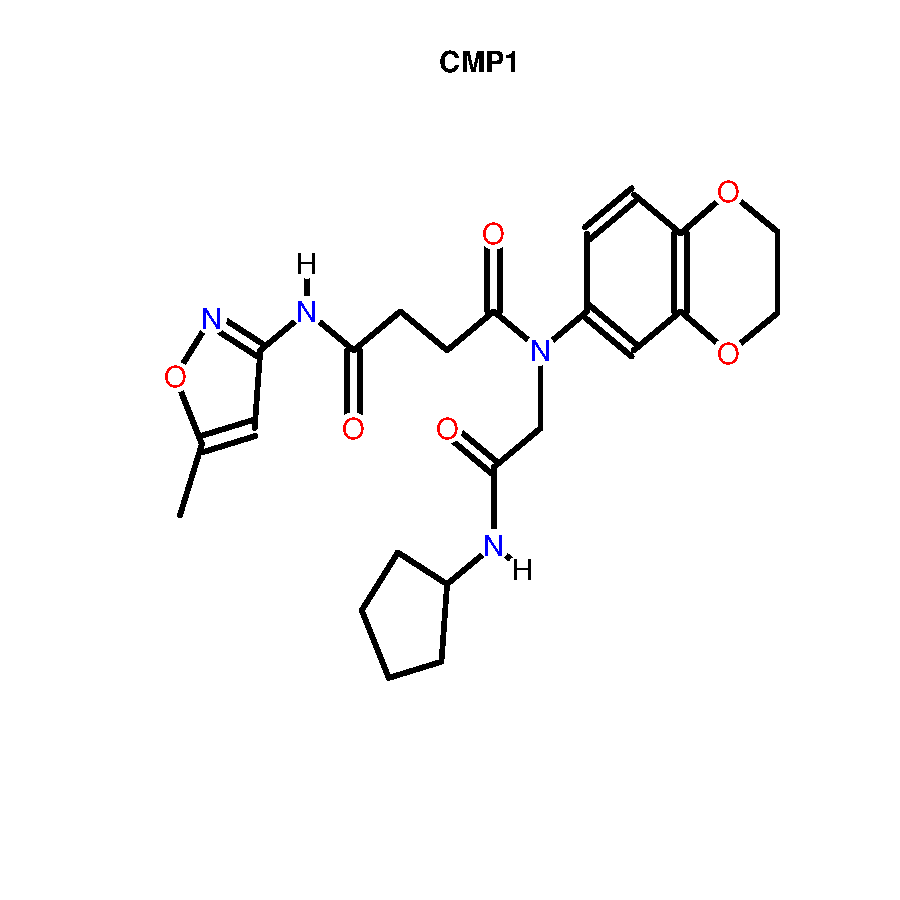
\includegraphics{fig--078}
\label{fig:compounds}
\end{figure}
\end{frame}
%%%%%%%%%%%%%%%%%%%%%%%%%%%%%%%%% slide %%%%%%%%%%%%%%%%%%%%%%%%%%%%%%%%%
\section{Genome Graphics}
%%%%%%%%%%%%%%%%%%%%%%%%%%%%%%%%% slide %%%%%%%%%%%%%%%%%%%%%%%%%%%%%%%%%
\subsection{ggbio}
%%%%%%%%%%%%%%%%%%%%%%%%%%%%%%%%% slide %%%%%%%%%%%%%%%%%%%%%%%%%%%%%%%%%
\begin{frame}[containsverbatim]  
	\frametitle{\Rpackage{ggbio}: A Programmable Genome Browser}
\begin{changemargin}{-0.6cm}{-0.8cm}
\footnotesize 
\begin{itemize}
	\item A genome browser is a visulalization tool for plotting different types of genomic data in separate tracks along chromosomes. 
	\item The \Rpackage{ggbio} package \citep{Yin2012a} facilitates plotting of complex genome data objects, such as read alignments (SAM/BAM), genomic context/annotation information (gff/txdb), variant calls (VCF/BCF), and more. To easily compare these data sets, it extends the faceting facility of \Rpackage{ggplot2} to genome browser-like tracks.
	\item Most of the core object types for handling genomic data with R/Bioconductor are supported: \Robject{GRanges}, \Robject{GAlignments}, \Robject{VCF}, etc. For more details, see Table 1.1 of the \Rpackage{ggbio} vignette \href{http://www.bioconductor.org/packages/release/bioc/vignettes/ggbio/inst/doc/ggbio.pdf}{{\beamerbutton{Link}}}.
	\item \Rpackage{ggbio}'s convenience plotting function is \textcolor{blue}{\Rfunction{autoplot}}. For more customizable plots, one can use the generic \textcolor{blue}{\Rfunction{ggplot}} function.
	\item Apart from the standard \Rfunction{ggplot2} plotting components, \Rfunction{ggbio} defines serval new components useful for genomic data visualization. A detailed list is given in Table 1.2 of the vignette \href{http://www.bioconductor.org/packages/release/bioc/vignettes/ggbio/inst/doc/ggbio.pdf}{{\beamerbutton{Link}}}. 
	\item Useful web sites:
	\begin{itemize}
	\scriptsize
		\item \Rpackage{ggbio} manual \href{http://www.tengfei.name/ggbio/docs/}{{\beamerbutton{Link}}}
		\item \Rpackage{ggbio} functions \href{http://www.tengfei.name/ggbio/docs/man/}{{\beamerbutton{Link}}}
		\item \Rfunction{autoplot} demo \href{http://www.tengfei.name/ggbio/docs/man/autoplot-method.html}{{\beamerbutton{Link}}}
	\end{itemize}
\end{itemize}
\end{changemargin}
\end{frame}
%%%%%%%%%%%%%%%%%%%%%%%%%%%%%%%%% slide %%%%%%%%%%%%%%%%%%%%%%%%%%%%%%%%%
\begin{frame}[containsverbatim]  
	\frametitle{Tracks: Aligning Plots Along Chromosomes}
\tiny 
\begin{figure}
  \centering
\begin{Schunk}
\begin{Sinput}
> library(ggbio)
> df1 <- data.frame(time = 1:100, score = sin((1:100)/20)*10)
> p1 <- qplot(data = df1, x = time, y = score, geom = "line")
> df2 <- data.frame(time = 30:120, score = sin((30:120)/20)*10, value = rnorm(120-30 +1))
> p2 <- ggplot(data = df2, aes(x = time, y = score)) + geom_line() + geom_point(size = 2, aes(color = value))
> tracks(time1 = p1, time2 = p2) + xlim(1, 40) + theme_tracks_sunset()
\end{Sinput}
\end{Schunk}
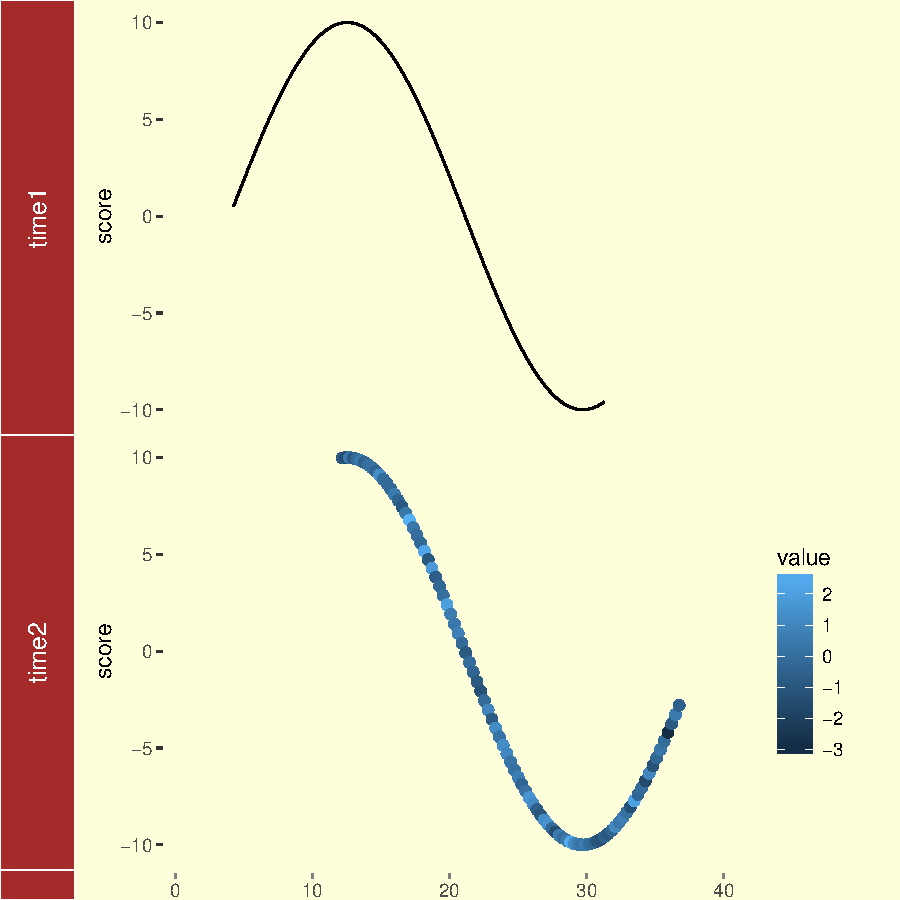
\includegraphics{fig--079}
\label{fig:tracks}
\end{figure}
\end{frame}
%%%%%%%%%%%%%%%%%%%%%%%%%%%%%%%%% slide %%%%%%%%%%%%%%%%%%%%%%%%%%%%%%%%%
\begin{frame}[containsverbatim]  
	\frametitle{Plotting Genomic Ranges}
\scriptsize
\textcolor{blue}{\Robject{GRanges} objects are essential for storing alignment or annotation ranges in R/Bioconductor. The following creates a sample \Robject{GRanges} object and plots its content.}
\tiny 
\begin{figure}
  \centering
\begin{Schunk}
\begin{Sinput}
> library(GenomicRanges)
> set.seed(1); N <- 100; gr <- GRanges(seqnames = sample(c("chr1", "chr2", "chr3"), size = N, replace = TRUE), IRanges(start = sample(1:300, size = N, replace = TRUE), width = sample(70:75, size = N,replace = TRUE)), strand = sample(c("+", "-"), size = N, replace = TRUE), value = rnorm(N, 10, 3), score = rnorm(N, 100, 30), sample = sample(c("Normal", "Tumor"), size = N, replace = TRUE), pair = sample(letters, size = N, replace = TRUE))
> autoplot(gr, aes(color = strand, fill = strand), facets = strand ~ seqnames)
\end{Sinput}
\end{Schunk}
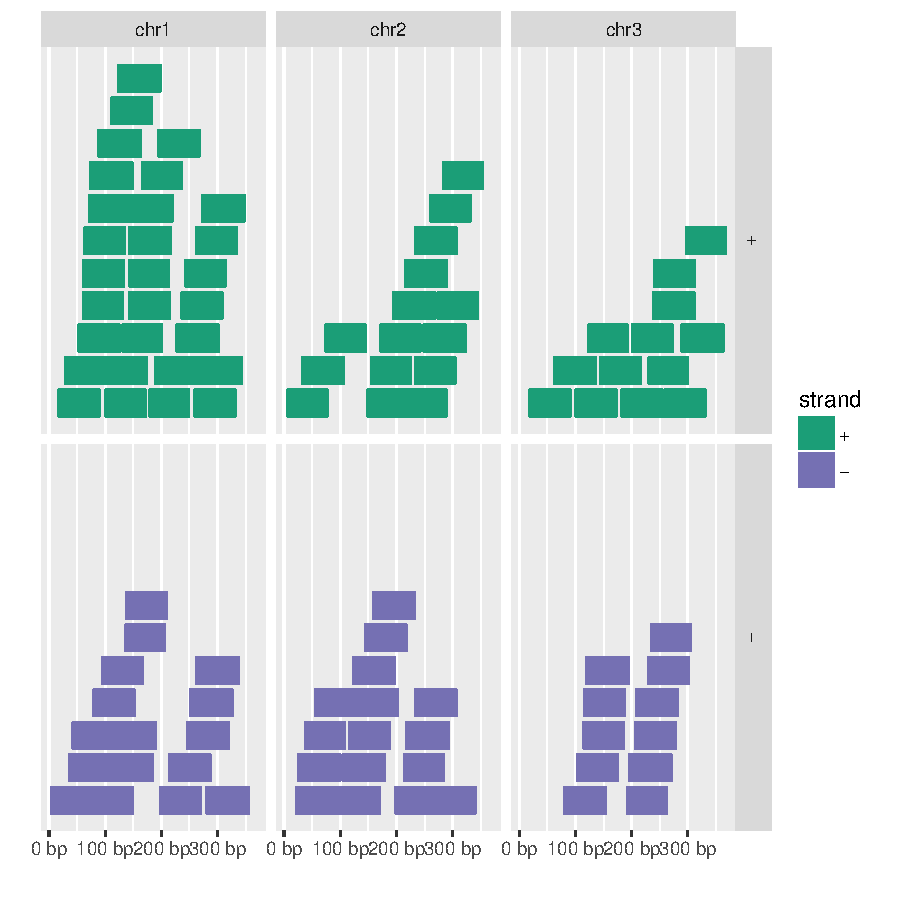
\includegraphics{fig--080}
\label{fig:tracks}
\end{figure}
\end{frame}
%%%%%%%%%%%%%%%%%%%%%%%%%%%%%%%%% slide %%%%%%%%%%%%%%%%%%%%%%%%%%%%%%%%%
\begin{frame}[containsverbatim]  
	\frametitle{Plotting Coverage Instead of Ranges}
\tiny 
\begin{figure}
  \centering
\begin{Schunk}
\begin{Sinput}
> autoplot(gr, aes(color = strand, fill = strand), facets = strand ~ seqnames, stat = "coverage")
\end{Sinput}
\end{Schunk}
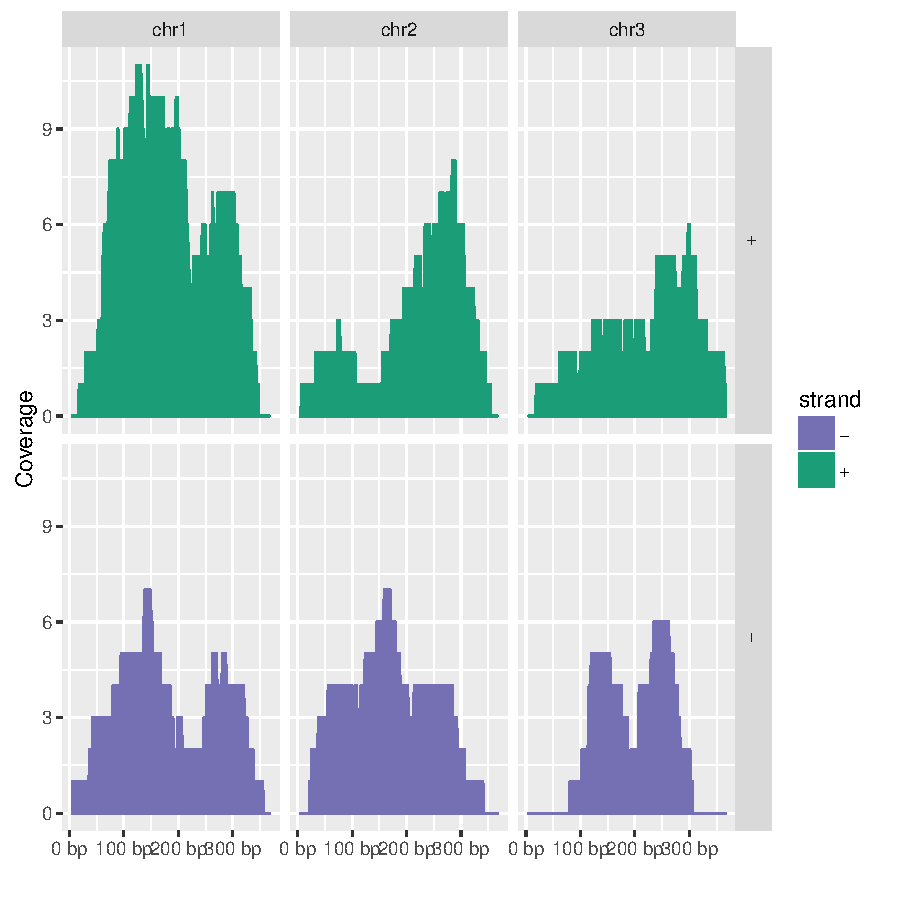
\includegraphics{fig--081}
\label{fig:tracks}
\end{figure}
\end{frame}
%%%%%%%%%%%%%%%%%%%%%%%%%%%%%%%%% slide %%%%%%%%%%%%%%%%%%%%%%%%%%%%%%%%%
\begin{frame}[containsverbatim]  
	\frametitle{Mirrored Coverage Plot}
\tiny 
\begin{figure}
  \centering
\begin{Schunk}
\begin{Sinput}
> pos <- sapply(coverage(gr[strand(gr)=="+"]), as.numeric)
> pos <- data.frame(Chr=rep(names(pos), sapply(pos, length)), Strand=rep("+", length(unlist(pos))), Position=unlist(sapply(pos, function(x) 1:length(x))), Coverage=as.numeric(unlist(pos)))
> neg <- sapply(coverage(gr[strand(gr)=="-"]), as.numeric)
> neg <- data.frame(Chr=rep(names(neg), sapply(neg, length)), Strand=rep("-", length(unlist(neg))), Position=unlist(sapply(neg, function(x) 1:length(x))), Coverage=-as.numeric(unlist(neg)))
> covdf <- rbind(pos, neg)
> p <- ggplot(covdf, aes(Position, Coverage, fill=Strand)) + 
+ 	    geom_bar(stat="identity", position="identity") + facet_wrap(~Chr)
> p
\end{Sinput}
\end{Schunk}
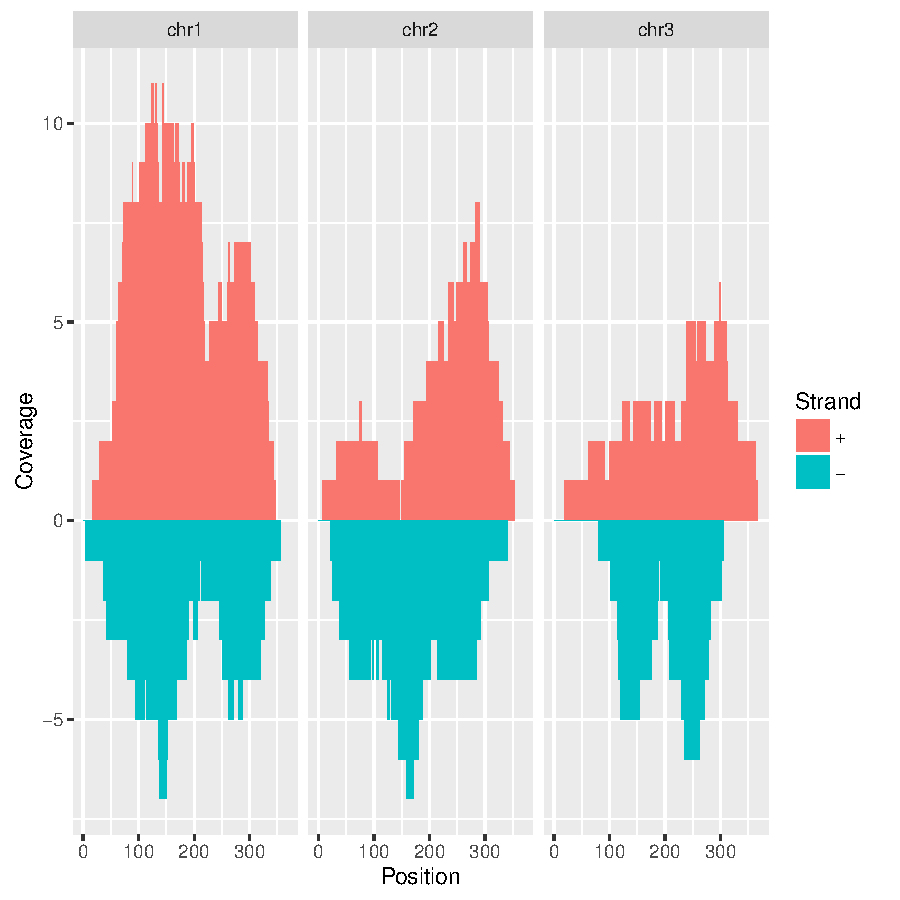
\includegraphics{fig--082}
\label{fig:tracks}
\end{figure}
\end{frame}
%%%%%%%%%%%%%%%%%%%%%%%%%%%%%%%%% slide %%%%%%%%%%%%%%%%%%%%%%%%%%%%%%%%%
\begin{frame}[containsverbatim]  
	\frametitle{Circular Layout}
\tiny 
\begin{figure}
  \centering
\begin{Schunk}
\begin{Sinput}
> ggplot(gr) + layout_circle(aes(fill = seqnames), geom = "rect")
\end{Sinput}
\end{Schunk}
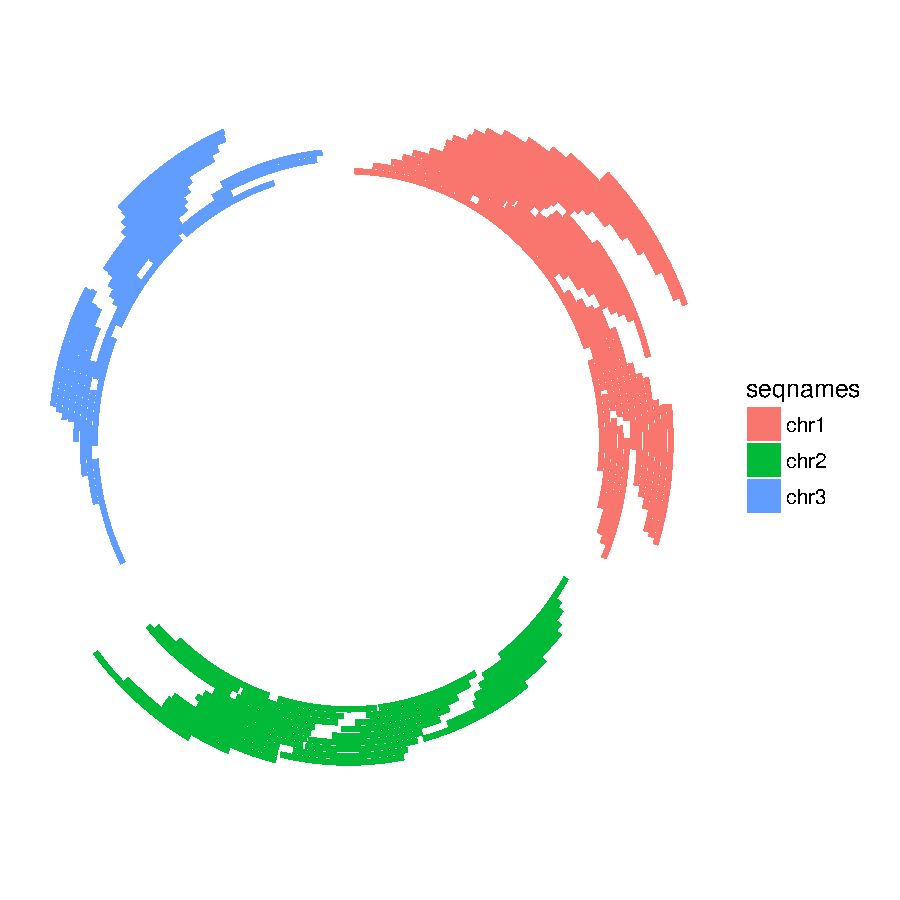
\includegraphics{fig--083}
\label{fig:tracks}
\end{figure}
\end{frame}
%%%%%%%%%%%%%%%%%%%%%%%%%%%%%%%%% slide %%%%%%%%%%%%%%%%%%%%%%%%%%%%%%%%%
\begin{frame}[containsverbatim]  
	\frametitle{More Complex Circular Example}
\tiny 
\begin{Schunk}
\begin{Sinput}
> seqlengths(gr) <- c(400, 500, 700)
> values(gr)$to.gr <- gr[sample(1:length(gr), size = length(gr))]
> idx <- sample(1:length(gr), size = 50)
> gr <- gr[idx]
> ggplot() + layout_circle(gr, geom = "ideo", fill = "gray70", radius = 7, trackWidth = 3) +
+   layout_circle(gr, geom = "bar", radius = 10, trackWidth = 4,
+                 aes(fill = score, y = score)) +
+   layout_circle(gr, geom = "point", color = "red", radius = 14,
+                 trackWidth = 3, grid = TRUE, aes(y = score)) +
+   layout_circle(gr, geom = "link", linked.to = "to.gr", radius = 6, trackWidth = 1)
\end{Sinput}
\end{Schunk}
\end{frame}
%%%%%%%%%%%%%%%%%%%%%%%%%%%%%%%%% slide %%%%%%%%%%%%%%%%%%%%%%%%%%%%%%%%%
\begin{frame}[containsverbatim]  
	\frametitle{Viewing Alignments and Variants}
\vspace{0.3cm}
\scriptsize
\textcolor{blue}{To make the following example work, please download and unpack this data archive \href{http://biocluster.ucr.edu/~tgirke/HTML_Presentations/Manuals/Workshop_Dec_12_16_2013/Rgraphics/data.zip}{{\beamerbutton{Link}}} containing GFF, BAM and VCF sample files.}
\vspace{-0.2cm}
\tiny 
\begin{figure}
  \centering
\begin{Schunk}
\begin{Sinput}
> library(rtracklayer); library(GenomicFeatures); library(Rsamtools); library(GenomicAlignments); library(VariantAnnotation)
> ga <- readGAlignments("./data/SRR064167.fastq.bam", use.names=TRUE, param=ScanBamParam(which=GRanges("Chr5", IRanges(4000, 8000))))
> p1 <- autoplot(ga, geom = "rect")
> p2 <- autoplot(ga, geom = "line", stat = "coverage")
> vcf <- readVcf(file="data/varianttools_gnsap.vcf", genome="ATH1")
> p3 <- autoplot(vcf[seqnames(vcf)=="Chr5"], type = "fixed") + xlim(4000, 8000) + theme(legend.position = "none", axis.text.y = element_blank(), axis.ticks.y=element_blank())
> txdb <- makeTxDbFromGFF(file="./data/TAIR10_GFF3_trunc.gff", format="gff3")
> p4 <- autoplot(txdb, which=GRanges("Chr5", IRanges(4000, 8000)), names.expr = "gene_id")
> tracks(Reads=p1, Coverage=p2, Variant=p3, Transcripts=p4, heights = c(0.3, 0.2, 0.1, 0.35)) + ylab("")
\end{Sinput}
\end{Schunk}
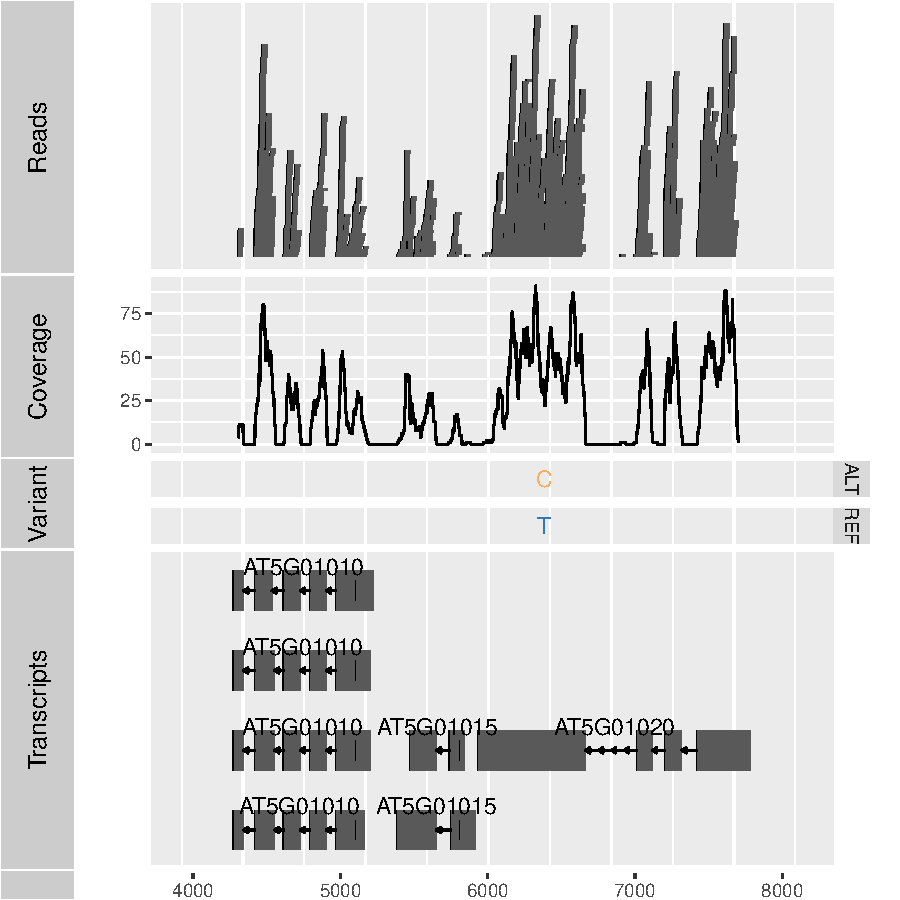
\includegraphics{fig--085}
\label{fig:tracks}
\end{figure}
\end{frame}
%%%%%%%%%%%%%%%%%%%%%%%%%%%%%%%%% slide %%%%%%%%%%%%%%%%%%%%%%%%%%%%%%%%%
\begin{frame}[containsverbatim]  
	\frametitle{Additional Sample Plots}
\begin{itemize}
	\item \Rfunction{autoplot} demo \href{http://www.tengfei.name/ggbio/docs/man/autoplot-method.html}{{\beamerbutton{Link}}}
\end{itemize}
\end{frame}
%%%%%%%%%%%%%%%%%%%%%%%%%%%%%%%%% slide %%%%%%%%%%%%%%%%%%%%%%%%%%%%%%%%%
\subsection{Additional Genome Graphics}
%%%%%%%%%%%%%%%%%%%%%%%%%%%%%%%%% slide %%%%%%%%%%%%%%%%%%%%%%%%%%%%%%%%%
\begin{frame}[containsverbatim]  
	\frametitle{Additional Packages for Visualizing Genome Data}
\footnotesize 
\begin{itemize}
	\item Gviz \href{http://www.bioconductor.org/packages/devel/bioc/html/Gviz.html}{{\beamerbutton{Link}}}
	\item RCircos \citep{Zhang2013a} \href{http://cran.us.r-project.org/web/packages/RCircos/index.html}{{\beamerbutton{Link}}}
	\item Genome Graphs \href{http://bioconductor.org/packages/release/bioc/html/GenomeGraphs.html}{{\beamerbutton{Link}}}
	\item genoPlotR \href{http://genoplotr.r-forge.r-project.org/}{{\beamerbutton{Link}}}
\end{itemize}
\end{frame}
%%%%%%%%%%%%%%%%%%%%%%%%%%%%%%%%% SLIDE %%%%%%%%%%%%%%%%%%%%%%%%%%%%%%%%%
\section{Genome Browser: IGV}
%%%%%%%%%%%%%%%%%%%%%%%%%%%%%%%%% SLIDE %%%%%%%%%%%%%%%%%%%%%%%%%%%%%%%%%
\begin{frame}[containsverbatim]  
	\frametitle{Alignment Viewing in IGV}
\vspace{1cm}
\begin{changemargin}{-0.5cm}{-0.5cm}
\tiny
\textcolor{blue}{View results in IGV}
\begin{itemize}
\item Download and open IGV\href{http://www.broadinstitute.org/igv/download}{{\beamerbutton{Link}}}
\item Select in menu in top left corner \texttt{A. thaliana (TAIR10)}
\item Upload the following indexed/sorted Bam files with \texttt{File -> Load from URL...}
\end{itemize}
\begin{Schunk}
\begin{Sinput}
http://faculty.ucr.edu/~tgirke/HTML_Presentations/Manuals/Workshop_Dec_6_10_2012/Rrnaseq/results/SRR064154.fastq.bam
http://faculty.ucr.edu/~tgirke/HTML_Presentations/Manuals/Workshop_Dec_6_10_2012/Rrnaseq/results/SRR064155.fastq.bam
http://faculty.ucr.edu/~tgirke/HTML_Presentations/Manuals/Workshop_Dec_6_10_2012/Rrnaseq/results/SRR064166.fastq.bam
http://faculty.ucr.edu/~tgirke/HTML_Presentations/Manuals/Workshop_Dec_6_10_2012/Rrnaseq/results/SRR064167.fastq.bam
\end{Sinput}
\end{Schunk}
\begin{itemize}
\item To view area of interest, enter its coordinates \texttt{Chr1:49,457-51,457} in position menu on top.
\end{itemize}
\begin{figure}

        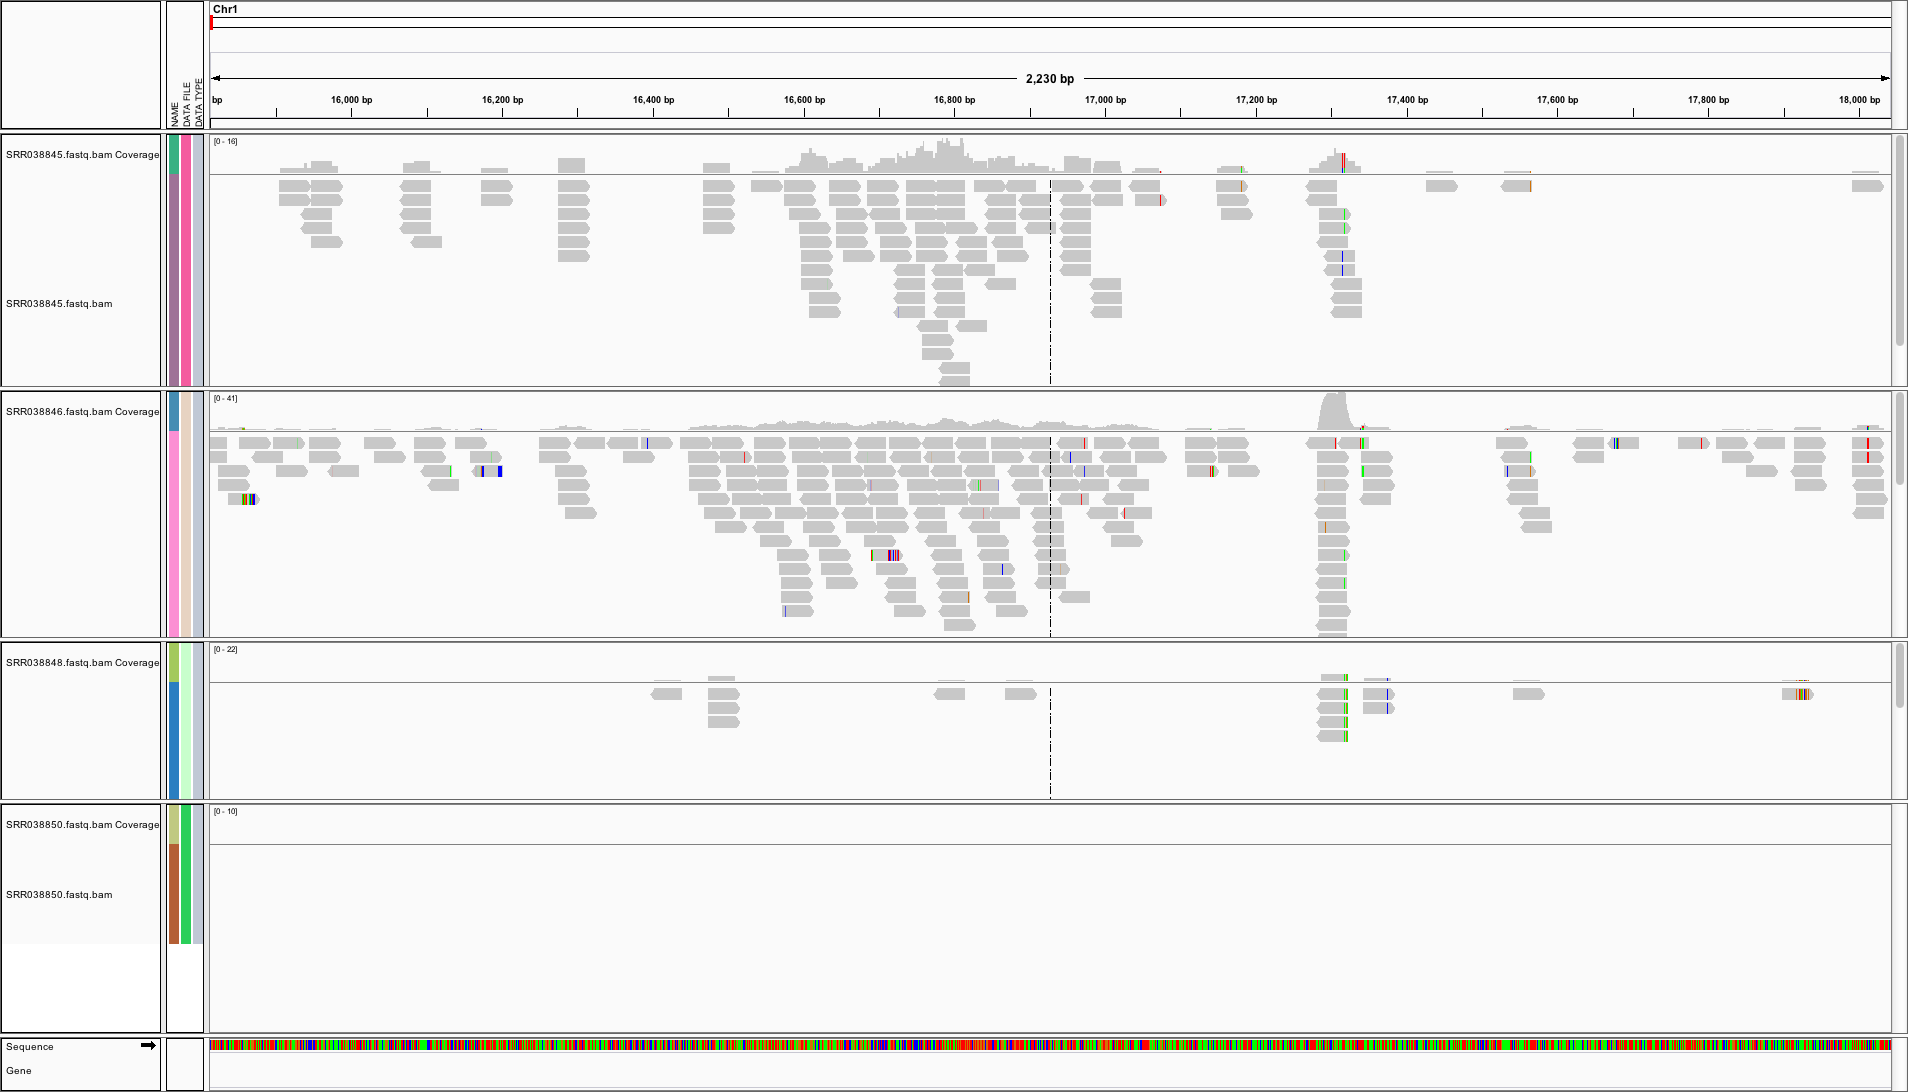
\includegraphics[width=65mm] {./images/igv_peak_3.png} \\
\end{figure}
\end{changemargin}
\end{frame}
%%%%%%%%%%%%%%%%%%%%%%%%%%%%%%%%% SLIDE %%%%%%%%%%%%%%%%%%%%%%%%%%%%%%%%%
\begin{frame}
	\frametitle{Create symbolic links for viewing BAM files in IGV}
\begin{itemize}
	\item systemPipeR: utilities for building NGS analysis pipelines \href{https://github.com/tgirke/systemPipeR}{{\beamerbutton{Link}}} \\
	\vspace{0.3cm}
	\scriptsize
	\hspace{0.5cm} \textcolor{blue}{\texttt{library("systemPipeR")}} \\
	\hspace{0.5cm} \textcolor{blue}{\texttt{symLink2bam(sysargs=args, htmldir=c("~/.html/", "somedir/"), }} \\ 
	\hspace{1.5cm} \textcolor{blue}{\texttt{urlbase="http://myserver.edu/~username/", }} \\
	\hspace{1.5cm} \textcolor{blue}{\texttt{urlfile="IGVurl.txt")}}
\end{itemize}
\end{frame}
%%%%%%%%%%%%%%%%%%%%%%%%%%%% REFERENCE LIST %%%%%%%%%%%%%%%%%%%%%%%%%%%%%
\def\newblock{\hskip .11em plus .33em minus .07em} % Important line to support typical BibTex behavior in Beamer slide presentation
\begin{frame}[allowframebreaks]{Bibliography}
\scriptsize
\bibliographystyle{/Users/tgirke/GoogleDrive/Manuscripts/BibTeX/elsart-harv.bst} % Uses style file "elsart-harv.bst" (Plant Physiology) AND requires in preamble \usepackage{natbib}; many more styles can be found at http://jo.irisson.free.fr/bstdatabase/
\bibliography{/Users/tgirke/GoogleDrive/Manuscripts/BibTeX/MyBibTex.bib} % Expects bibliography file "MyBibTex.bib"
% \nocite{Mistry2007a, Smola2003a, vanderWalt2006a, Ruan2008a, Ivanciuc2007a, Pugalenthi2008a, Wu2009a, Sankararaman2008a, Alterovitz2009a, Salzberg2008a} % includes selected references without citing them
% \nocite{*} % includes all references from a bibtex database
\end{frame}
%%%%%%%%%%%%%%%%%%%%%%%%%%%% REFERENCE LIST %%%%%%%%%%%%%%%%%%%%%%%%%%%%%
\end{document}


